%Version 3.1 December 2024
% See section 11 of the User Manual for version history
%
%%%%%%%%%%%%%%%%%%%%%%%%%%%%%%%%%%%%%%%%%%%%%%%%%%%%%%%%%%%%%%%%%%%%%%
%%                                                                 %%
%% Please do not use \input{...} to include other tex files.       %%
%% Submit your LaTeX manuscript as one .tex document.              %%
%%                                                                 %%
%% All additional figures and files should be attached             %%
%% separately and not embedded in the \TeX\ document itself.       %%
%%                                                                 %%
%%%%%%%%%%%%%%%%%%%%%%%%%%%%%%%%%%%%%%%%%%%%%%%%%%%%%%%%%%%%%%%%%%%%%

%%\documentclass[referee,sn-basic]{sn-jnl}% referee option is meant for double line spacing

%%=======================================================%%
%% to print line numbers in the margin use lineno option %%
%%=======================================================%%

%%\documentclass[lineno,pdflatex,sn-basic]{sn-jnl}% Basic Springer Nature Reference Style/Chemistry Reference Style

%%=========================================================================================%%
%% the documentclass is set to pdflatex as default. You can delete it if not appropriate.  %%
%%=========================================================================================%%

%%\documentclass[sn-basic]{sn-jnl}% Basic Springer Nature Reference Style/Chemistry Reference Style

%%Note: the following reference styles support Namedate and Numbered referencing. By default the style follows the most common style. To switch between the options you can add or remove “Numbered” in the optional parenthesis. 
%%The option is available for: sn-basic.bst, sn-chicago.bst%  
 
%%\documentclass[pdflatex,sn-nature]{sn-jnl}% Style for submissions to Nature Portfolio journals
%%\documentclass[pdflatex,sn-basic]{sn-jnl}% Basic Springer Nature Reference Style/Chemistry Reference Style
%%\documentclass[pdflatex,sn-mathphys-num]{sn-jnl}% Math and Physical Sciences Numbered Reference Style
%%\documentclass[pdflatex,sn-mathphys-ay]{sn-jnl}% Math and Physical Sciences Author Year Reference Style
%%\documentclass[pdflatex,sn-aps]{sn-jnl}% American Physical Society (APS) Reference Style
%%\documentclass[pdflatex,sn-vancouver-num]{sn-jnl}% Vancouver Numbered Reference Style
\documentclass[pdflatex,sn-vancouver-ay]{sn-jnl}% Vancouver Author Year Reference Style
%%\documentclass[pdflatex,sn-apa]{sn-jnl}% APA Reference Style
%%\documentclass[pdflatex,sn-chicago]{sn-jnl}% Chicago-based Humanities Reference Style

%%%% Standard Packages
%%<additional latex packages if required can be included here>

\usepackage{graphicx}%
\usepackage{multirow}%
\usepackage{amsmath,amssymb,amsfonts}%
\usepackage{amsthm}%
\usepackage{mathrsfs}%
\usepackage[title]{appendix}%
\usepackage{xcolor}%
\usepackage{textcomp}%
\usepackage{manyfoot}%
\usepackage{booktabs}%
\usepackage{algorithm}%
\usepackage{algorithmicx}%
\usepackage{algpseudocode}%
\usepackage{listings}%
%%%%

%%%%%=============================================================================%%%%
%%%%  Remarks: This template is provided to aid authors with the preparation
%%%%  of original research articles intended for submission to journals published 
%%%%  by Springer Nature. The guidance has been prepared in partnership with 
%%%%  production teams to conform to Springer Nature technical requirements. 
%%%%  Editorial and presentation requirements differ among journal portfolios and 
%%%%  research disciplines. You may find sections in this template are irrelevant 
%%%%  to your work and are empowered to omit any such section if allowed by the 
%%%%  journal you intend to submit to. The submission guidelines and policies 
%%%%  of the journal take precedence. A detailed User Manual is available in the 
%%%%  template package for technical guidance.
%%%%%=============================================================================%%%%

%% as per the requirement new theorem styles can be included as shown below
\theoremstyle{thmstyleone}%
\newtheorem{theorem}{Theorem}%  meant for continuous numbers
%%\newtheorem{theorem}{Theorem}[section]% meant for sectionwise numbers
%% optional argument [theorem] produces theorem numbering sequence instead of independent numbers for Proposition
\newtheorem{proposition}[theorem]{Proposition}% 
%%\newtheorem{proposition}{Proposition}% to get separate numbers for theorem and proposition etc.

\theoremstyle{thmstyletwo}%
\newtheorem{example}{Example}%
\newtheorem{remark}{Remark}%

\theoremstyle{thmstylethree}%
\newtheorem{definition}{Definition}%

\raggedbottom
%%\unnumbered% uncomment this for unnumbered level heads

% New commands
\newcommand{\Rlang}{\texttt{R}}
\newcommand{\julia}{\texttt{Julia}}
\newcommand{\RTTE}{\texttt{TrialEmulation}}
\newcommand{\juliaTTE}{\texttt{TargetTrialEmulation.jl}}



\begin{document}

\title[Article Title]{Improving Causal Inference from Observational Data: A Comparative Analysis of Confidence Interval Methods in Sequential Target Trial Emulation}

%%=============================================================%%
%% GivenName	-> \fnm{Joergen W.}
%% Particle	-> \spfx{van der} -> surname prefix
%% FamilyName	-> \sur{Ploeg}
%% Suffix	-> \sfx{IV}
%% \author*[1,2]{\fnm{Joergen W.} \spfx{van der} \sur{Ploeg} 
%%  \sfx{IV}}\email{iauthor@gmail.com}
%%=============================================================%%

\author[1]{\fnm{Florian} \sur{Metwaly}}

\author{\fnm{Oisín} \sur{Ryan}}
\equalcont{Supervisors}

\author{\fnm{Wouter} \sur{van Amsterdam}}
\equalcont{Supervisors}

\affil[]{Student Number: 778265}

\affil[]{12th May 2025}


%%==================================%%
%% Sample for unstructured abstract %%
%%==================================%%

% \abstract{The abstract serves both as a general introduction to the topic and as a brief, non-technical summary of the main results and their implications. Authors are advised to check the author instructions for the journal they are submitting to for word limits and if structural elements like subheadings, citations, or equations are permitted.}

%%================================%%
%% Sample for structured abstract %%
%%================================%%

\abstract{
\textbf{Background:} 
 Sequential Target Trial Emulation (TTE) is a framework that is gaining popularity to estimate causal effects from observational data when a randomized control trial (RCT) is not feasible. As sequential TTE involves copying data from the observational dataset multiple times, the assumption of independence between observations is violated, and confidence intervals (CI) can no longer be estimated by standard estimation approaches. While sandwich-type estimators are commonly implemented in statistical software for CI estimation, the non-parametric bootstrap is the recommended method for CI estimation in the TTE literature. We compare the performance of the two approaches and present the \julia{} package \juliaTTE{}, for computationally efficient estimation of bootstrap CIs in the context of sequential TTE.
 
\textbf{Methods:} 
 In a simulation study, we compare the performance of the sandwich-type against two types of non-parametric bootstrap CI estimation: the percentile and the empirical bootstrap. We test the estimators across 81 scenarios, varying the sample sizes, confounding strength, outcome prevalence, and treatment prevalence. We compare their performance regarding their coverage, width, bias-eliminated coverage, and power.
 
\textbf{Results:} 
 Our simulation study finds that both bootstrap methods, percentile and empirical, more frequently achieved coverage closer to the nominal 95\% level, particularly in small sample sizes, and produced narrower confidence intervals than the sandwich estimator. Although the sandwich-type estimator found consistently higher statistical power, this finding is most likely attributable to the sandwich-type estimator being biased upwards. Bias-eliminated coverage analysis suggested that coverage differences were primarily driven by bias in the point estimates, particularly at low event rates and later follow-up times.
 
\textbf{Conclusion:} 
 While this study confirms bootstrap’s potential, limitations of the percentile and empirical approaches, such as sensitivity to skewed distributions and a biased estimator, suggest the need for more robust methods. Advanced techniques like the bias-corrected and accelerated (BCa) bootstrap may provide improved inference in complex TTE settings. Future work should focus on benchmarking these methods using the evaluation framework employed in this study, coverage, width, and bias-eliminated coverage. It should additionally incorporate assessments of power and type I error control, and further focus on computational efficiency. 
}

\keywords{Sequential Target Trial Emulation, Bootstrap, Sandwich Estimator, Observational Data, Causal Inference}

%%\pacs[JEL Classification]{D8, H51}

%%\pacs[MSC Classification]{35A01, 65L10, 65L12, 65L20, 65L70}

\maketitle

\section{Introduction}\label{Intro}
Randomised Control Trials (RCT) are the gold standard of causal inference. However, due to practical and ethical constraints, conducting an RCT is not always feasible \citep{hernanUsingBigData2016, sanson-fisherLimitationsRandomizedControlled2007}. Gaining causal insights from observational data has been a long prevailing topic of research \citep{woldCausalInferenceObservational1956, nicholsCausalInferenceObservational}. In health sciences, large-scale observational datasets such as electronic health record databases are increasingly used for causal analyses when RCTs are not feasible \citep{bakkerAnalysingElectronicHealth2021}. 

When randomization is not possible or available, confounding bias must be addressed, for example, by measuring and statistically adjusting for confounding variables. Common methods are using matching or weighting methods for observed confounding \citep{schaferAverageCausalEffects2008} or adjusting the design for unobserved confounding \citep{igelstromCausalInferenceEffect2022, listlCausalInferenceObservational2016}.

Increasingly, researchers in the health sciences have recognized that while mimicking randomization and adjusting for confounding are necessary steps, they are not sufficient to draw valid causal inferences from observational data. The reason for this is that, when analyzing observational data, the researcher is free to make design choices that may accidentally introduce different forms of selection biases or lead to a mismatch between the target quantity being estimated and the quantity of clinical interest \citep{fuTargetTrialEmulation2023}. 

Immortal time bias, a type of bias that occurs when a period of time during which the event of interest cannot occur is incorrectly classified in the analysis, is a specific form of selection bias often seen in observational studies \citep{yadavImmortalTimeBias2021, hernanStructuralDescriptionBiases2025}. For example, in a vaccination study, individuals are enrolled in the study and they are eligible for vaccination from this time point on. However, the vaccine administration often occurs a few days after enrollment. Suppose this period between enrollment and vaccination is misclassified as time during which the individual is unvaccinated and not accounted for in the analysis. In that case, it results in an artificially lower infection rate for the vaccinated group. This is because during this interval, the patient cannot get infected with COVID-19, effectively rendering them ``immortal" with respect to the outcome. Such misclassification is typically referred to as immortal time bias \citep{hernanStructuralDescriptionBiases2025}.


\subsection{Target Trial Emulation}
Target Trial Emulation (TTE) is a methodological framework for designing observational data analyses to enable valid causal inference. TTE has specifically been developed to prevent the introduction of biases through research design. To perform TTE, one must first specify the ideal randomized control trial, the so-called target trial, which one would perform if feasible. The design of the TTE then mimics this idealized RCT as closely as possible \citep{hernanObservationalStudiesAnalyzed2008, hernanTargetTrialFramework2025}. For this, a detailed trial protocol is typically specified \citep{hernanObservationalStudiesAnalyzed2008, hernanTargetTrialFramework2025}. 

A key concept of TTE is that of $t_0$ alignment. The $t_0$ describes the moment at which eligibility is determined, treatment is assigned and started, and the follow-up period starts \citep{hernanObservationalStudiesAnalyzed2008, hernanTargetTrialFramework2025}. Extending the COVID-19 vaccine example, EHR data could be used to study the effectiveness of the COVID-19 vaccine. Suppose a dataset that includes patient data from January 1st, 2020, to December 31st, 2022, including their vaccination status, an indicator of whether they are eligible to be vaccinated, possible confounders, and an indicator of whether COVID-19 occurred or not. To emulate the target trial, the data can be analyzed by choosing an enrollment date, for example, January 1st, 2020. Every eligible individual on January 1st, 2020, gets ``enrolled" in the trial, and their follow-up time starts. Individuals vaccinated on this date now form the treatment group; unvaccinated individuals form the control group. After the previously defined end date, say December 31st, 2022, the resulting subset can be used to estimate causal effects from this dataset. Notably, the model still has to adjust for confounding, for example, by using inverse propensity score weighting, which is not discussed further at this point.

To align $t_0$, a critical design choice must be made \citep{fuStartingRightAligning2025}. In the COVID-19 vaccine example, a single $t_0$ is selected as the starting point of the follow-up time. However, this potentially leads to losing a large number of observations, due to them not being eligible at the chosen $t_0$, and can result in very few observations in the treatment arm, as individuals who receive the vaccination at a later time point are excluded from the analysis. Alternatively, the researcher can select \emph{all} time points. When opting for this option, we speak of sequential Target Trial Emulation.


\subsection{Sequential Target Trial Emulation}
The core idea behind sequential Target Trial Emulation is that the specific date at which the trial starts is not of primary interest. Therefore, it is possible to iterate through all observed time points and start a new trial with all eligible individuals and their follow-up observations at each time point. Returning to the vaccination example, the eligible individuals on January 1st will now define the first trial. The same process will now be repeated for January 2nd. All individuals who are eligible on January 2nd and their follow-up times are selected and enrolled in the second trial. This process is repeated for all observation points, forming a large dataset containing all emulated trials, with any individual possibly being part of multiple trials. By reassigning $t_0$ at every eligible time point, each separate trial includes only the correctly aligned follow-up period, excluding any interval during which the outcome, like the COVID-19 infection, could not occur due to the individuals being in an ``immortal" phase. This prevents the introduction of immortal time bias \citep{hernanStructuralDescriptionBiases2025, hernanTargetTrialFramework2025}. To clearly illustrate the construction of the sequentially emulated dataset, pseudocode is provided in Appendix~\ref{sec:apxseqtte}.

\subsection{Variance Estimation}\label{VarEst}

Two problems arise for the variance estimation in a sequential TTE setting. The first issue arises from sequential TTE generating multiple trials over time by repeatedly applying the trial eligibility criteria at each time point. In practice, any individual may be subject to numerous trials, which violates the standard assumption of independence between observations, as any individual potentially contributes data to multiple emulated trials \citep{hernanUsingBigData2016}. This dependency is an inherent consequence of the sequential TTE framework.

Second, as mentioned earlier, a common method to account for confounding bias is using inverse probability of treatment weighting (IPTW). Additionally, time-to-event data typically contains censored observations. Those are also accounted for when performing an analysis using the sequential TTE framework through inverse probability of censor weighting (IPCW) \citep{hernanObservationalStudiesAnalyzed2008}. Censoring itself is not further discussed in this work, as the specific form of weighting is not central to the methodological evaluation; rather, the focus lies on the general impact of using inverse probability weights (IPW). As IPWs are often unstable, they introduce variability into the estimates, especially when the probabilities of treatment or censoring are close to $0$ or $1$. This variability can lead to underestimated standard errors, resulting in overly narrow confidence intervals and overconfident conclusions if not appropriately addressed \citep{austinMovingBestPractice2015, austinVarianceEstimationWhen2016}. While this problem is not inherent to the sequential TTE design, inverse probability weighting is the recommended, and in practice most often applied approach, to adjust for confounding and censoring \citep{hernanTargetTrialFramework2025, hernanObservationalStudiesAnalyzed2008}.

A common solution to these issues is using sandwich-type variance estimators, as proposed by \cite{linRobustInferenceCox1989}, which provide robust standard error estimates that remain valid under such complexities, and are commonly used to construct confidence intervals (CI). Due to its common integration in statistical software \citep{hernanCausalInferenceWhat}, it is a frequently used method in the literature (see, e.g. \cite{wuOutcomesReinitiatingDirect2025, liADHDPharmacotherapyMortality2024, scolaImplementationTrialEmulation2023}). 

Although the sandwich-type variance estimator is commonly used in practice, the TTE literature typically recommends using a non-parametric bootstrap approach to estimate the variance and confidence intervals \citep{maringeReflectionModernMethods2020, hernanUsingBigData2016, bakkerAnalysingElectronicHealth2021}. This is due to previous findings, for example in the survival analysis literature, where bootstrapping CIs in comparison with unadjusted approaches or sandwich-type estimators, were found to produce approximately correct standard errors and correct coverage rates for CIs, outperforming the unadjusted model and sandwich-type estimators \citep{austinVarianceEstimationWhen2016}.

The non-parametric bootstrap is a powerful tool for inference in cases of violation of various assumptions. Bootstrapping is a resampling technique that involves repeatedly sampling with replacement from the observed data to generate new datasets, which are then used to estimate the sampling distribution of a statistic. Due to the repeated resampling, bootstrap confidence intervals can be computationally intensive, posing practical challenges in large-scale settings such as EHR data. While computational optimizations for the bootstrap exist at the cost of additional assumptions, we do not consider them further here (see, e.g. \cite{liGeneralizedBootstrapProcedure2024, binderDesignBasedMethodsSurvey}).

In this paper, we systematically evaluate the properties of non-parametric bootstrap confidence intervals within the sequential TTE framework, comparing them to widely used sandwich-type estimators under realistic simulation settings. In Section~\ref{sec:Methods} we describe the model on which the sequential TTE framework is applied and how confidence intervals can be estimated. Further in Section~\ref{sec:juliaTTE} we present a software implementation of bootstrapped confidence intervals. Section~\ref{sec:SimulationStudy} describes the simulation study which we use to evaluate the performance of the non-parametric bootstrap compared to sandwich-type estimators. The simulation study results are presented in Section~\ref{sec:Results} and discussed in Section~\ref{sec:Discussion}.

\section{Methods}\label{sec:Methods}

In the following section, we describe the methodological framework used to evaluate the performance of the non-parametric bootstrap in comparison to sandwich-type estimators for estimating confidence intervals in a sequential TTE setting. Further, we introduce the \juliaTTE{} package, a practical implementation of sequential TTE in the \julia{} programming language. Finally, we describe the simulation study designed to assess and compare the performance of both variance estimation approaches across a range of data-generating scenarios.

\subsection{Defining the Estimand}\label{DefineEst}

Two types of analysis are common in clinical research: the intention-to-treat (ITT) and per-protocol (PP) analyses. In a PP analysis, individuals are analyzed according to the treatment they actually received, excluding those who deviated from the study protocol. In an ITT analysis, the individuals are analyzed according to their initially assigned treatment, regardless of subsequent treatment changes  \citep{tripepiIntentionTreatProtocol2020}.
As the validity of bootstrap confidence intervals has already been investigated in a PP analysis \citep{limozinInferenceProceduresSequential2024}, the following study will compare the sandwich-type estimator and bootstrap confidence intervals in the context of an ITT analysis.

We assume a setting in which a single individual is observed regularly over a set period of time $K$. The start of follow-up time is denoted by $k = 0$. Information about treatment status $A_k$, eligibility $E_k$, time-varying confounders $L_k$, and the binary outcome of interest $Y_k$ is collected at each timepoint $k = 0, 1, 2, \dots, K$. Time-invariant confounders are denoted by $V$, and time-varying confounders are fixed to their baseline values and denoted by $L_0$, due to performing an ITT analysis. Treatment status $A_k$ is binary, taking values $a \in \{0, 1\}$, representing treated and untreated, respectively. Once an individual experiences the event ($Y_k = 1$), they are no longer followed and are excluded from the dataset in subsequent time points.

The cumulative survival distribution under treatment strategy $a$, denoted by $S_a(k)$, represents the probability of surviving through time point $k$ under the respective treatment strategy. This distribution is derived by estimating the hazard of the event at each time point using a pooled logistic regression model, and then computing the product of one minus the estimated hazards over time

\begin{equation}
    \label{eq:cumsurv}
    S_a(k \mid V_i, L_{m,0,i}, \hat{\boldsymbol{\beta}}) = \prod_{j=0}^k\left\{1-\operatorname{logit}^{-1}\left[\mu\left(j, m, a, V_i, L_{m, 0, i} ; \hat{\boldsymbol{\beta}}\right)\right]\right\} \text{,}
\end{equation}
where $\operatorname{logit}^{-1}(\cdot)=\exp (\cdot) /\{1+\exp (\cdot)\}$ denotes the logistic function and $\hat{\boldsymbol{\beta}}$ denotes the parameters estimated in Equation~\ref{eq:logit}.

The linear predictor $\mu(\cdot)$ is defined as 
\begin{equation}
    \mu\left(j, m, a, L_{m, 0}, V ; \hat{\boldsymbol{\beta}}\right)=\hat{\beta}_0(m)+\hat{\beta}_1(j)+\hat{\beta}_2 \cdot a+\hat{\boldsymbol{\beta}}_3^{\mathrm{T}} V+\hat{\boldsymbol{\beta}}_4^{\mathrm{T}} L_{m, 0} \text{,}
\end{equation}
for $j = 0, ..., k$, where $\hat{\beta}_0(m)$ denotes the intercept term for trial $m$, accounting for trial-specific baseline risks, $\hat{\beta}_1(j)$ denotes the effect of time $j = 0, ..., k$, $\hat{\beta}_2$ denotes the average treatment effect and $\boldsymbol{\hat{\beta}_3}$ and $\boldsymbol{\hat{\beta}_4}$ denote coefficients associated with covariates $V_i$ and $L_{m,0,i}$. 

The pooled logistic regression model to estimate the parameters $\boldsymbol{\hat{\beta}}$ takes the form

\begin{equation}
\begin{split}
    \label{eq:logit}
&\operatorname{logit} \Big( Pr(Y_{j,m,i} = 1 \mid Y_{j-1,m,i} = 0, a_i, L_{m,0,i}, V_i) \Big) = \\
 &\beta_0(m) + \beta_1(j) + \beta_2 \cdot a_i 
+ \boldsymbol{\beta}_3^{\mathrm{T}} V_i + \boldsymbol{\beta}_4^{\mathrm{T}} L_{m,0,i} \text{,}
\end{split}
\end{equation}
where $Y_{j,m,i}$ denotes the outcome for patient $i$ at time $j$ in trial $m$, and all other terms are defined as above. This approach corresponds to a discrete-time hazard model estimated via pooled logistic regression \citep{zivichEstimatingEquationsSurvival2025}.

The causal estimand of interest is the average treatment effect (ATE) at each timepoint $k$
\begin{equation}
    \label{eq:ate}
    \operatorname{Pr}\left(Y_k^{a=1}=1\right)-\operatorname{Pr}\left(Y_k^{a=0}=1\right)
\end{equation}
\citep{schaferAverageCausalEffects2008}.

The difference between the estimated effect on the treated group and the untreated group constructs the ATE. This estimator is called the marginal risk difference (MRD) \citep{keoghCausalInferenceSurvival2023, hernanHazardsHazardRatios2010}. The MRD quantifies the average difference in outcome probabilities between treated and untreated groups, adjusted for covariates, and averaged across multiple sequential trials. The MRD per trial $m$ for the model specified in Equation~\ref{eq:cumsurv} is specified by
\begin{equation}
    \begin{aligned}
    \label{eq:MRD}
    \widehat{\operatorname{MRD}}_m(k)= & \frac{1}{n_m} \sum_{i=1}^n E_{m, i} \prod_{j=0}^k\left\{1-\operatorname{logit}^{-1}\left[\mu\left(j, m, a=0, V_i, L_{m, 0, i} ; \hat{\boldsymbol{\beta}}\right)\right]\right\} \\
    & -\frac{1}{n_m} \sum_{i=1}^n E_{m, i} \prod_{j=0}^k\left\{1-\operatorname{logit}^{-1}\left[\mu\left(j, m, a=1, V_i, L_{m, 0, i} ; \hat{\boldsymbol{\beta}}\right)\right]\right\},
    \end{aligned}
\end{equation}
where $i$ is the patient index of the original observational dataset, $n_m=\sum_{i=1}^n E_{m, i}$ describes the total number of patients enrolled in trial $m$.

The final MRD for each time point $k$ is then the unweighted average $\widehat{\operatorname{MRD}}$ over all $m$ trials
\begin{equation}
    \label{eq:MRD_mean}
    \widehat{\operatorname{MRD}}(k) = \frac{1}{m} \sum_{i=1}^{m} \widehat{\operatorname{MRD}}_m(k)
\end{equation}
The causal assumptions of the MRD estimator are discussed in Appendix~\ref{Apx:causalass}.



\subsection{Variance Estimation Methods}\label{sec:VarMeth}
As mentioned, the commonly implemented variance estimation method in statistical software is the sandwich-type estimator.
The sandwich-type variance estimator, as implemented in the \Rlang{} package \RTTE{}, is defined as
\begin{equation}
\label{eq:sandwich}
    \hat{\Sigma} = \left\{\sum_{i=1}^n \frac{\partial \boldsymbol{U}_i(\hat{\boldsymbol{\beta}})}{\partial \boldsymbol{\beta}^{\mathrm{T}}}\right\}^{-1}\left\{\sum_{i=1}^n \boldsymbol{U}_i(\hat{\boldsymbol{\beta}}) \boldsymbol{U}_i(\hat{\boldsymbol{\beta}})^{\mathrm{T}}\right\}\left\{\sum_{i=1}^n \frac{\partial \boldsymbol{U}_i(\hat{\boldsymbol{\beta}})}{\partial \boldsymbol{\beta}^{\mathrm{T}}}\right\}^{-1},
\end{equation}
with $\hat{\boldsymbol{\beta}}$ being the estimates of the $\boldsymbol{\beta}$ parameter of the model defined in Equation \ref{eq:logit}, and $\boldsymbol{U}_i(\hat{\boldsymbol{\beta}})$ being the score function of the model evaluated at $\hat{\boldsymbol{\beta}}$. For further details, see \cite{linRobustInferenceCox1989}. The confidence intervals are then obtained simulation-based, by drawing the model parameters from a multivariate normal distribution $\boldsymbol{\beta} \sim \mathcal{N}(\hat{\boldsymbol{\beta}}, \hat{\Sigma})$ and evaluating the $\operatorname{\widehat{MRD}}$ repeatedly based on the drawn parameters. For a detailed description, see \cite{suTrialEmulationPackageEmulate2024} and \cite{mandelSimulationBasedConfidenceIntervals2013}. 

We evaluate a non-parametric bootstrap approach to estimate the confidence interval around the $\widehat{\operatorname{MRD}}$ estimator. In sequential TTE, bootstrap confidence intervals are obtained by resampling from the baseline observations to create a new observational dataset, which includes both the baseline observations and their corresponding follow-up times. Sequential TTE is then performed on this resampled dataset. The resampling procedure is outlined in Algorithm~\ref{alg:bootstrap}.

\begin{algorithm}
\caption{Non-Parametric Bootstrap Procedure \citep{carpenterBootstrapConfidenceIntervals2000a}}
\label{alg:bootstrap}
\begin{algorithmic}[1]
\For{$b = 1$ to $B$}
    \State Sample $n$ observations with replacement from $Y_0$ to obtain $Y^{*(b)}$
    \State Compute the bootstrap statistic $h_K^{*(b)} = h_K(Y^{*(b)})$
\EndFor
\State \Return Empirical distribution of $\{h_K^{*(1)}, h_K^{*(2)}, \dots, h_K^{*(B)}\}$
\end{algorithmic}
\end{algorithm}

We estimate two types of confidence intervals from the empirical distribution returned by Algorithm~\ref{alg:bootstrap}. The \emph{percentile bootstrap confidence interval} is defined for each trial visit $k$ as
\begin{align}
    \label{eq:CI_percentile_1}
    CI^{\text{pct}}_{\text{low}}(k) &= \widehat{\operatorname{MRD}}^{*}_{(0.025)} \,, \\
    CI^{\text{pct}}_{\text{high}}(k) &= \widehat{\operatorname{MRD}}^{*}_{(0.975)} \,, 
    \label{eq:CI_percentile_2}
\end{align}
where $\widehat{\operatorname{MRD}}^{*}_{(p)}$ denotes the $p$-th percentile of the bootstrap distribution.

The second type, which we refer to as the \emph{empirical confidence interval}, also known as the non-Studentized pivotal or basic bootstrap interval, is evaluated at each trial visit $k$ as
\begin{align}
    \label{eq:CI_empirical_1}
    CI^{\text{emp}}_{\text{low}}(k) &= 2\, \widehat{\operatorname{MRD}}(k) - \widehat{\operatorname{MRD}}^{*}_{(0.975)} \, \text{,} \\
    CI^{\text{emp}}_{\text{high}}(k) &= 2\, \widehat{\operatorname{MRD}}(k) - \widehat{\operatorname{MRD}}^{*}_{(0.025)} \, \text{.}
    \label{eq:CI_empirical_2}
\end{align}
Both confidence interval methods follow \citet{carpenterBootstrapConfidenceIntervals2000a}.



\subsection{TargetTrialEmulation.jl}\label{sec:juliaTTE}
As, to our knowledge, there currently is no software implementation that allows researchers to estimate bootstrap confidence intervals easily in the context of sequential TTE, we present the \julia{} package \juliaTTE{} \citep{Metwaly_TargetTrialEmulation_jl_-_pre-release_2025}. 

The \juliaTTE{} package estimates confidence intervals using the bootstrapping approaches described in Section~\ref{sec:VarMeth}. Due to resampling, bootstrap confidence intervals impose a heavy computational constraint. This constraint adds to sequential TTE itself, which is already a computationally demanding task, by potentially copying millions of observations many times.

The \Rlang{} programming language is widely used for data analysis in the health sciences, especially due to its broad package ecosystem. However, its performance limitations, particularly in terms of memory management and execution speed, pose challenges in large-scale applications such as sequential TTE. These limitations can lead to excessive memory usage and long runtimes when processing large datasets.

In contrast, \julia{} is a modern programming language designed for efficient memory handling and fast compilation of code. \julia{} is built on the principles of running as fast as a low-level programming language, with an efficient memory handling system, while keeping the syntax easy and comprehensive \citep{alWhyWeCreated}. \julia{}'s just-in-time (JIT) compiler ensures that code is compiled and optimized at runtime, allowing it to execute as efficiently as compiled languages. Moreover, \julia{}'s efficient memory management system minimizes memory overhead and fragmentation \citep{bezansonJuliaFreshApproach2017}. 

These features motivate our choice to write a \julia{} package to perform sequential TTE, in addition to implementing and testing bootstrap confidence intervals. \julia{}'s potential performance improvements over \Rlang{} and other programming languages have previously been shown, for example, by \cite{van_amsterdam2024}. For a speed comparison of \Rlang{} and \julia{} in the context of sequential TTE, see Appendix~\ref{Apx:speed}.

\subsection{Simulation Study}\label{sec:SimulationStudy}
\subsubsection{Data Generation}\label{sec:DataGeneration}

The data for the simulation is generated using an algorithm proposed by \cite{youngSimulationKnownCox2014}. The algorithm draws baseline values for (time-varying) confounders, treatment assignment, and survival outcomes, and then sequentially draws the survival sequence conditional on previous values. This process continues iteratively until an event occurs or the previously defined length of the period concludes. The algorithm uses parameters to indicate the outcome event rate, confounding strength, and treatment prevalence. For a comprehensive description of the algorithm and its theoretical underpinnings, we refer to \cite{youngSimulationKnownCox2014}.

To evaluate the performance of the different variance estimation methods, true values need to be known. While in simulation studies true parameter values normally are specified during the simulation design, it is not straightforward to simulate time-to-event data directly from specified true parameters \citep{youngSimulationKnownCox2014, keoghCausalInferenceSurvival2023}. Therefore, \cite{keoghCausalInferenceSurvival2023} recommend generating the true reference values through a simulation-based approach. Two large-scale ($n = 1,000,000$) randomised control trials are simulated for each scenario by removing the effect of $L_k$ on $A_k$ by forcing the treatment strategy to either be `always treated' or `never treated'. The true $\operatorname{MRD}(k)$ is then estimated using the Kaplan-Meier estimator \citep{keoghCausalInferenceSurvival2023}.

\subsubsection{Simulation Parameters}\label{sec:SimParams}

The properties of the sandwich-type estimator and the non-parametric bootstrap have previously been compared in a per-protocol analysis setting by \cite{limozinInferenceProceduresSequential2024}. In the following simulation study, we attempt to replicate the conditions of \cite{limozinInferenceProceduresSequential2024} in an ITT analysis. The simulation parameters are chosen to allow for a low ($5-6\%$), medium ($10-14\%$), and high ($20-25\%$) percentage of individuals experiencing the outcome event during the follow-up time \citep{limozinInferenceProceduresSequential2024}. These scenarios are tested across different sample sizes, confounding strengths, and treatment prevalences. In total, 81 scenarios are tested with the parameters described in Table \ref{tab:Sim1_cond}. 

\begin{table}[htbp]
\centering
\begin{tabular*}{\textwidth}{@{\extracolsep\fill}cccc}
\hline
\textbf{Sample size} & \textbf{Outcome Event Rate} & \textbf{Confounding strength} & \textbf{Treatment prevalence} \\
\hline
200  & -4.7 &  0.1 & -1 \\
1000 & -3.8 &  0.5 &  0 \\
5000 & -3.0 &  0.9 &  1 \\
\hline
\end{tabular*}
\caption{Conditions of the simulation study \citep{limozinInferenceProceduresSequential2024}. The outcome event rate and treatment prevalence are indicators that determine the resulting values through the algorithm described in Section~\ref{sec:DataGeneration}. For a detailed description, see \cite{youngSimulationKnownCox2014}.}
\label{tab:Sim1_cond}
\end{table}

Multiple performance measures are used to evaluate and compare the properties of the sandwich-type estimators and the bootstrap confidence intervals. Specifically, the empirical coverage probability, bias-eliminated coverage probability, average confidence interval width, and statistical power are calculated for each simulation scenario \citep{morrisUsingSimulationStudies2019a}. To assess the precision of the simulation results, the respective Monte Carlo Errors (MCE) are additionally estimated, providing a measure of the sampling variability of the performance metrics \citep{morrisUsingSimulationStudies2019a}. To be able to understand the behaviour of the CIs, the $\operatorname{\widehat{MRD}}$ point estimates calculated in \Rlang{} and \julia{} are compared, and their empirical bias and Mean Squared Errors (MSE) are computed. A detailed description of the performance measures and how to compute them and their MCEs can be found in Appendix~\ref{Apx:PerformFormulas}.

All simulations are conducted in \Rlang{} version \texttt{4.4.3} \citep{R_cite} and \julia{} version \texttt{1.11.4} \citep{bezansonJuliaFreshApproach2017}. The \RTTE{} package is used in version \texttt{0.0.4.2} \citep{suTrialEmulationPackageEmulate2024}. All scripts and simulation results are available on GitHub\footnote{\url{https://github.com/flo1met/thesis_TTE}}.


\section{Results}\label{sec:Results}
In the following section, we present the results of the simulation study comparing the performance of two bootstrap confidence interval estimation methods, percentile and empirical, with that of the commonly used sandwich-type estimator, applied in sequential Target Trial Emulation.

The coverage of the $95\%$ confidence intervals is similar in all conditions for all three methods: empirical bootstrap CI, percentile bootstrap CI, and sandwich estimator CI. In some scenarios, mainly in low sample sizes ($n = 200$), the empirical bootstrap performs better than both the percentile bootstrap CI and the sandwich-type estimator CI, as can be seen in Figure~\ref{plt:coverage200}. The overall coverage is close to $95\%$ in most scenarios with a low sample size ($n = 200$; Figure~\ref{plt:coverage200}). In medium sample sizes ($n = 1000$; Figure~\ref{plt:coverage1000}) the coverage starts to deteriorate in scenarios with a high outcome event rate. Finally, in large sample sizes ($n = 5000$; Figure~\ref{plt:coverage5000}), the coverage rate starts to deteriorate and is not close to $95\%$ most of the time. Table~\ref{tab:coverage_comparison} shows a direct comparison of which method shows the closest coverage to the nominal $95\%$ over all simulations. In the direct comparison, both bootstrap methods reach the nominal $95\%$ more often than the sandwich-type CIs.

\begin{table}[h!]
\centering
\begin{tabular}{lccc}
\hline
\textbf{} & \textbf{Sandwich} & \textbf{Empirical} & \textbf{Percentile} \\
\hline
\textbf{Sandwich}   & \textbf{24.7\%} & 40.5\% & 38.8\% \\
\textbf{Empirical}  & 59.5\%          & \textbf{36.3\%} & 48.2\% \\
\textbf{Percentile} & 61.2\%          & 51.8\% & \textbf{39.0\%} \\
\hline
\end{tabular}
\caption{Comparison of \textbf{coverage} of the methods based on proximity to 0.95 coverage. Diagonal entries show the percentage of scenarios in which each method was closest to 0.95. Off-diagonal entries show pairwise win rates: the percentage of scenarios where the row method was closer to 0.95 than the column method.}
\label{tab:coverage_comparison}
\end{table}

The width of the empirical and the percentile bootstrap are exactly equal, as is to be expected, due to how they are computed (Equation~\ref{eq:CI_percentile_1}-\ref{eq:CI_empirical_2}). Therefore, when talking about the width, we will refer to them simply as bootstrap CIs. The bootstrap CIs are narrower in most scenarios with low sample sizes, except in scenarios with a high outcome event rate (outcome event rate indicator = $-3$; Figure~\ref{plt:width200}). In those scenarios, the widths of the methods become approximately equal. This trend continues in scenarios with a low outcome event rate with a medium sample size (outcome event rate indicator = $-3.8$; Figure~\ref{plt:width1000}). In scenarios with a large sample size, the width of bootstrap and sandwich-type confidence intervals is almost the same (Figure~\ref{plt:width5000}). 

The bias-eliminated coverage can be utilized to evaluate how the bias and width influence the coverage performance. In low sample sizes, the sandwich-type CI bias-eliminated coverage is higher than the percentile and the empirical bootstrap CIs in most cases, in which there is a medium ($= 0$) or high treatment prevalence ($= 1$; Figure~\ref{plt:biascoverage200}). While the sandwich-type CIs continue to show a bias-eliminated coverage closer to $95\%$ in some cases in medium sample sizes when there is a high treatment prevalence (Figure~\ref{plt:biascoverage1000}), overall the percentile bootstrap shows the closest coverage to $95\%$ in most cases. In large sample sizes (Figure~\ref{plt:biascoverage5000}), the percentile and the empirical bootstrap consistently perform better than the sandwich-type CIs, with the percentile bootstrap CI often showing a slightly better coverage than the empirical bootstrap CI. Both bootstrap CIs show a closer coverage to $95\%$ in more cases, when directly compared to the sandwich-type CIs, as seen in Table~\ref{tab:bias_coverage_comparison}. Here, we must mention that the bias-eliminated bootstrap is not an indicator of the performance of the bootstrap at hand but rather an indicator of exploring why the bootstrap methods possibly show low coverage. This will be further discussed in Section~\ref{sec:Discussion}.

\begin{table}[h!]
\centering
\begin{tabular}{lccc}
\hline
\textbf{} & \textbf{Sandwich} & \textbf{Empirical} & \textbf{Percentile} \\
\hline
\textbf{Sandwich}   & \textbf{19.0\%} & 30.1\% & 25.7\% \\
\textbf{Empirical}  & 69.9\%          & \textbf{31.9\%} & 30.4\% \\
\textbf{Percentile} & 74.3\%          & 69.6\% & \textbf{49.1\%} \\
\hline
\end{tabular}
\caption{Comparison of \textbf{bias-eliminated coverage} of the methods based on proximity to 0.95 coverage. Diagonal entries show the percentage of scenarios in which each method was closest to 0.95. Off-diagonal entries show pairwise win rates: the percentage of scenarios where the row method was closer to 0.95 than the column method.}
\label{tab:bias_coverage_comparison}
\end{table}

Next, we will look at the power to show the performance of the CI methods to find an effect when there is a true effect in the population. Over low (Figure~\ref{plt:power200}) and medium sample sizes (Figure~\ref{plt:power1000}), all three CI methods show a consistent picture of the performance. The sandwich-type CIs consistently outperform the empirical bootstrap CI; in a few cases, the percentile bootstrap method reaches similar power. That being said, the overall power of all three methods is very low, with $<50\%$ and in most cases even $<25\%$. The overall power is higher in large sample size scenarios (Figure~\ref{plt:power5000}). While sandwich-type CIs still almost consistently outperform the empirical bootstrap CIs, all three methods converge to the same power in some cases of a low treatment prevalence.

Next, we look at the $\widehat{\operatorname{MRD}}$ point estimate to better understand how the bias possibly influences the estimated confidence intervals. When evaluating the results, over all $81$ scenarios, with $5$ follow-up timepoints each, and $1000$ simulation replications, the expected number of results in \Rlang{} and \julia{} each is $81 \times 5 \times 1000 = 405,000$. While the \julia{} simulation does reach this value, in \Rlang{} only $390,955$ replications were possible. Reasons for this are discussed in Section~\ref{sec:Discussion}. The resulting difference in point estimates is shown for low sample sizes in Figure~\ref{plt:PE200}, for medium sample sizes in Figure~\ref{plt:PE1000}, and for large sample sizes in Figure~\ref{plt:PE5000}. Low sample sizes show differences in $\widehat{\operatorname{MRD}}$ point estimates in most cases, while differences only prevail in medium sample sizes for a few cases with high treatment prevalence and a low outcome event rate. There are no differences in the $\widehat{\operatorname{MRD}}$ point estimates in large sample sizes.

To estimate bias and MSE, the point estimates from the \juliaTTE{} package have been used, as they are complete over all $405,000$ simulations. The bias of the $\widehat{\operatorname{MRD}}$ point estimates is explored across sample sizes in Figure~\ref{plt:bias}. The plot shows that the point estimate is slightly biased, especially in cases with a low outcome event rate. The bias is stronger in low sample sizes, while medium and large sample sizes are always very similar, with large sample sizes consistently being less biased. Further, bias occurs more strongly in later follow-up times ($k>2$). As the bias increases with a reduction of the outcome event rate, this can most likely be explained by a low outcome event rate. The MSE shows the same pattern across all scenarios, visible in Figure~\ref{plt:MSE}. 

Monte Carlo Errors (MCE) were estimated and examined but were consistently low, ranging from $0.2\%$ to, in rare cases, $0.7\%$, for all estimated measures. A total of $1,000$ simulation repetitions is sufficient to detect a nominal coverage of $95\%$ with a maximal Monte Carlo Error of $1\%$, as only $\frac{0.95 \times (1 - 0.95)}{0.01^2} = 475$ repetitions are theoretically required \citep{morrisUsingSimulationStudies2019a}. Consequently, we do not discuss MCEs further here. Full details are available in the online appendix on GitHub\footnote{\url{https://github.com/flo1met/thesis_TTE}}.


\section{Discussion}\label{sec:Discussion}

In this simulation study, we investigated the difference in performance of the sandwich-type estimator compared to percentile and empirical bootstrap methods in the context of sequential Target Trial Emulation. We found that bootstrapped CIs, both the percentile and the empirical method, more often achieve coverage closer to the nominal $95\%$ level than the sandwich-type confidence intervals. Bootstrap CIs additionally appear to be narrower, especially in cases with a low sample size or high outcome event rates. This suggests bootstrapping may provide more reliable inference in finite samples, especially under complex data structures. Although the overall power was low in this simulation study, the sandwich-type CI intervals found the true effect consistently more often than both bootstrap CI methods. While this may seem problematic, this is explainable by the small effect sizes generated by the data-generating mechanism, which can be seen in Figures~\ref{plt:PE200}-\ref{plt:PE5000}. The sandwich-type estimator has been found to be biased upwards in survival analysis \citep{austinVarianceEstimationWhen2016}, which could explain its higher power in low effect size scenarios. Importantly, this study was not explicitly designed to evaluate power, which constitutes a study design limitation. Furthermore, assessing the type I error rate was impossible, as the data-generating mechanism outlined in Section~\ref{sec:DataGeneration} always introduced a non-zero, but small, effect. Future research should therefore aim to design a simulation study specifically targeting the evaluation of power and type I error rates. 

The results show that there are differences between the $\widehat{\operatorname{MRD}}$ point estimates in \RTTE{} and \juliaTTE{}. These differences happen in scenarios that show a combination of low sample sizes, a medium to high treatment prevalence, and a medium to low outcome event rate. Therefore, those problems are most likely traced back to convergence issues. Unfortunately, due to \Rlang{} suppressing warnings, which was not accounted for before running the simulations, the exact reasons can not be retraced at this moment, but are subject to future investigation.

We found that the outcome model is biased, mainly in scenarios with a low outcome event rate and in higher follow-up times. While small biases in early follow-up visits ($k \leq 2$) are negligible and can be explained by a finite sample bias, as previously found in the literature \citep{keoghSimulatingLongitudinalData2021}, larger biases are most likely explained by only few outcome events occurring at later follow-up times. When removing the bias, by analyzing the bias-eliminated coverage rate, we showed that the bootstrap CI methods consistently performed better, except in cases with a high treatment prevalence. Given the similar CI widths across methods, except in high event rate scenarios, the observed undercoverage can be primarily attributed to bias in the point estimates \citep{morrisUsingSimulationStudies2019a}. This result points to the bootstrap methods potentially yielding better results than sandwich-type estimators in sequential TTE. The findings additionally suggest that the empirical sampling distribution generated through the bootstrap procedure described in Section~\ref{sec:VarMeth} is not symmetrically distributed. To illustrate this, Appendix~\ref{Apx:BS} presents three example bootstrap distributions showing skewness. These examples confirm our suspicion of skewed bootstrap distributions. This explains the percentile and empirical bootstraps' performance difference and possible underperformance. The percentile bootstrap method can naturally handle skewed distributions but is sensitive to biases in the point estimate. The empirical bootstrap assumes symmetry and is, therefore, sensitive to skewness. This points out another limitation of this study, which should be addressed in future research by including more bootstrap methods. For future research, we recommend the implementation of the bias-corrected and accelerated bootstrap, as this method allows for asymmetric bootstrap distributions \citep{morrisUsingSimulationStudies2019a, leiEvaluationSeveralNonparametric2003}.

The findings show evidence that they are in accordance with previous findings in the survival analysis literature. Bootstrap CIs have been shown to provide confidence intervals with a correct coverage rate, while other methods like the sandwich-type estimators yielded incorrect coverage rates \citep{austinVarianceEstimationWhen2016}. For a conclusive answer, further research is necessary.

As mentioned in Section~\ref{sec:SimParams}, we replicated parts of the simulation study by \cite{limozinInferenceProceduresSequential2024} in the context of an ITT analysis. While the relative performance of the sandwich-type and empirical bootstrap confidence interval methods is broadly consistent with the findings of \citet{limozinInferenceProceduresSequential2024}, notable discrepancies remain, especially concerning coverage and the bias-eliminated coverage probability. In the present study, both coverage and bias-eliminated coverage often approached the nominal 95\% level, whereas \citet{limozinInferenceProceduresSequential2024} find that bootstrap confidence intervals remained substantially below nominal bias-eliminated coverage in most scenarios.

Further, \cite{limozinInferenceProceduresSequential2024} proposed the linearised equation function (LEF) bootstrap as an alternative to the non-parametric empirical bootstrap, to reduce computation time and prevent convergence issues when using a pooled logistic regression to estimate survival times. While we do find computation time as a practical limitation (Appendix~\ref{Apx:speed}), we consider computational improvements through using more efficient programming languages like \julia{}, using parallelization of bootstrap samples, or implementing stochastic gradient descent \citep{christmannBootstrapSGDAlgorithmic2024} as more promising strategies. In trial runs, convergence issues did not seem to be a big problem, with only very few failed iterations with $B = 500$ bootstrap samples. During the estimation in Appendix~\ref{Apx:BS}, none of the iterations failed. Therefore, concentrating on improving inference should be the focus of future research. As \cite{limozinInferenceProceduresSequential2024} did not investigate power or width, a comparison of those parameters is not possible.

In summary, while the bootstrap methods come with increased computational cost, and we do find lower power in the present scenarios, they show promise as a more suitable approach for estimating causal effects in the context of sequential TTE, owing to their more accurate coverage and consistently narrower interval widths. Nonetheless, further research is needed before bootstrap confidence intervals can reliably be employed in sequential Target Trial Emulation. Although this study shows limitations of the percentile and empirical bootstrap confidence intervals, we find evidence that bootstrapping methods that adjust for biased estimators and non-symmetric bootstrap sample distributions, like the bias-corrected and accelerated bootstrap, could outperform the commonly implemented sandwich-type confidence intervals consistently. In addition, power and type I error rates should be explicitly investigated. Future research should focus on improving inference and conducting systematic benchmarking to determine whether more advanced bootstrap techniques offer more reliable and efficient inference in sequential TTE analyses.


\pagebreak

\bibliography{sn-bibliography}% common bib file
%% if required, the content of .bbl file can be included here once bbl is generated
%%\input sn-article.bbl

\pagebreak

\begin{appendices}

\section*{Data Availability Statement}
All codes and results are publicly available on \url{https://github.com/flo1met/thesis_TTE}. The developed \juliaTTE{} package is available on \url{https://github.com/flo1met/TargetTrialEmulation.jl}. Package documentation is available on \url{https://flo1met.github.io/TargetTrialEmulation.jl/stable/}.

\section*{Ethical Approval}
Ethical approval was granted by the Utrecht University FETC under the case Nr.: 24-2059

\section*{AI Statement}
During the project and while writing this paper, generative AI models (ChatGPT, Grammarly) were solely used to improve the text's stylistic and grammatical structure and assist in coding.

\pagebreak

\section{Pseudo Code for sequential Target Trial Emulation}\label{sec:apxseqtte}
\begin{algorithm}
\caption{sequential Target Trial Emulation (TTE)}\label{alg:seqtte}
\begin{algorithmic}[1]
\Require Longitudinal dataset \texttt{df}, including identifier variable \texttt{id}, treatment variable $A_t$, eligibility indicator $E_t$, time variable \texttt{T}, time-varying covariates \textbf{$L_t$}
\For{each time-point $t$ in \texttt{df}}
    \State Identify individuals eligible at time-point $t$ ($E_t = 1$)
    \State Subset data for eligible individuals from time-point $t$ onward
    \If{no eligible observations exist}
        \State \textbf{continue} to next time-point
    \EndIf
    \State Assign trial number $t$ to all observations in the subset
    \State Compute variable \texttt{follow-up time} $K$ for each individual starting from time-point $t$
    \State Sort subset by \texttt{id} and \texttt{T}
    \State Fix treatment $A_t$ and covariates $L_t$ to baseline ($k = 0$) for each individual
    \State Add trial $t$ to the output list
\EndFor
\State Combine all trials into a single emulated dataset
\State \Return Combined dataset
\end{algorithmic}
\end{algorithm}

\pagebreak


\section{Causal Assumptions of Marginal Risk Difference (MRD)}\label{Apx:causalass}
To identify the marginal risk difference (MRD) defined in Section~\ref{sec:Methods} from observational data in a sequential TTE setting, the following causal assumptions must hold:

\begin{enumerate}
    \item \textbf{Consistency} \\
    For each individual, the observed outcome under the actual treatment received equals the potential outcome under that treatment:
    \[
    Y = Y^a \quad \text{if } A = a.
    \]
    This assumes that treatment is well-defined and versions of treatment are consistent.

    \item \textbf{Positivity} \\
    Every individual has a non-zero probability of receiving each treatment level, given their covariates:
    \[
    \Pr(A = a \mid V, L_0) > 0,
    \]
    where $V$ time-invariant and $L_0$ are baseline covariates.

    \item \textbf{Conditional Exchangeability (No Unmeasured Confounding)} \\
    Treatment assignment is independent of the potential outcomes, conditional on baseline covariates:
    \[
    Y^a \perp\!\!\!\perp A \mid V, L_0.
    \]
    This implies all confounding is captured by the measured covariates $V$ and $L_0$.

    \item \textbf{Correct Specification of Models} \\
    The models used for estimating treatment effects must be correctly specified.

\end{enumerate}

These assumptions are standard in causal inference using the potential outcomes framework and must be justified or approximated for the MRD to be interpreted causally. For further references, see \citep{hernanCausalInferenceWhat}.

\pagebreak

\section{Performance Measures Formulas}\label{Apx:PerformFormulas}
In the following Table~\ref{tbl:PerformFormulas} we provide the formulas for all performance measures and their Monte Carlo Errors (MCE), which were used in the simulation study, described in Section~\ref{sec:SimParams}.

\begin{table}[h]
	
	\begin{tabular*}{\textwidth}{@{\extracolsep\fill}llcc}
		\toprule%
		\shortstack[l]{\textbf{Performance}\\\textbf{Measure}} & \textbf{Definition} & \textbf{Estimate} & \textbf{MCE} \\
		\midrule
		Coverage $\hat{C}$ & $\operatorname{Pr}(\hat{\theta}_{low} \leq \theta \leq \hat{\theta}_{high})$ & $\frac{\sum_{i=1}^{n_{\text{sim}}} \mathbb{I}\left( \hat{\theta}_{\text{low},i} \leq \theta \leq \hat{\theta}_{\text{high},i} \right)}{n_{\text{sim}}} $ & $\sqrt{\frac{\hat{C} \times (1 - \hat{C})}{n_{\text{sim}}}}$ \\
		\addlinespace
		\shortstack[l]{Bias-Eliminated\\Coverage $\hat{C}_{BE}$} & $\operatorname{Pr}(\hat{\theta}_{low} \leq \bar{\theta} \leq \hat{\theta}_{high})$ & $\frac{\sum_{i=1}^{n_{\text{sim}}} \mathbb{I}\left( \hat{\theta}_{\text{low},i} \leq \bar{\theta} \leq \hat{\theta}_{\text{high},i} \right)}{n_{\text{sim}}}$ & $\sqrt{\frac{\hat{C}_{BE} \times (1 - \hat{C}_{BE})}{n_{\text{sim}}}}$ \\
		\addlinespace
		Power & $\operatorname{Pr}(p_i) \leq \alpha$ & $\frac{\sum_{i=1}^{n_{\text{sim}}} \mathbb{I}(p_i \leq \alpha)}{n_{\text{sim}}} $ & $\sqrt{\frac{\hat{P} \times (1 - \hat{P})}{n_{\text{sim}}}}$ \\
		\addlinespace
		Bias & $E[\hat{\theta}]-\theta$ & $\frac{\sum_{i=1}^{n_{sim}}{\hat{\theta}_i - \theta}}{n_{sim}}$ & $\sqrt{\frac{\sum_{i=1}^{n_{sim}}{(\hat{\theta}_i - \theta)^2}}{n_{sim} \times (n_{sim}-1) }}$ \\
		\addlinespace
		\shortstack[l]{Mean Squared\\Error $\widehat{\text{MSE}}$} & $E[(\hat{\theta}-\theta)^2]$ & $\frac{\sum_{i=1}^{n_{\text{sim}}} (\hat{\theta}_i - \theta)^2}{n_{\text{sim}}}$ & $\sqrt{\frac{\sum_{i=1}^{n_{\text{sim}}} \left[(\hat{\theta}_i - \theta)^2 - \widehat{\text{MSE}}\right]^2}{n_{\text{sim}}(n_{\text{sim}} - 1)}}$ \\
		\bottomrule
	\end{tabular*}
    \caption{The table provides the formal definition and formulas for the performance measures used in the simulation study described in Section~\ref{sec:SimulationStudy}, as well as the formulas to their respective Monte Carlo Errors (MCE). $\hat{\theta}$ represents the individual estimate of the parameter, and $\bar{\theta}$ denotes the average of the estimates across all simulations. Formulas are taken from Table 6 of \cite{morrisUsingSimulationStudies2019a}.}
    \label{tbl:PerformFormulas}
\end{table}




\newpage



\section{Results Simulation: Confidence Intervals}\label{ApxSim1CI}

%\begin{figure}[<placement-specifier>]
%\centering
%\includegraphics{<eps-file>}
%\caption{<figure-caption>}\label{<figure-label>}
%\end{figure}

In Appendix~\ref{ApxSim1CI} we present all plots regarding the performance of the three confidence interval estimation methods, sandwich-type, percentile, and empirical bootstrap estimators. The specific numbers to each plot can be found in the online supplementary materials on \url{https://github.com/flo1met/thesis_TTE}.

\newpage

\begin{figure}[H]
\centering
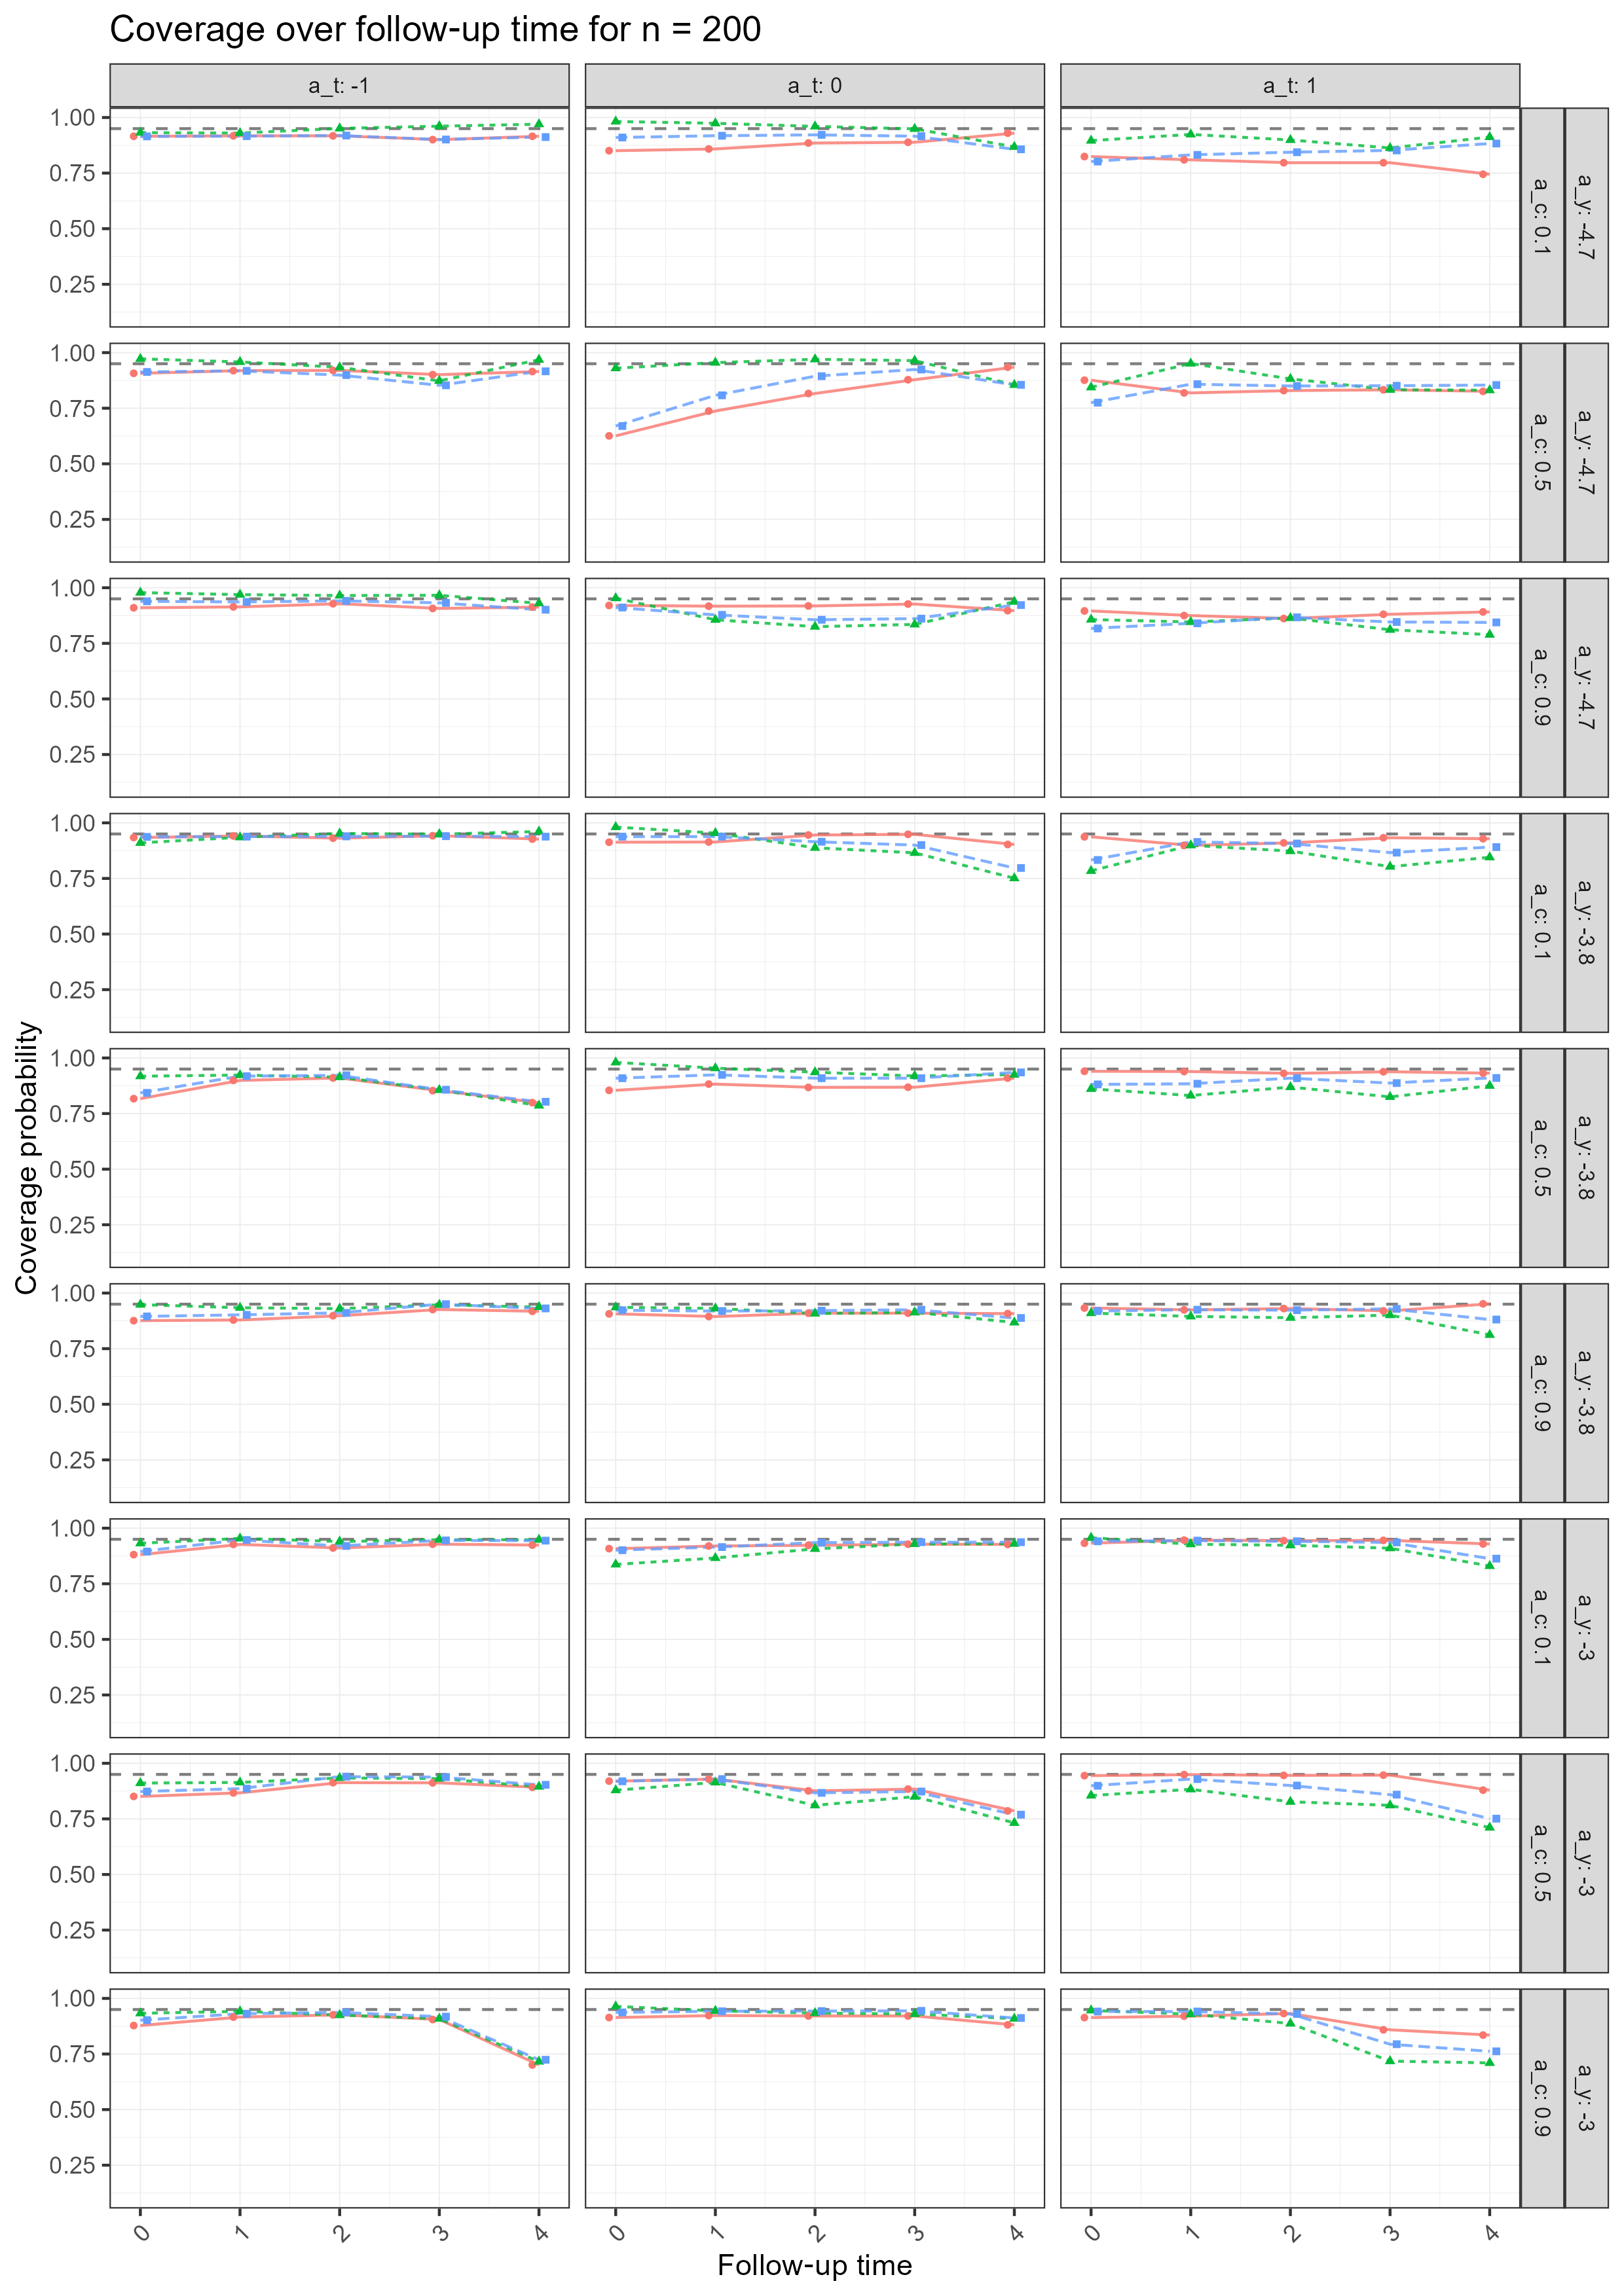
\includegraphics[height=0.95\textheight]{plots/plots_coverage200.png}
\caption{Coverage of the $95\%$ confidence interval over $1000$ simulations with sample size $n = 200$. The green line denotes \textcolor{green}{the empirical bootstrap CI}, the blue line denotes \textcolor{blue}{percentile bootstrap CI}, and the red line denotes \textcolor{red}{sandwich estimator CI}. The dashed gray line marks \textcolor{darkgray}{$95\%$}. The outcome event rate indicator is denoted by $a_y$, the confounding strength is denoted by $a_c$, and the treatment prevalence indicator is denoted by $a_t$.}\label{plt:coverage200}
\end{figure}

\newpage

\begin{figure}[H]
\centering
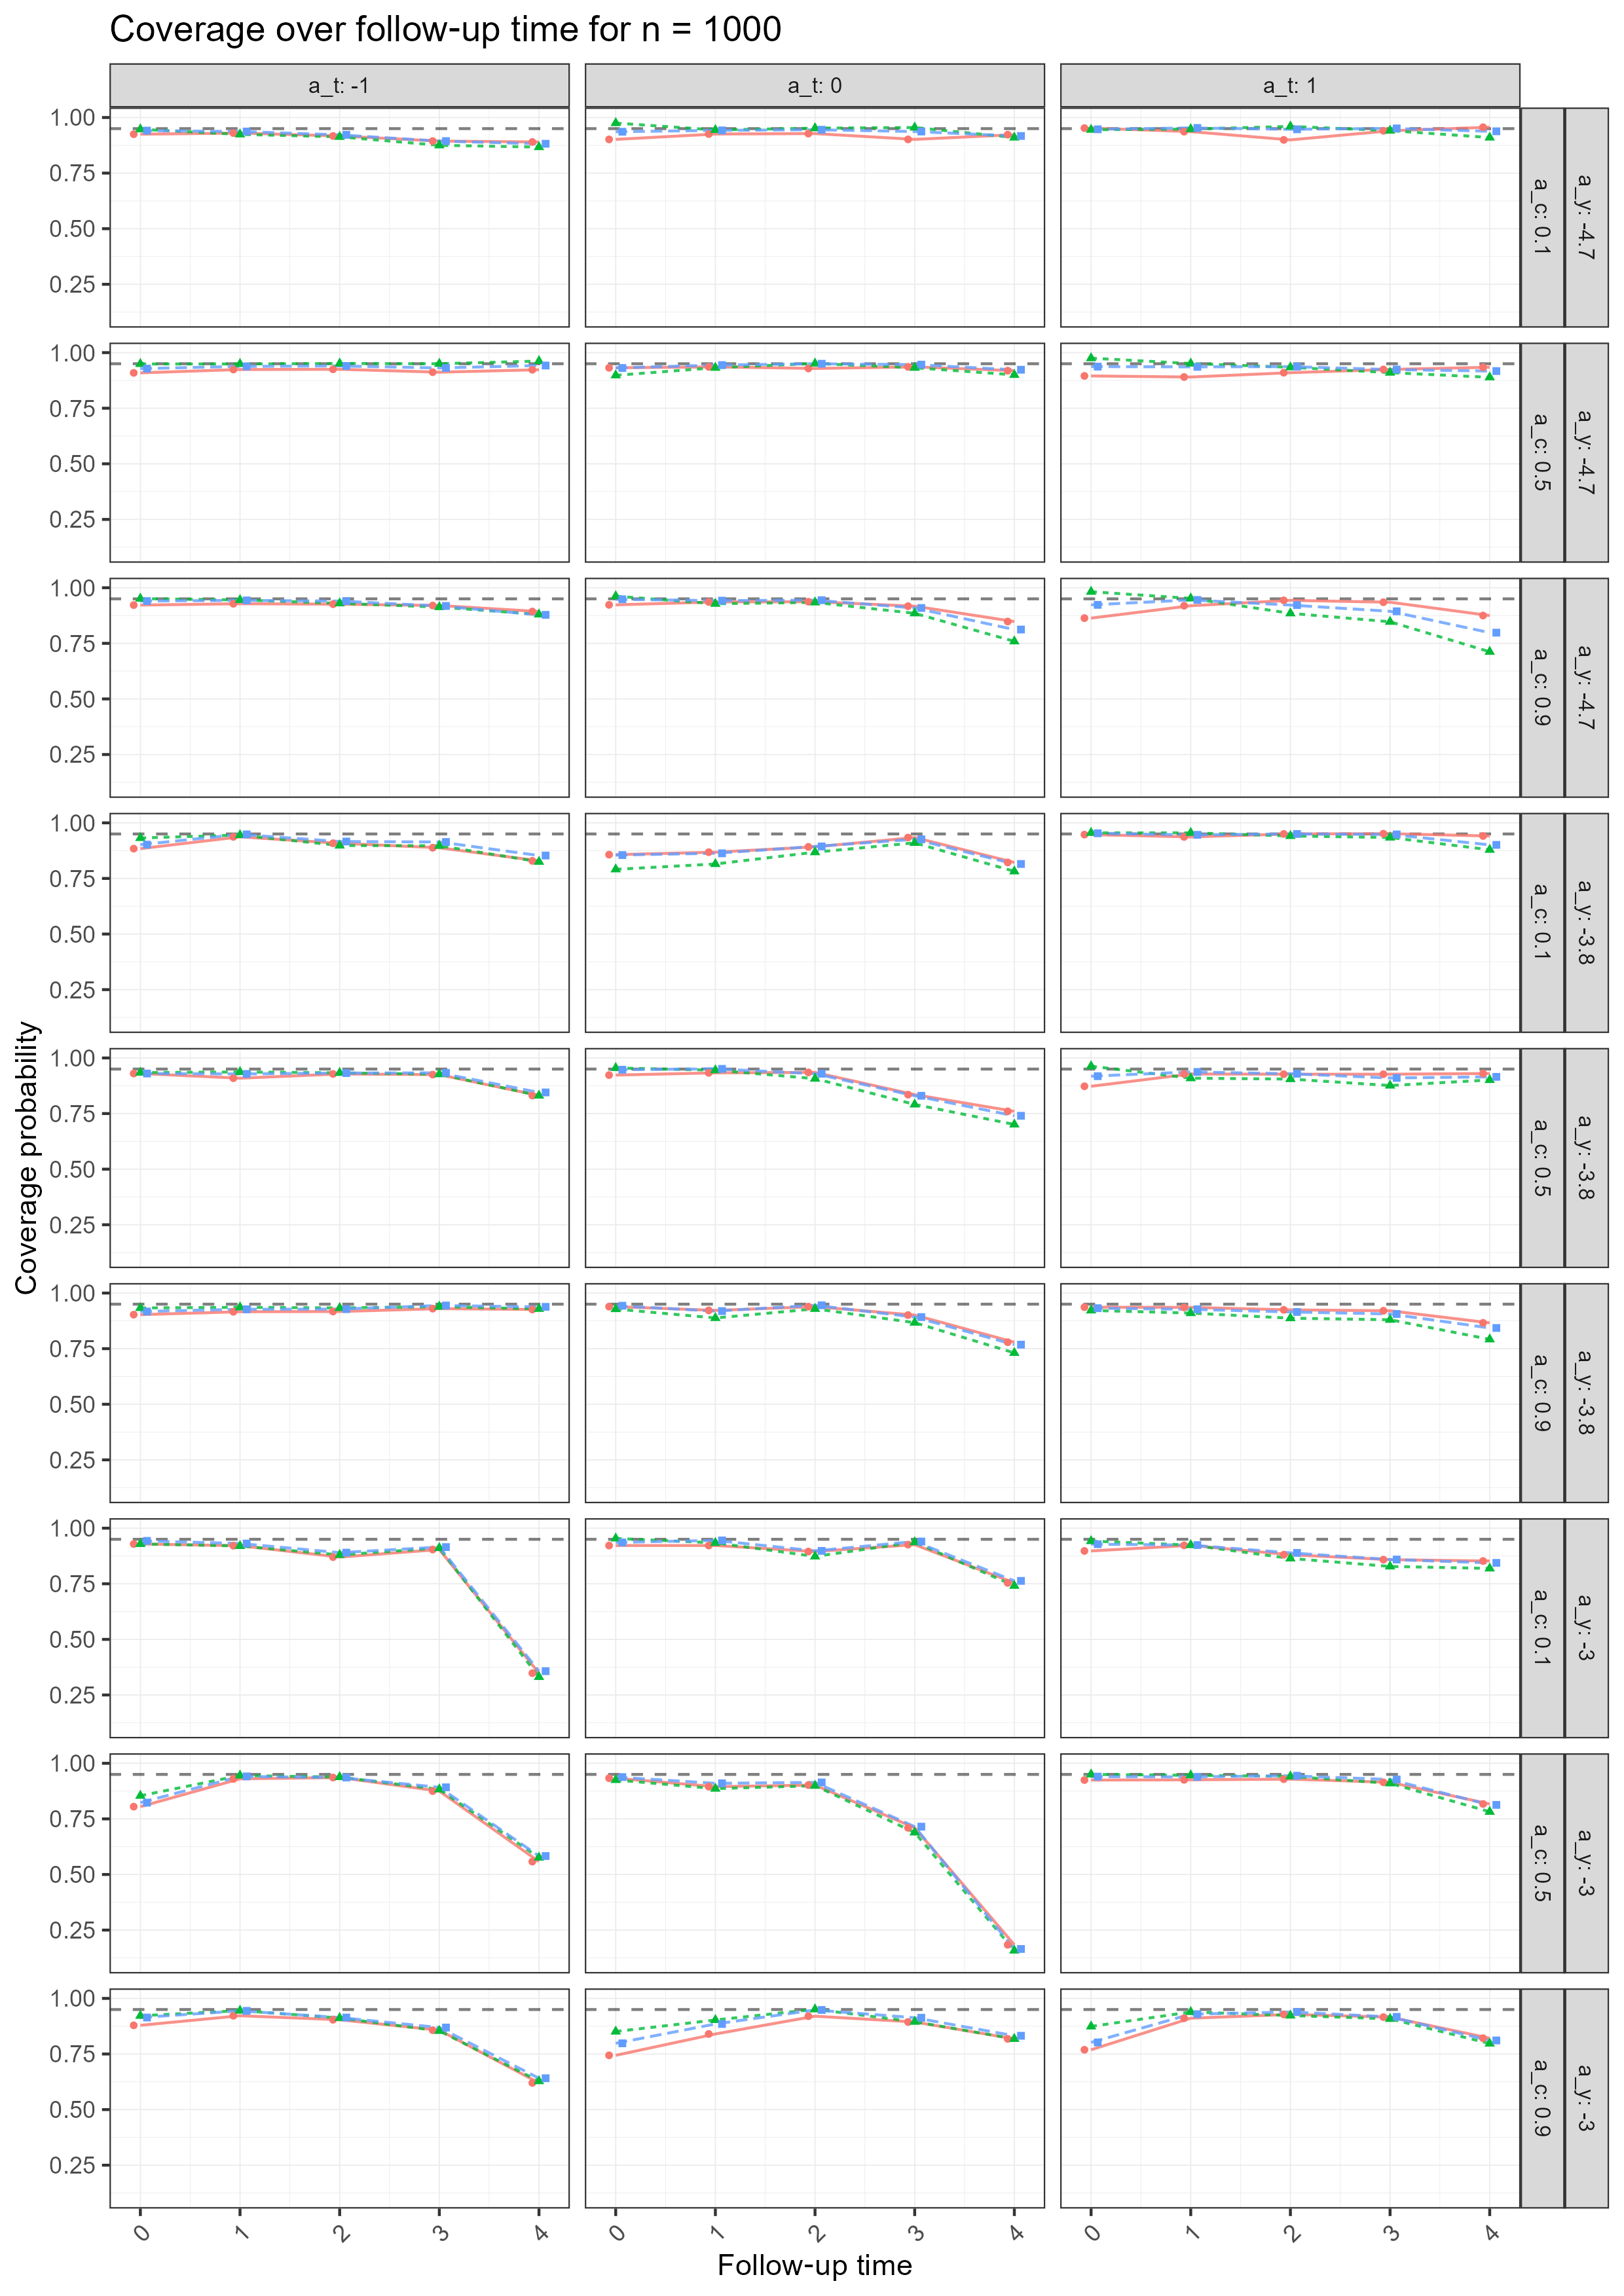
\includegraphics[height=0.95\textheight]{plots/plots_coverage1000.png}
\caption{Coverage of the $95\%$ confidence interval over $1000$ simulations with sample size $n = 1000$. The green line denotes \textcolor{green}{the empirical bootstrap CI}, the blue line denotes \textcolor{blue}{percentile bootstrap CI}, and the red line denotes \textcolor{red}{sandwich estimator CI}. The dashed gray line marks \textcolor{darkgray}{$95\%$}. The outcome event rate indicator is denoted by $a_y$, the confounding strength is denoted by $a_c$, and the treatment prevalence indicator is denoted by $a_t$.}\label{plt:coverage1000}
\end{figure}

\newpage

\begin{figure}[H]
\centering
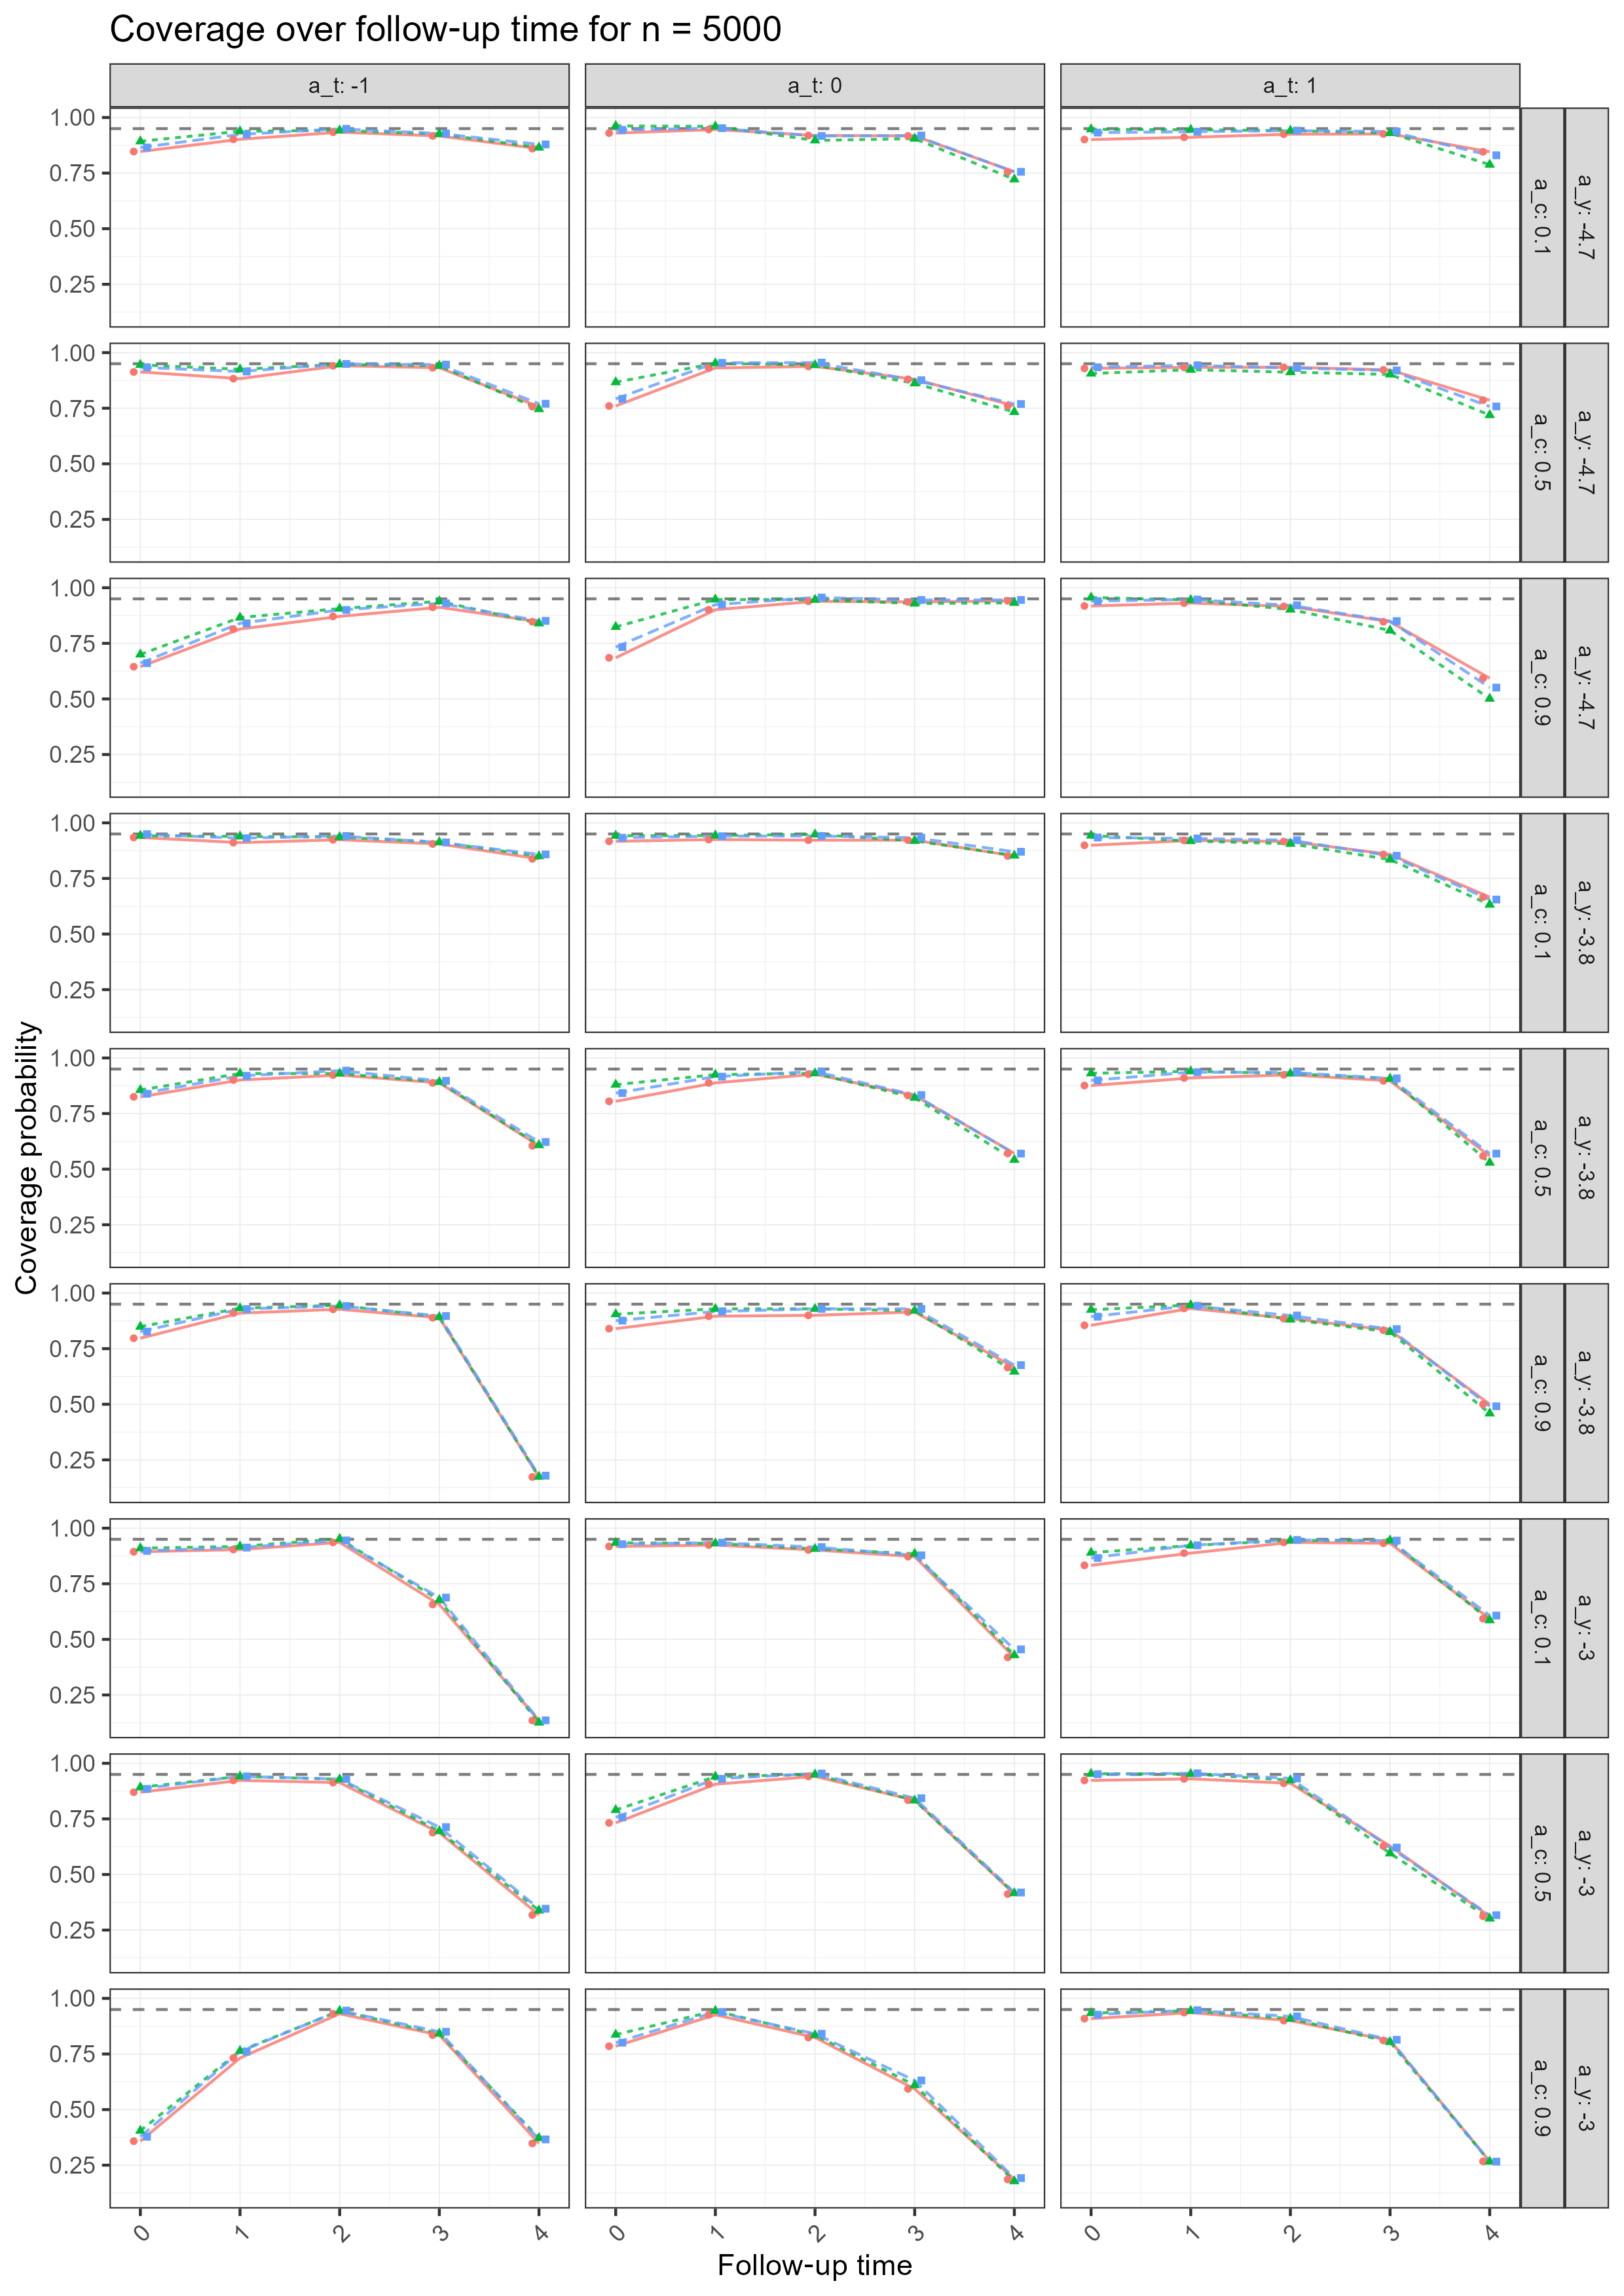
\includegraphics[height=0.95\textheight]{plots/plots_coverage5000.png}
\caption{Coverage of the $95\%$ confidence interval over $1000$ simulations with sample size $n = 5000$. The green line denotes \textcolor{green}{the empirical bootstrap CI}, the blue line denotes \textcolor{blue}{percentile bootstrap CI}, and the red line denotes \textcolor{red}{sandwich estimator CI}. The dashed gray line marks \textcolor{darkgray}{$95\%$}. The outcome event rate indicator is denoted by $a_y$, the confounding strength is denoted by $a_c$, and the treatment prevalence indicator is denoted by $a_t$.}\label{plt:coverage5000}
\end{figure}

\newpage

\begin{figure}[H]
\centering
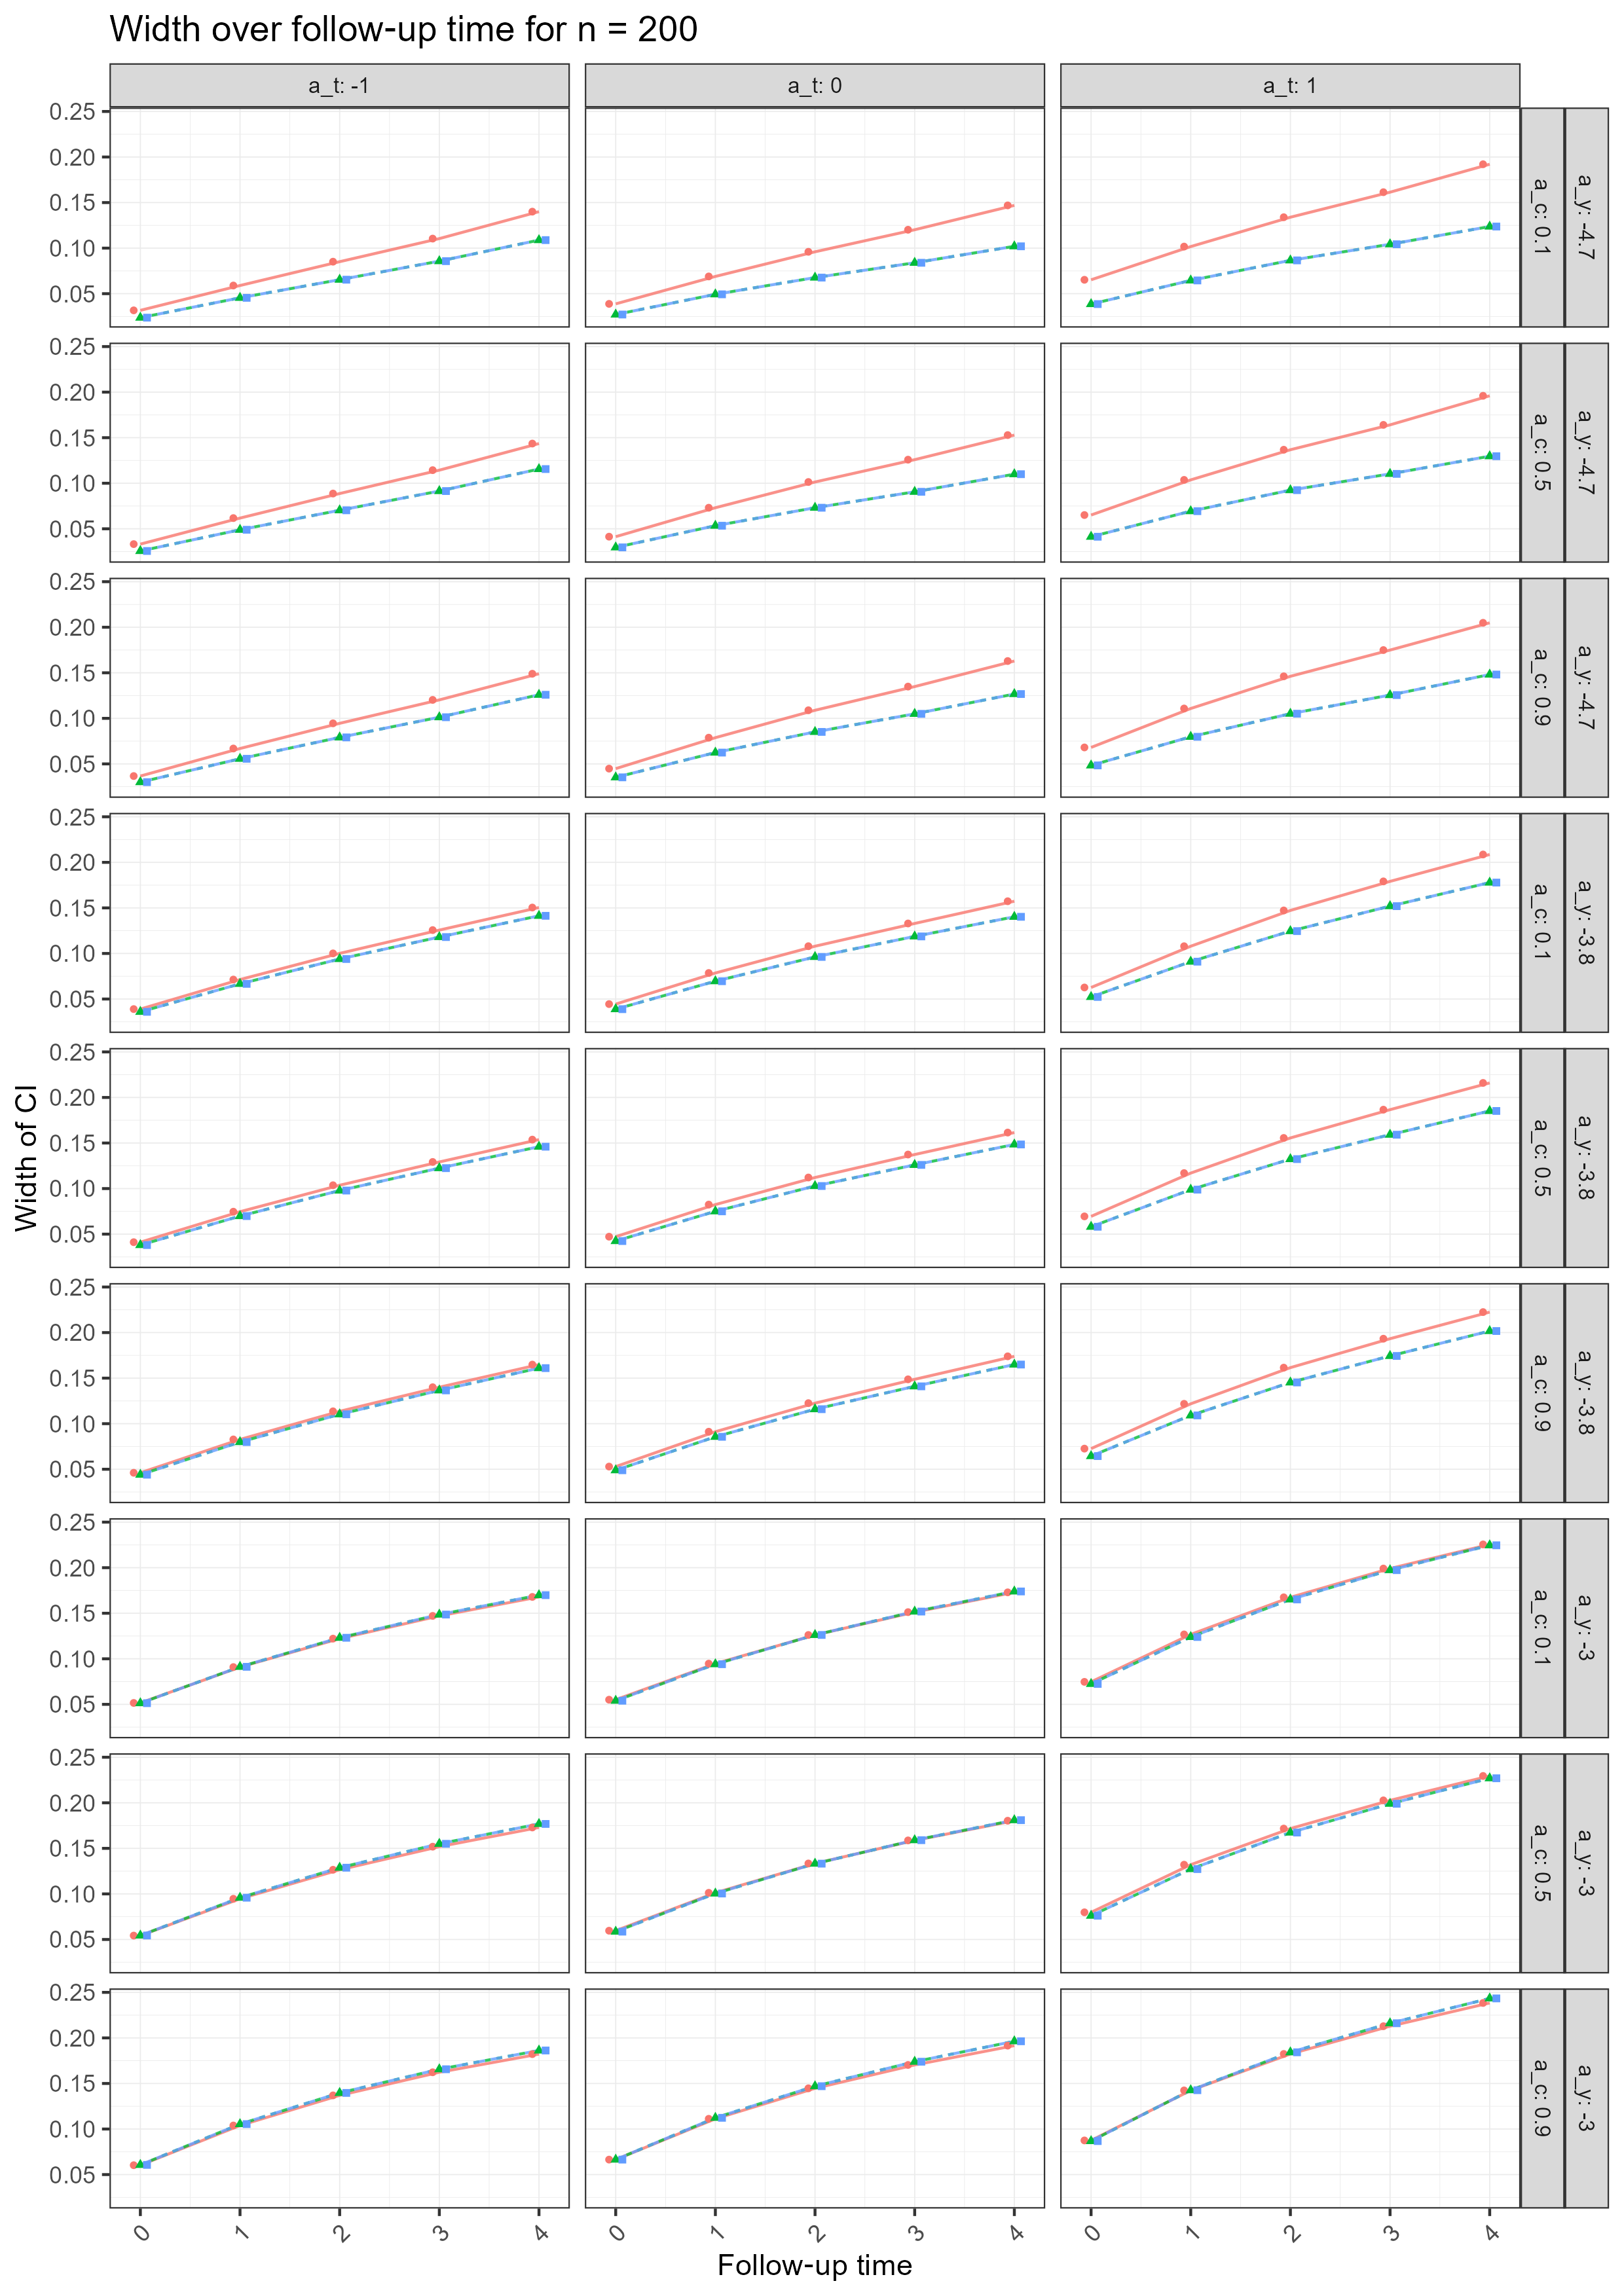
\includegraphics[height=0.95\textheight]{plots/plots_width200.png}
\caption{Width of the $95\%$ confidence interval over $1000$ simulations with sample size $n = 200$. The green line denotes \textcolor{green}{the empirical bootstrap CI}, the blue line denotes \textcolor{blue}{percentile bootstrap CI}, and the red line denotes \textcolor{red}{sandwich estimator CI}. The outcome event rate indicator is denoted by $a_y$, the confounding strength is denoted by $a_c$, and the treatment prevalence indicator is denoted by $a_t$.}\label{plt:width200}
\end{figure}

\newpage

\begin{figure}[H]
\centering
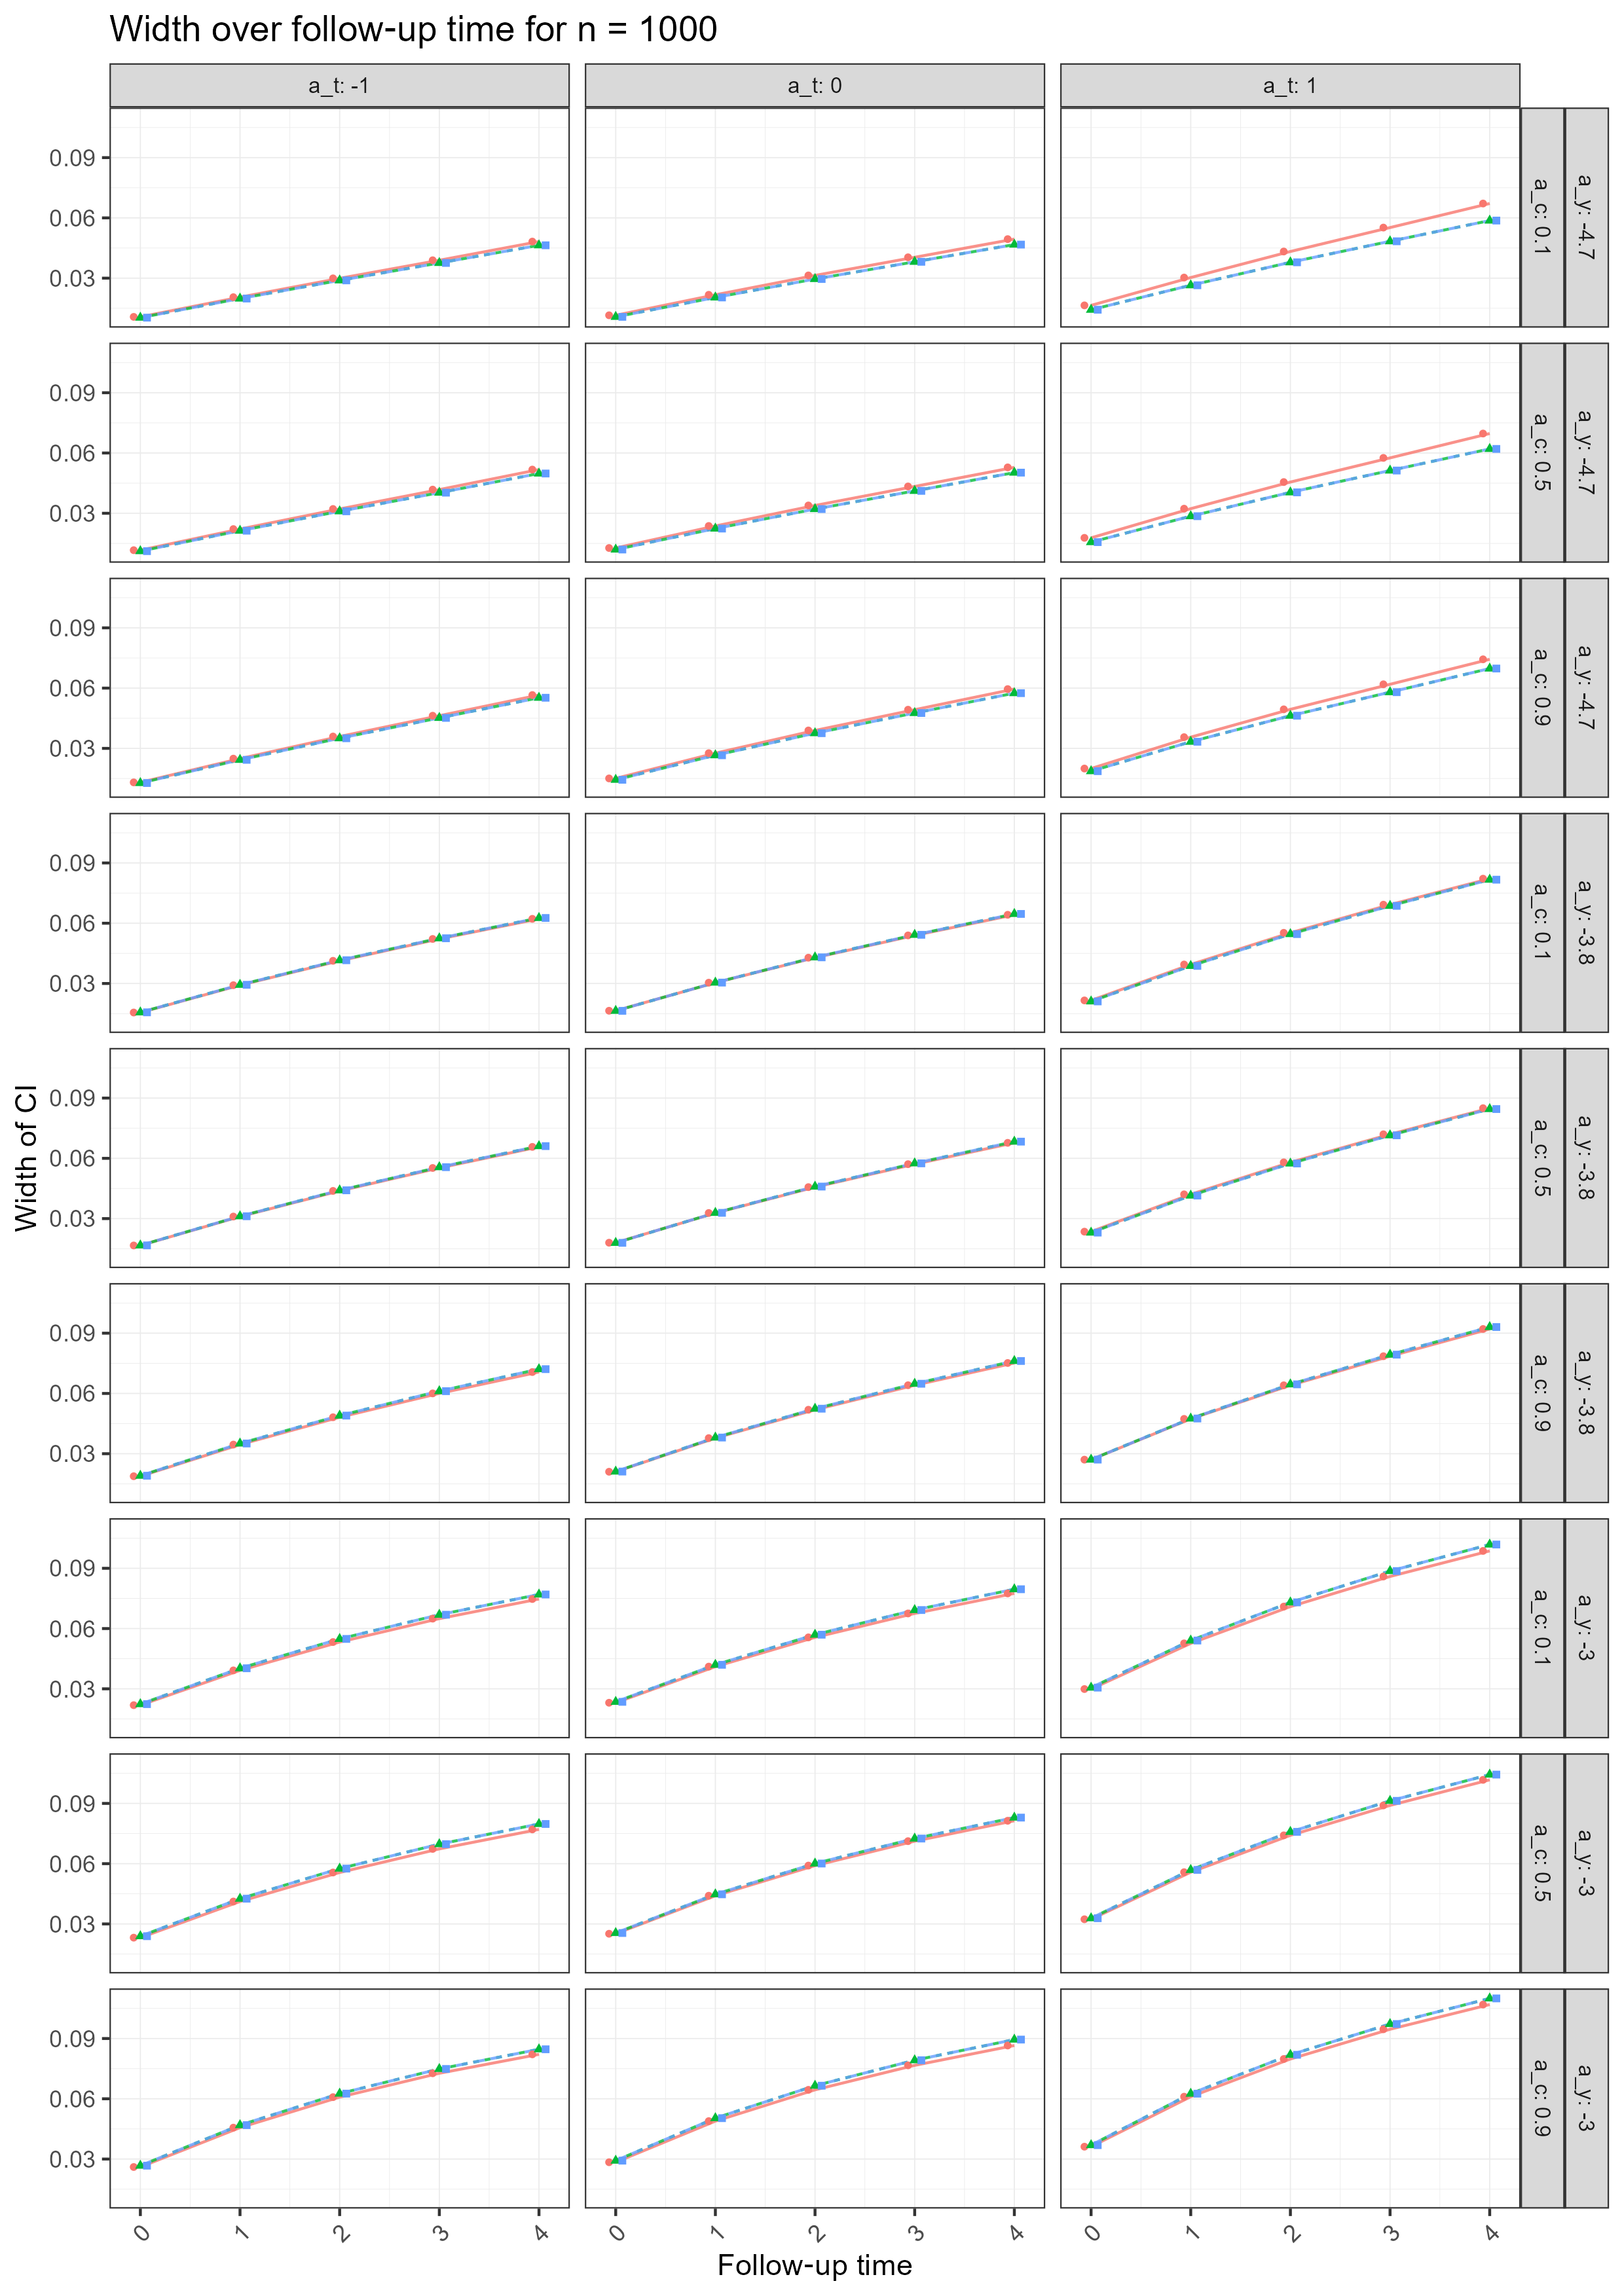
\includegraphics[height=0.95\textheight]{plots/plots_width1000.png}
\caption{Width of the $95\%$ confidence interval over $1000$ simulations with sample size $n = 1000$. The green line denotes \textcolor{green}{the empirical bootstrap CI}, the blue line denotes \textcolor{blue}{percentile bootstrap CI}, and the red line denotes \textcolor{red}{sandwich estimator CI}. The outcome event rate indicator is denoted by $a_y$, the confounding strength is denoted by $a_c$, and the treatment prevalence indicator is denoted by $a_t$.}\label{plt:width1000}
\end{figure}

\newpage

\begin{figure}[H]
\centering
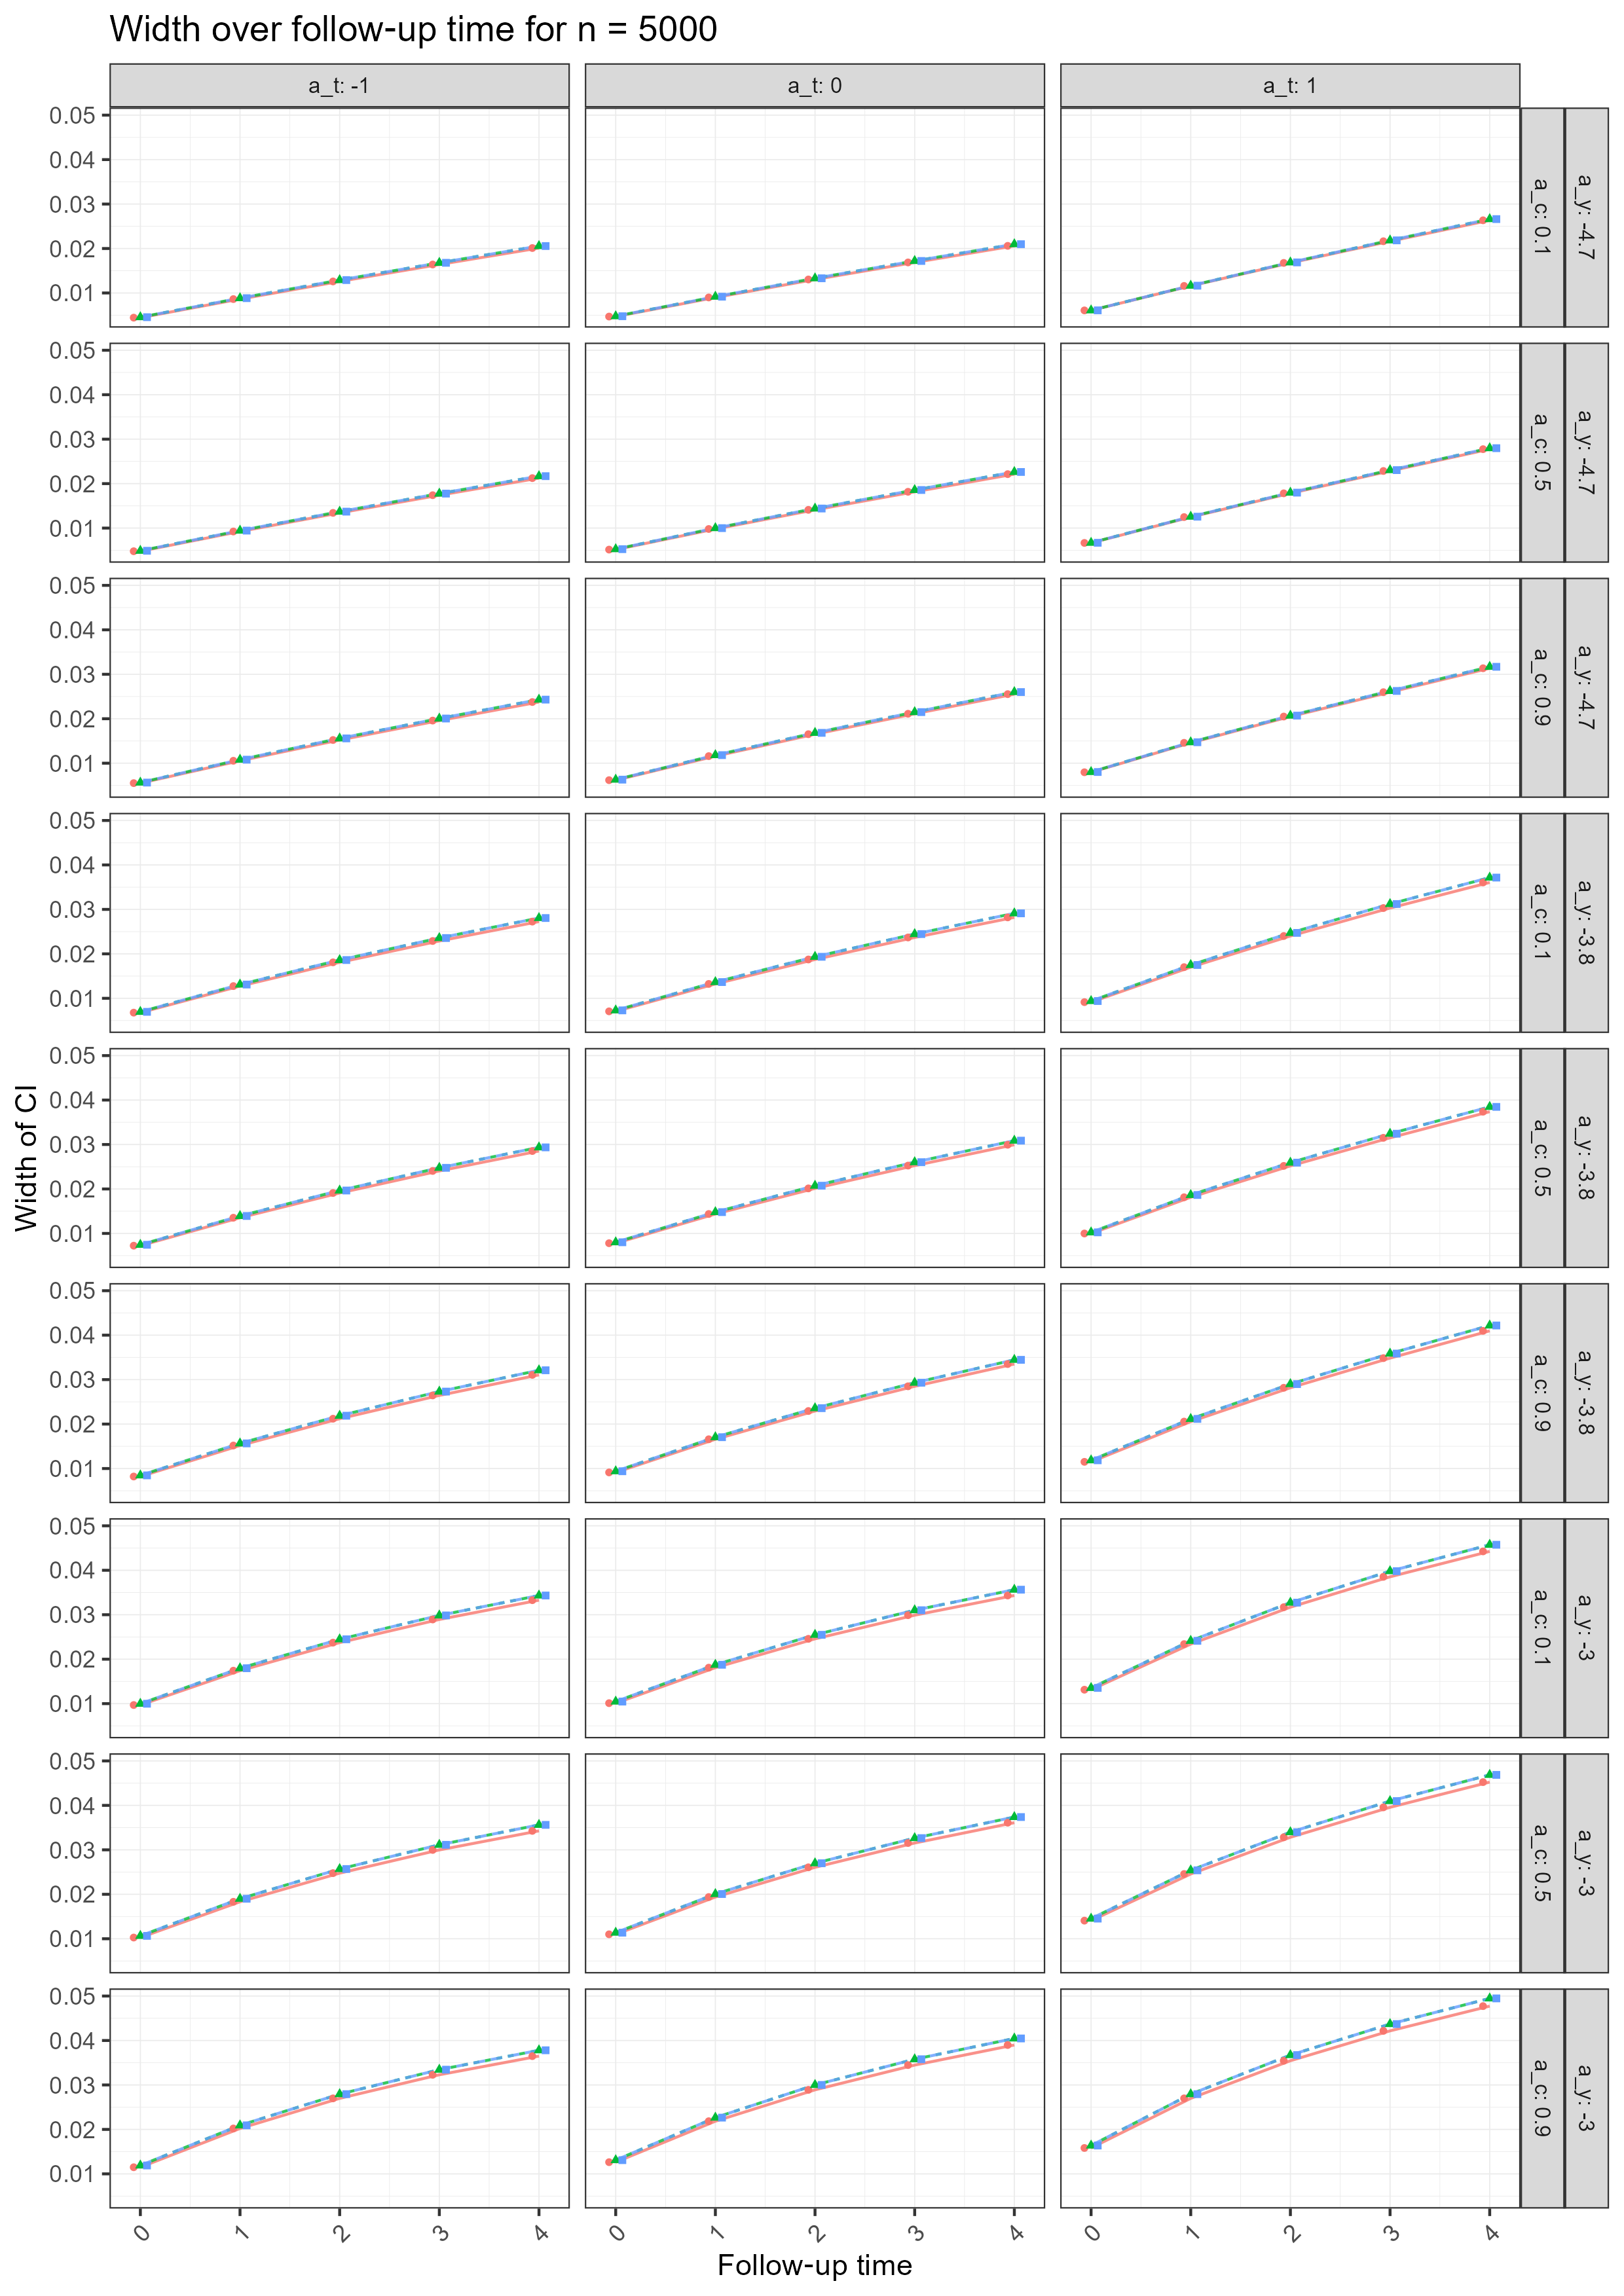
\includegraphics[height=0.95\textheight]{plots/plots_width5000.png}
\caption{Width of the $95\%$ confidence interval over $1000$ simulations with sample size $n = 5000$. The green line denotes \textcolor{green}{the empirical bootstrap CI}, the blue line denotes \textcolor{blue}{percentile bootstrap CI}, and the red line denotes \textcolor{red}{sandwich estimator CI}. The outcome event rate indicator is denoted by $a_y$, the confounding strength is denoted by $a_c$, and the treatment prevalence indicator is denoted by $a_t$.}\label{plt:width5000}
\end{figure}

\newpage

\begin{figure}[H]
\centering
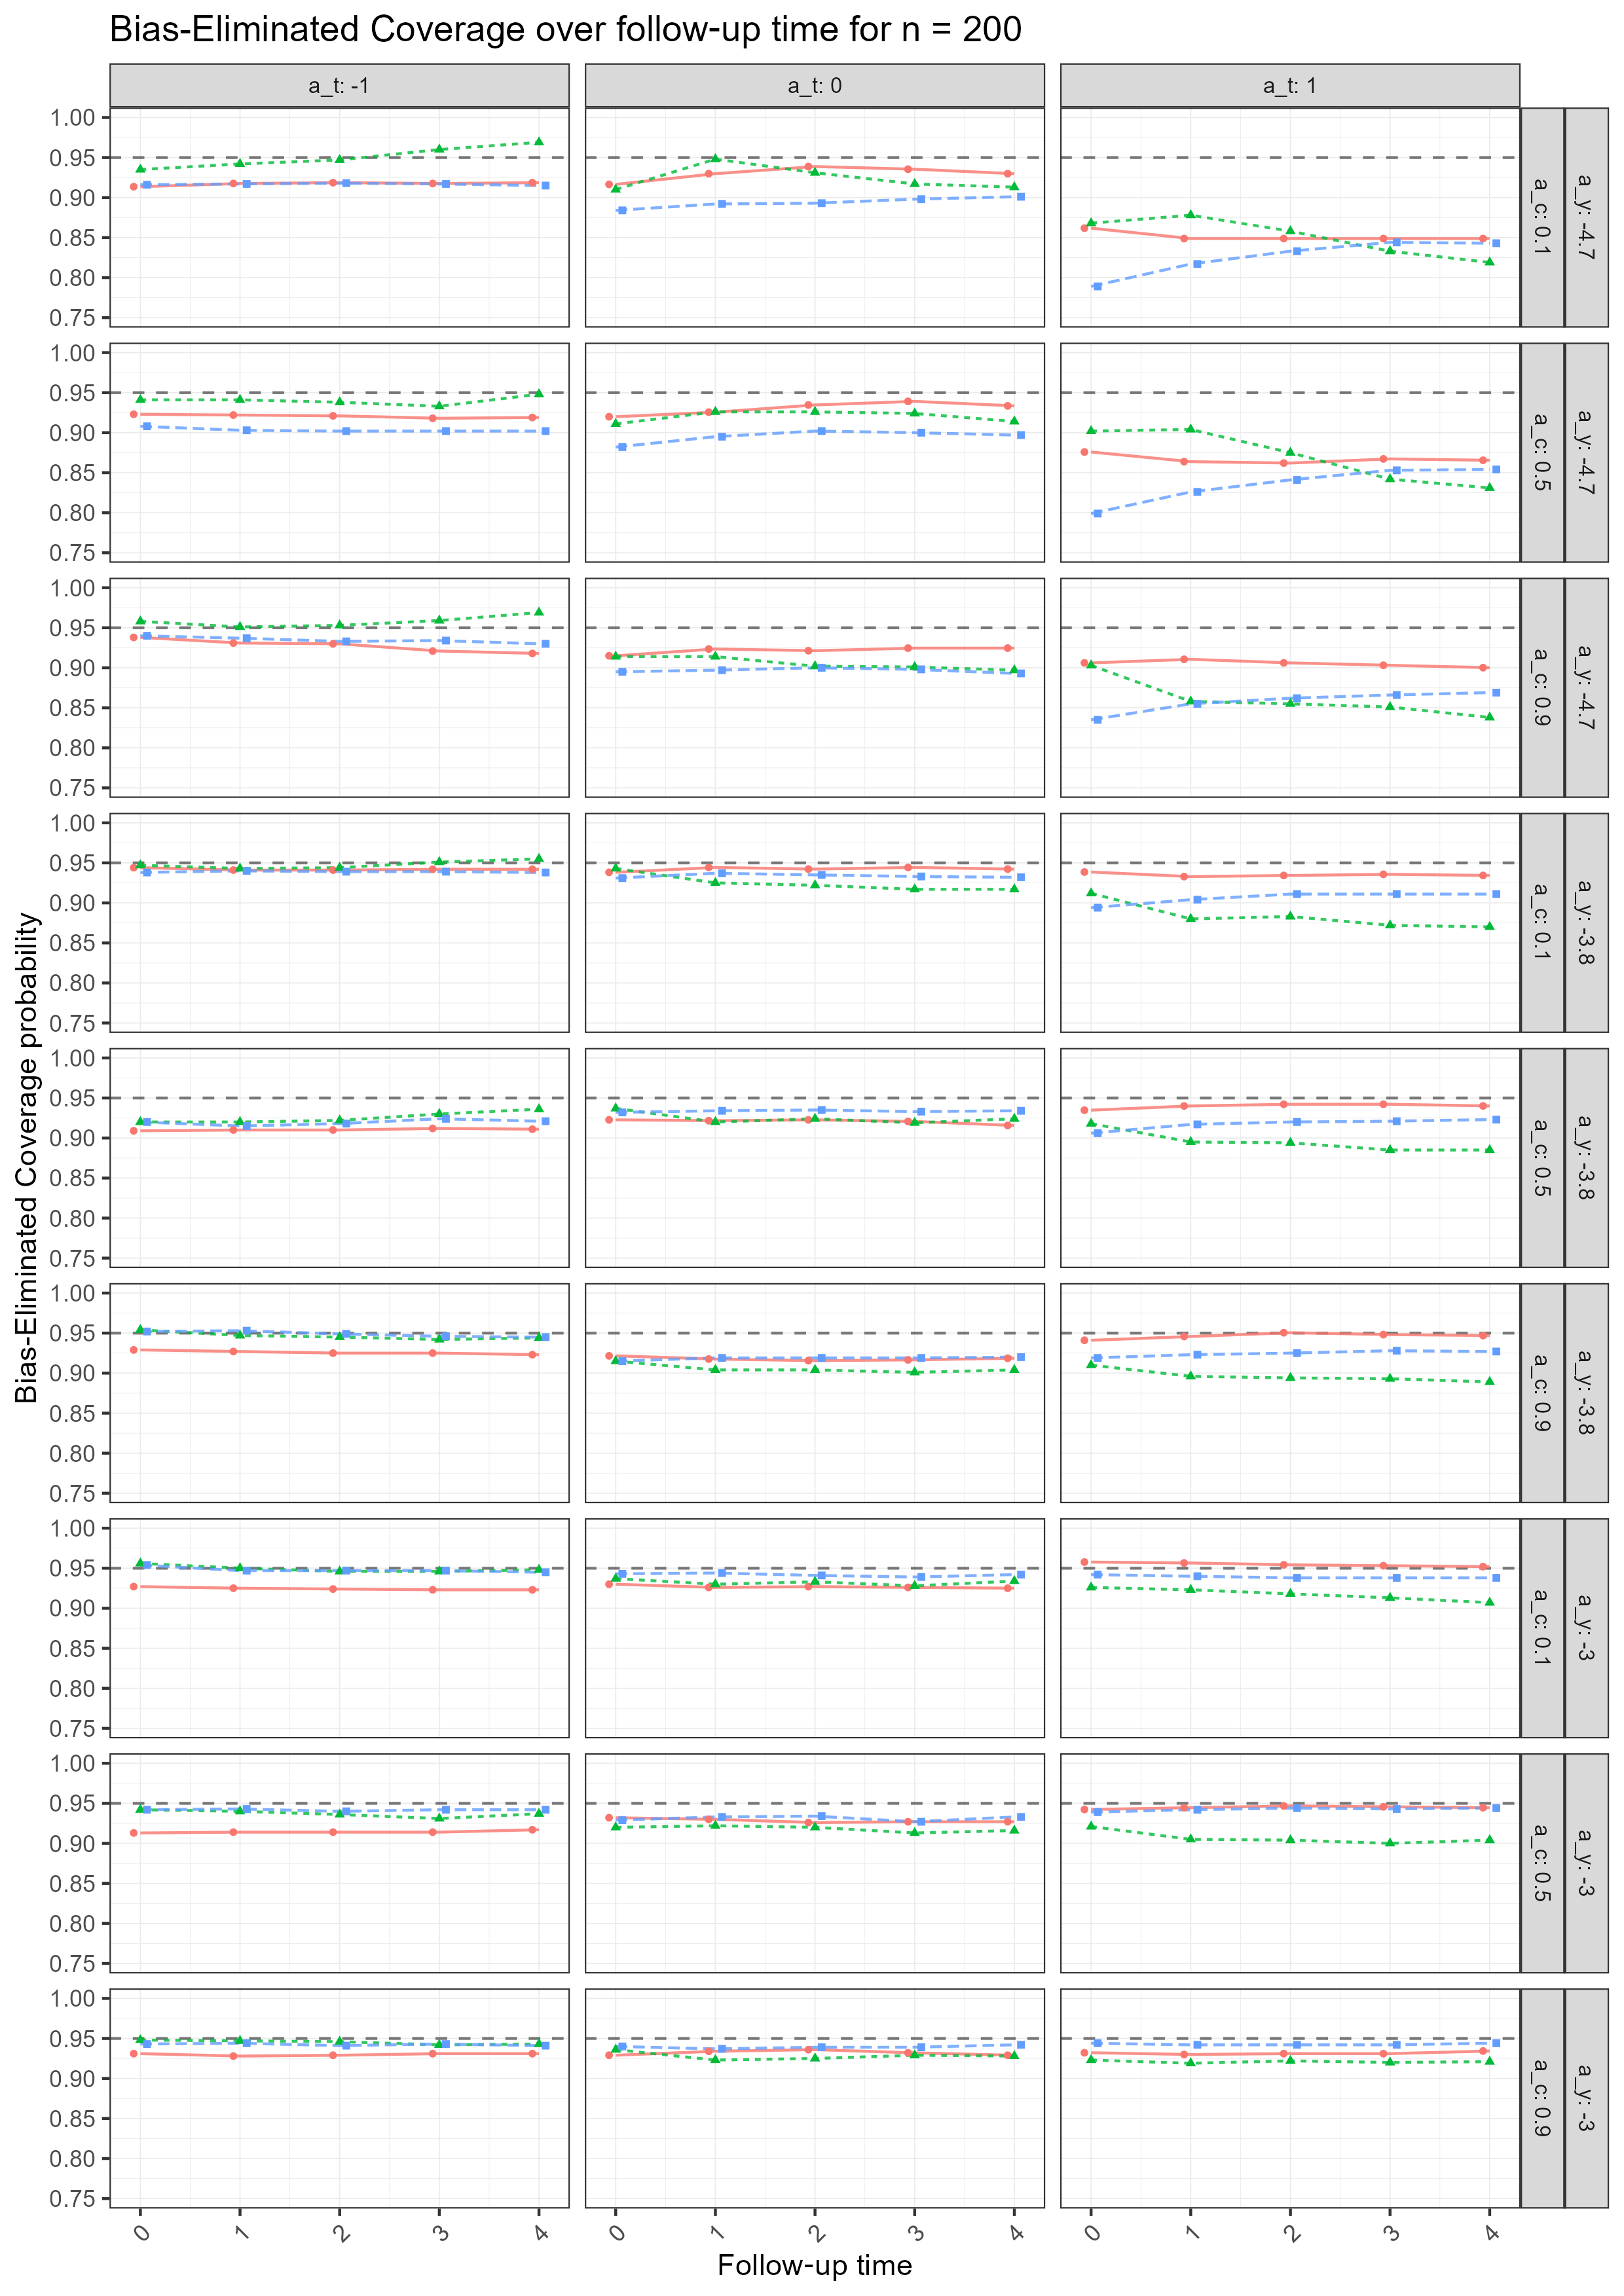
\includegraphics[height=0.95\textheight]{plots/plots_bias_coverage200.png}
\caption{Bias-eliminated coverage of the $95\%$ confidence interval over $1000$ simulations with sample size $n = 200$. The green line denotes \textcolor{green}{the empirical bootstrap CI}, the blue line denotes \textcolor{blue}{percentile bootstrap CI}, and the red line denotes \textcolor{red}{sandwich estimator CI}. The dashed gray line marks \textcolor{darkgray}{$95\%$}. The outcome event rate indicator is denoted by $a_y$, the confounding strength is denoted by $a_c$, and the treatment prevalence indicator is denoted by $a_t$.}\label{plt:biascoverage200}
\end{figure}

\newpage

\begin{figure}[H]
\centering
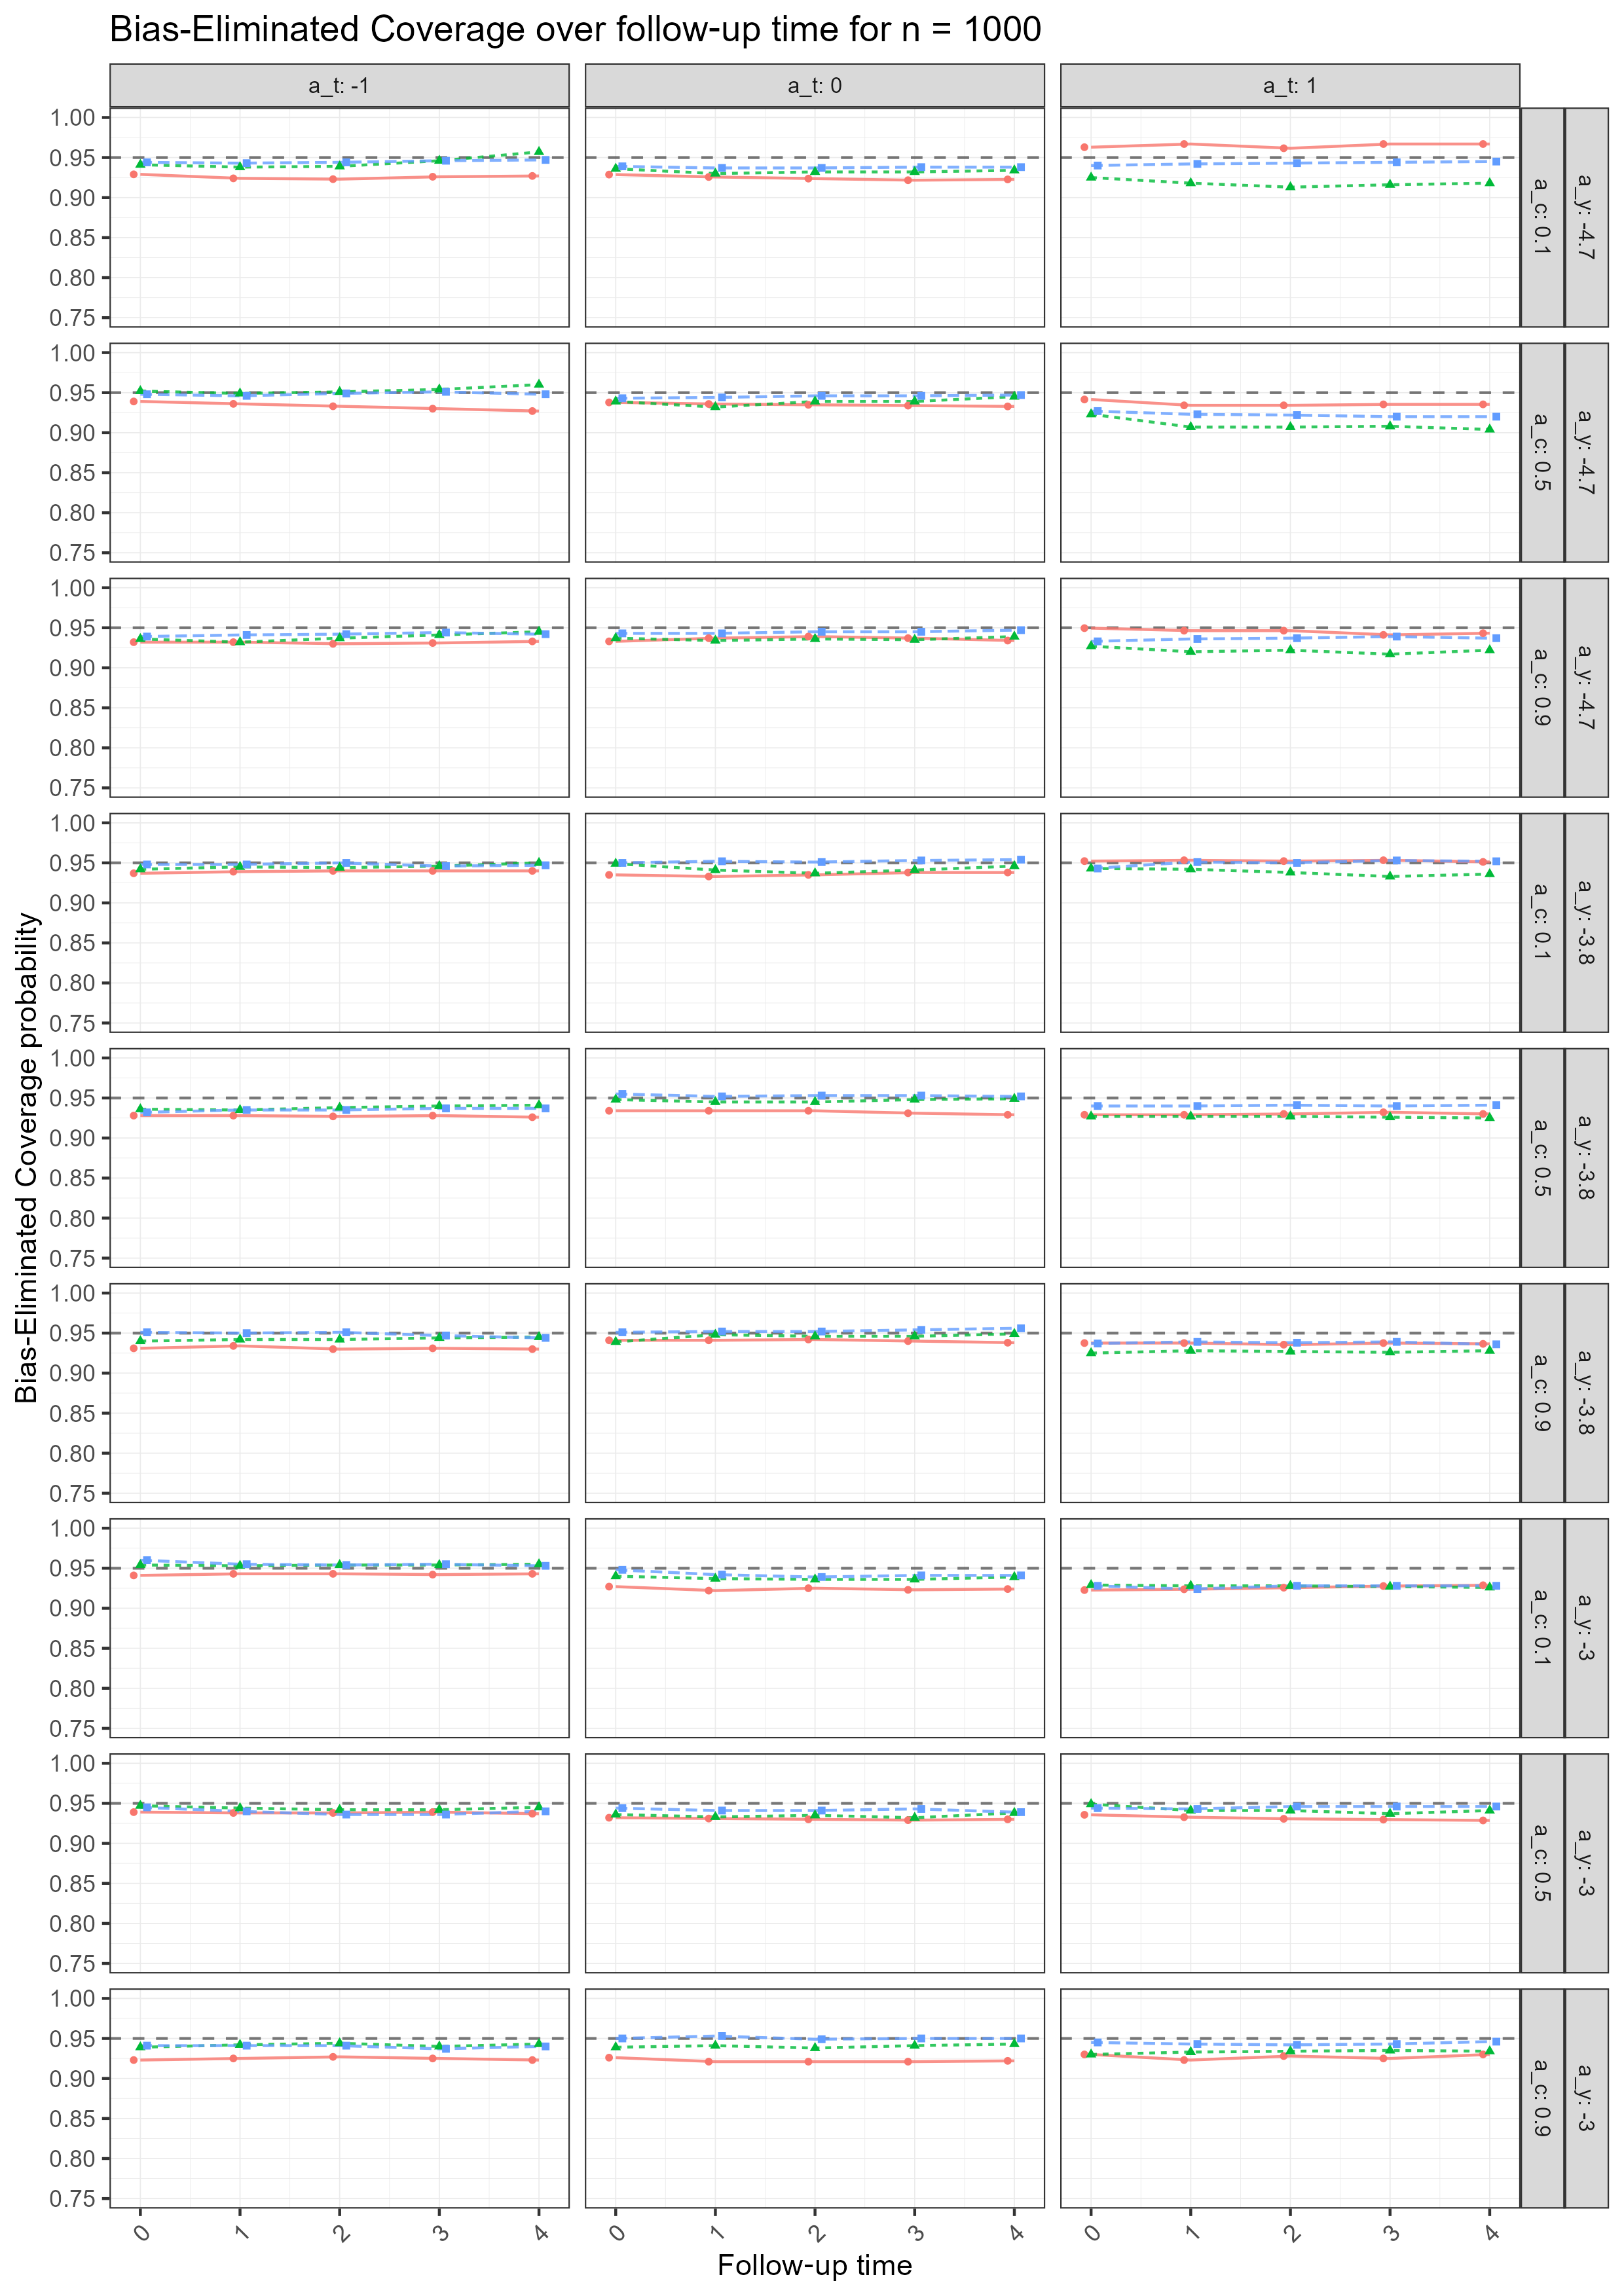
\includegraphics[height=0.95\textheight]{plots/plots_bias_coverage1000.png}
\caption{Bias-eliminated coverage of the $95\%$ confidence interval over $1000$ simulations with sample size $n = 1000$. The green line denotes \textcolor{green}{the empirical bootstrap CI}, the blue line denotes \textcolor{blue}{percentile bootstrap CI}, and the red line denotes \textcolor{red}{sandwich estimator CI}. The dashed gray line marks \textcolor{darkgray}{$95\%$}. The outcome event rate indicator is denoted by $a_y$, the confounding strength is denoted by $a_c$, and the treatment prevalence indicator is denoted by $a_t$.}\label{plt:biascoverage1000}
\end{figure}

\newpage

\begin{figure}[H]
\centering
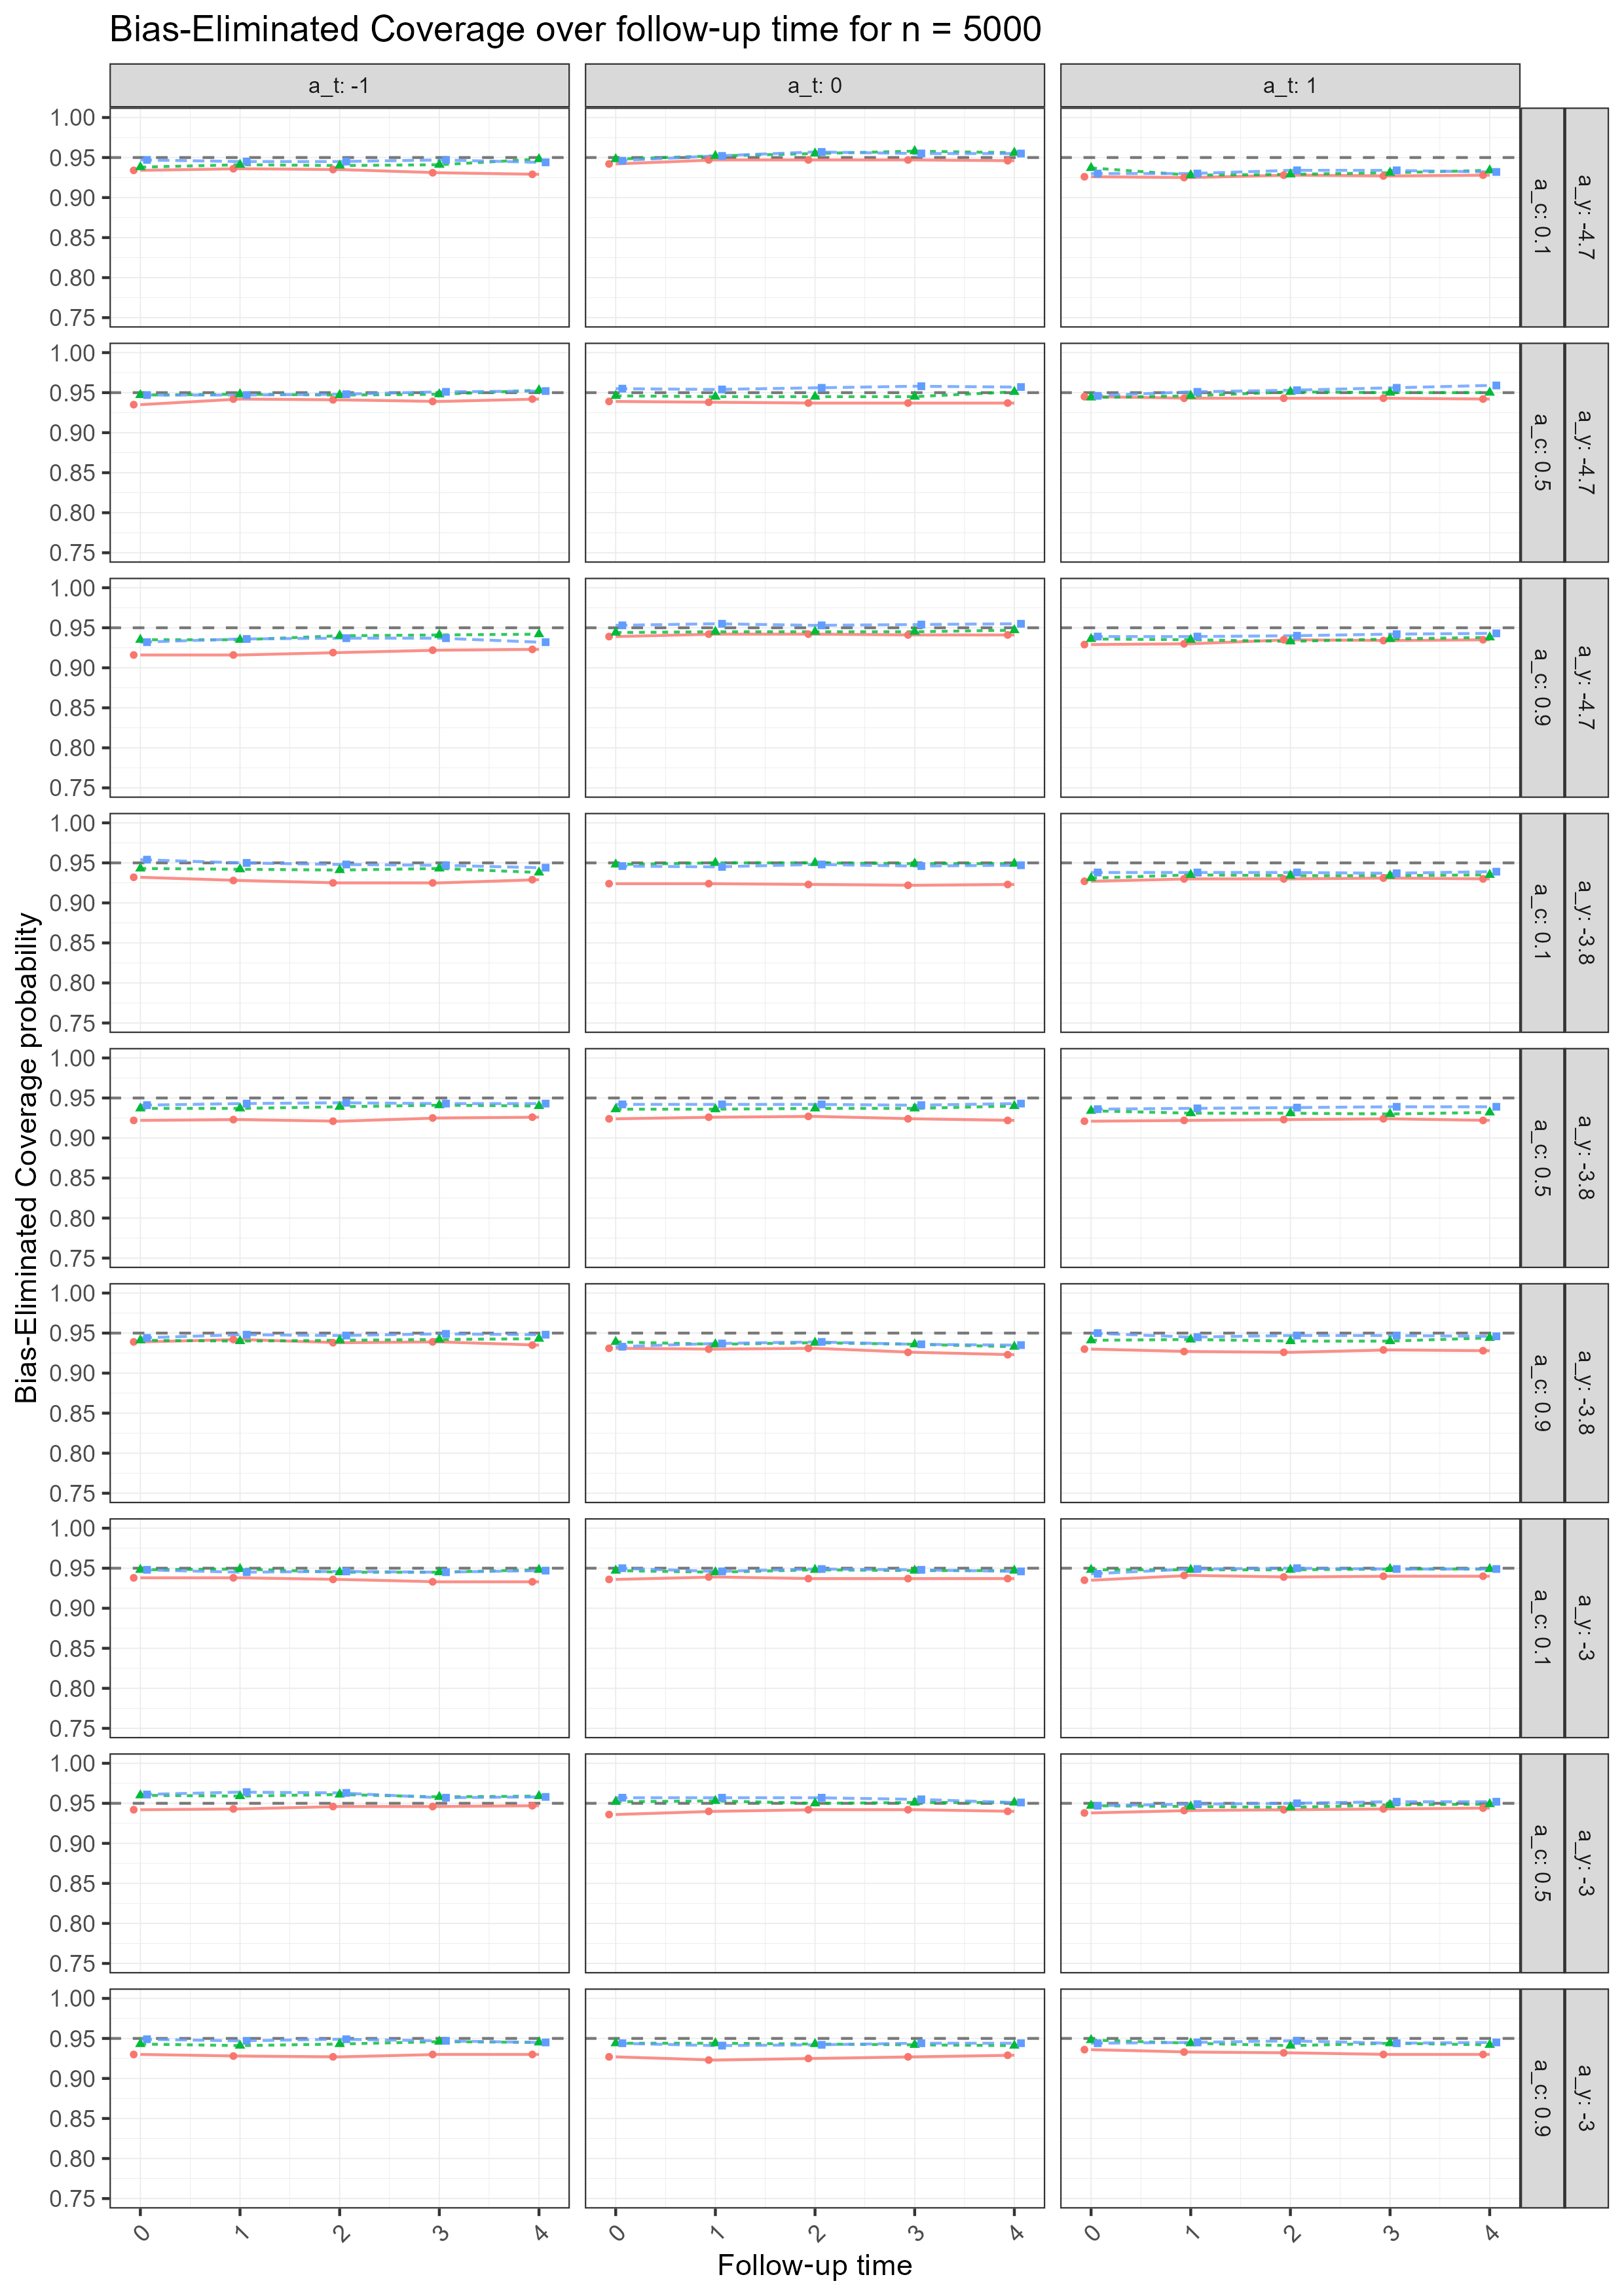
\includegraphics[height=0.95\textheight]{plots/plots_bias_coverage5000.png}
\caption{Bias-eliminated coverage of the $95\%$ confidence interval over $1000$ simulations with sample size $n = 5000$. The green line denotes \textcolor{green}{the empirical bootstrap CI}, the blue line denotes \textcolor{blue}{percentile bootstrap CI}, and the red line denotes \textcolor{red}{sandwich estimator CI}. The dashed gray line marks \textcolor{darkgray}{$95\%$}. The outcome event rate indicator is denoted by $a_y$, the confounding strength is denoted by $a_c$, and the treatment prevalence indicator is denoted by $a_t$.}\label{plt:biascoverage5000}
\end{figure}

\newpage

\begin{figure}[H]
\centering
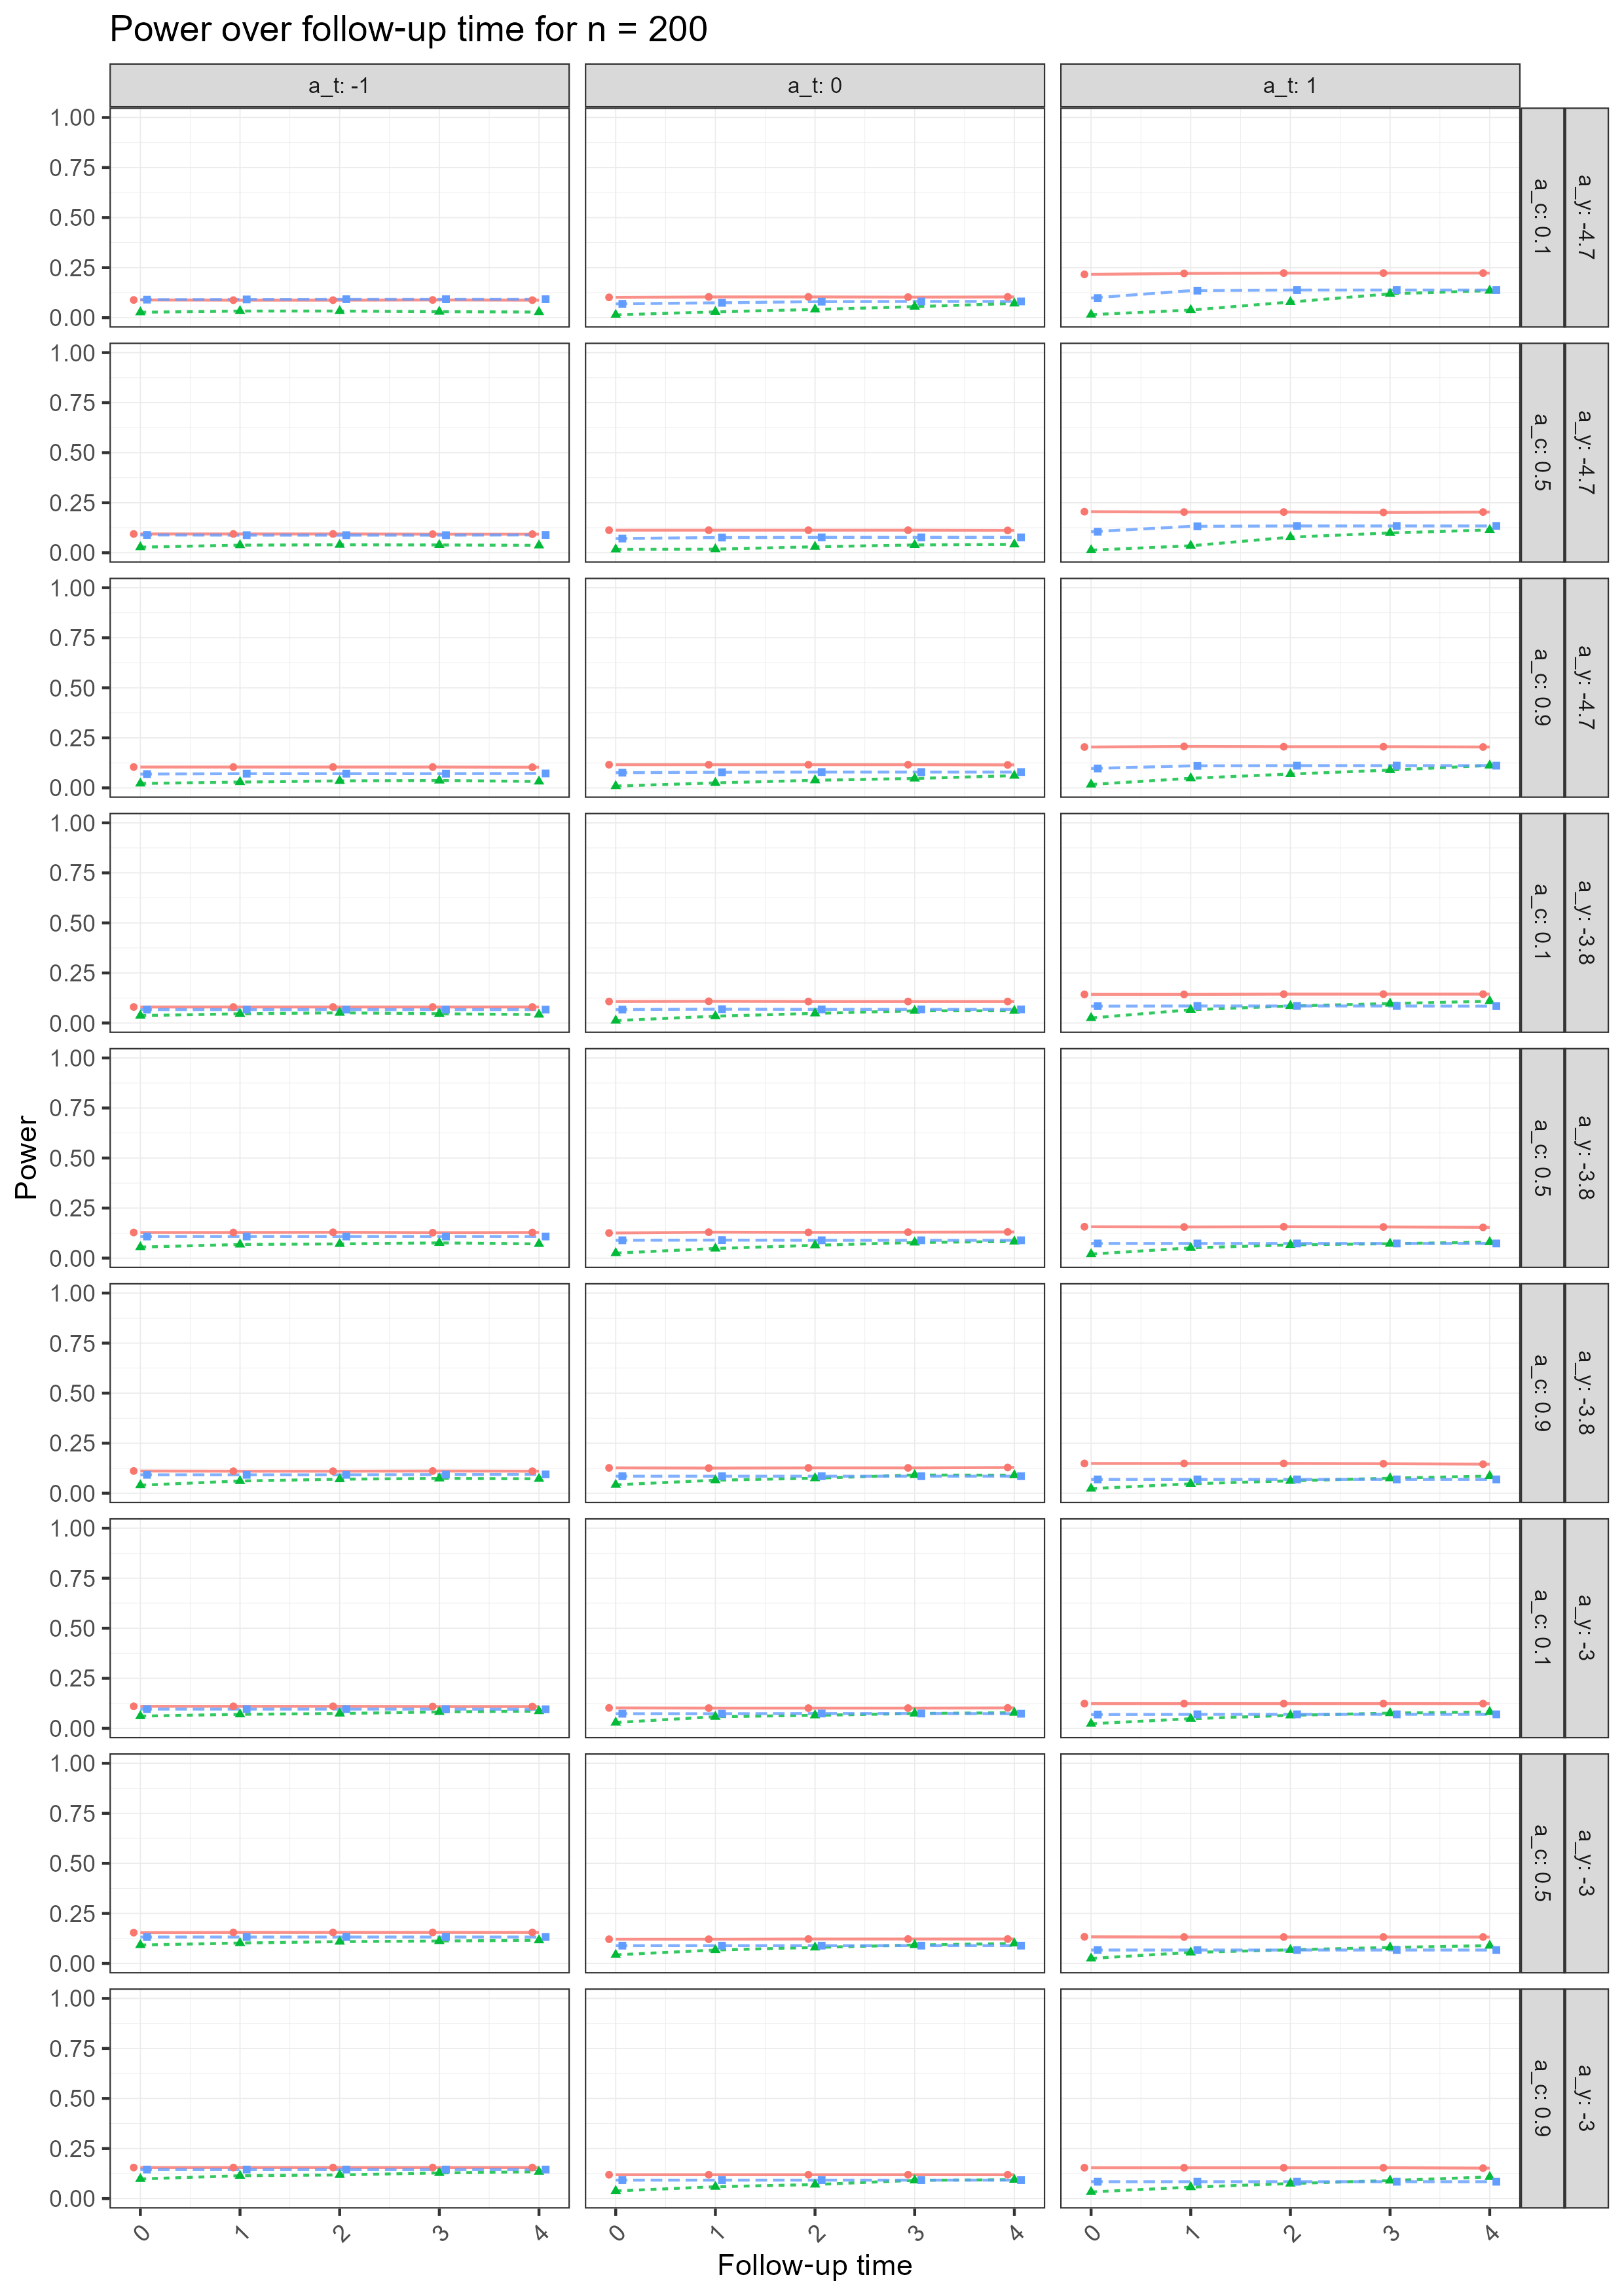
\includegraphics[height=0.95\textheight]{plots/plots_power200.png}
\caption{Power of the $95\%$ confidence interval over $1000$ simulations with sample size $n = 200$. The green line denotes \textcolor{green}{the empirical bootstrap CI}, the blue line denotes \textcolor{blue}{percentile bootstrap CI}, and the red line denotes \textcolor{red}{sandwich estimator CI}. The outcome event rate indicator is denoted by $a_y$, the confounding strength is denoted by $a_c$, and the treatment prevalence indicator is denoted by $a_t$.}
\label{plt:power200}
\end{figure}

\newpage

\begin{figure}[H]
\centering
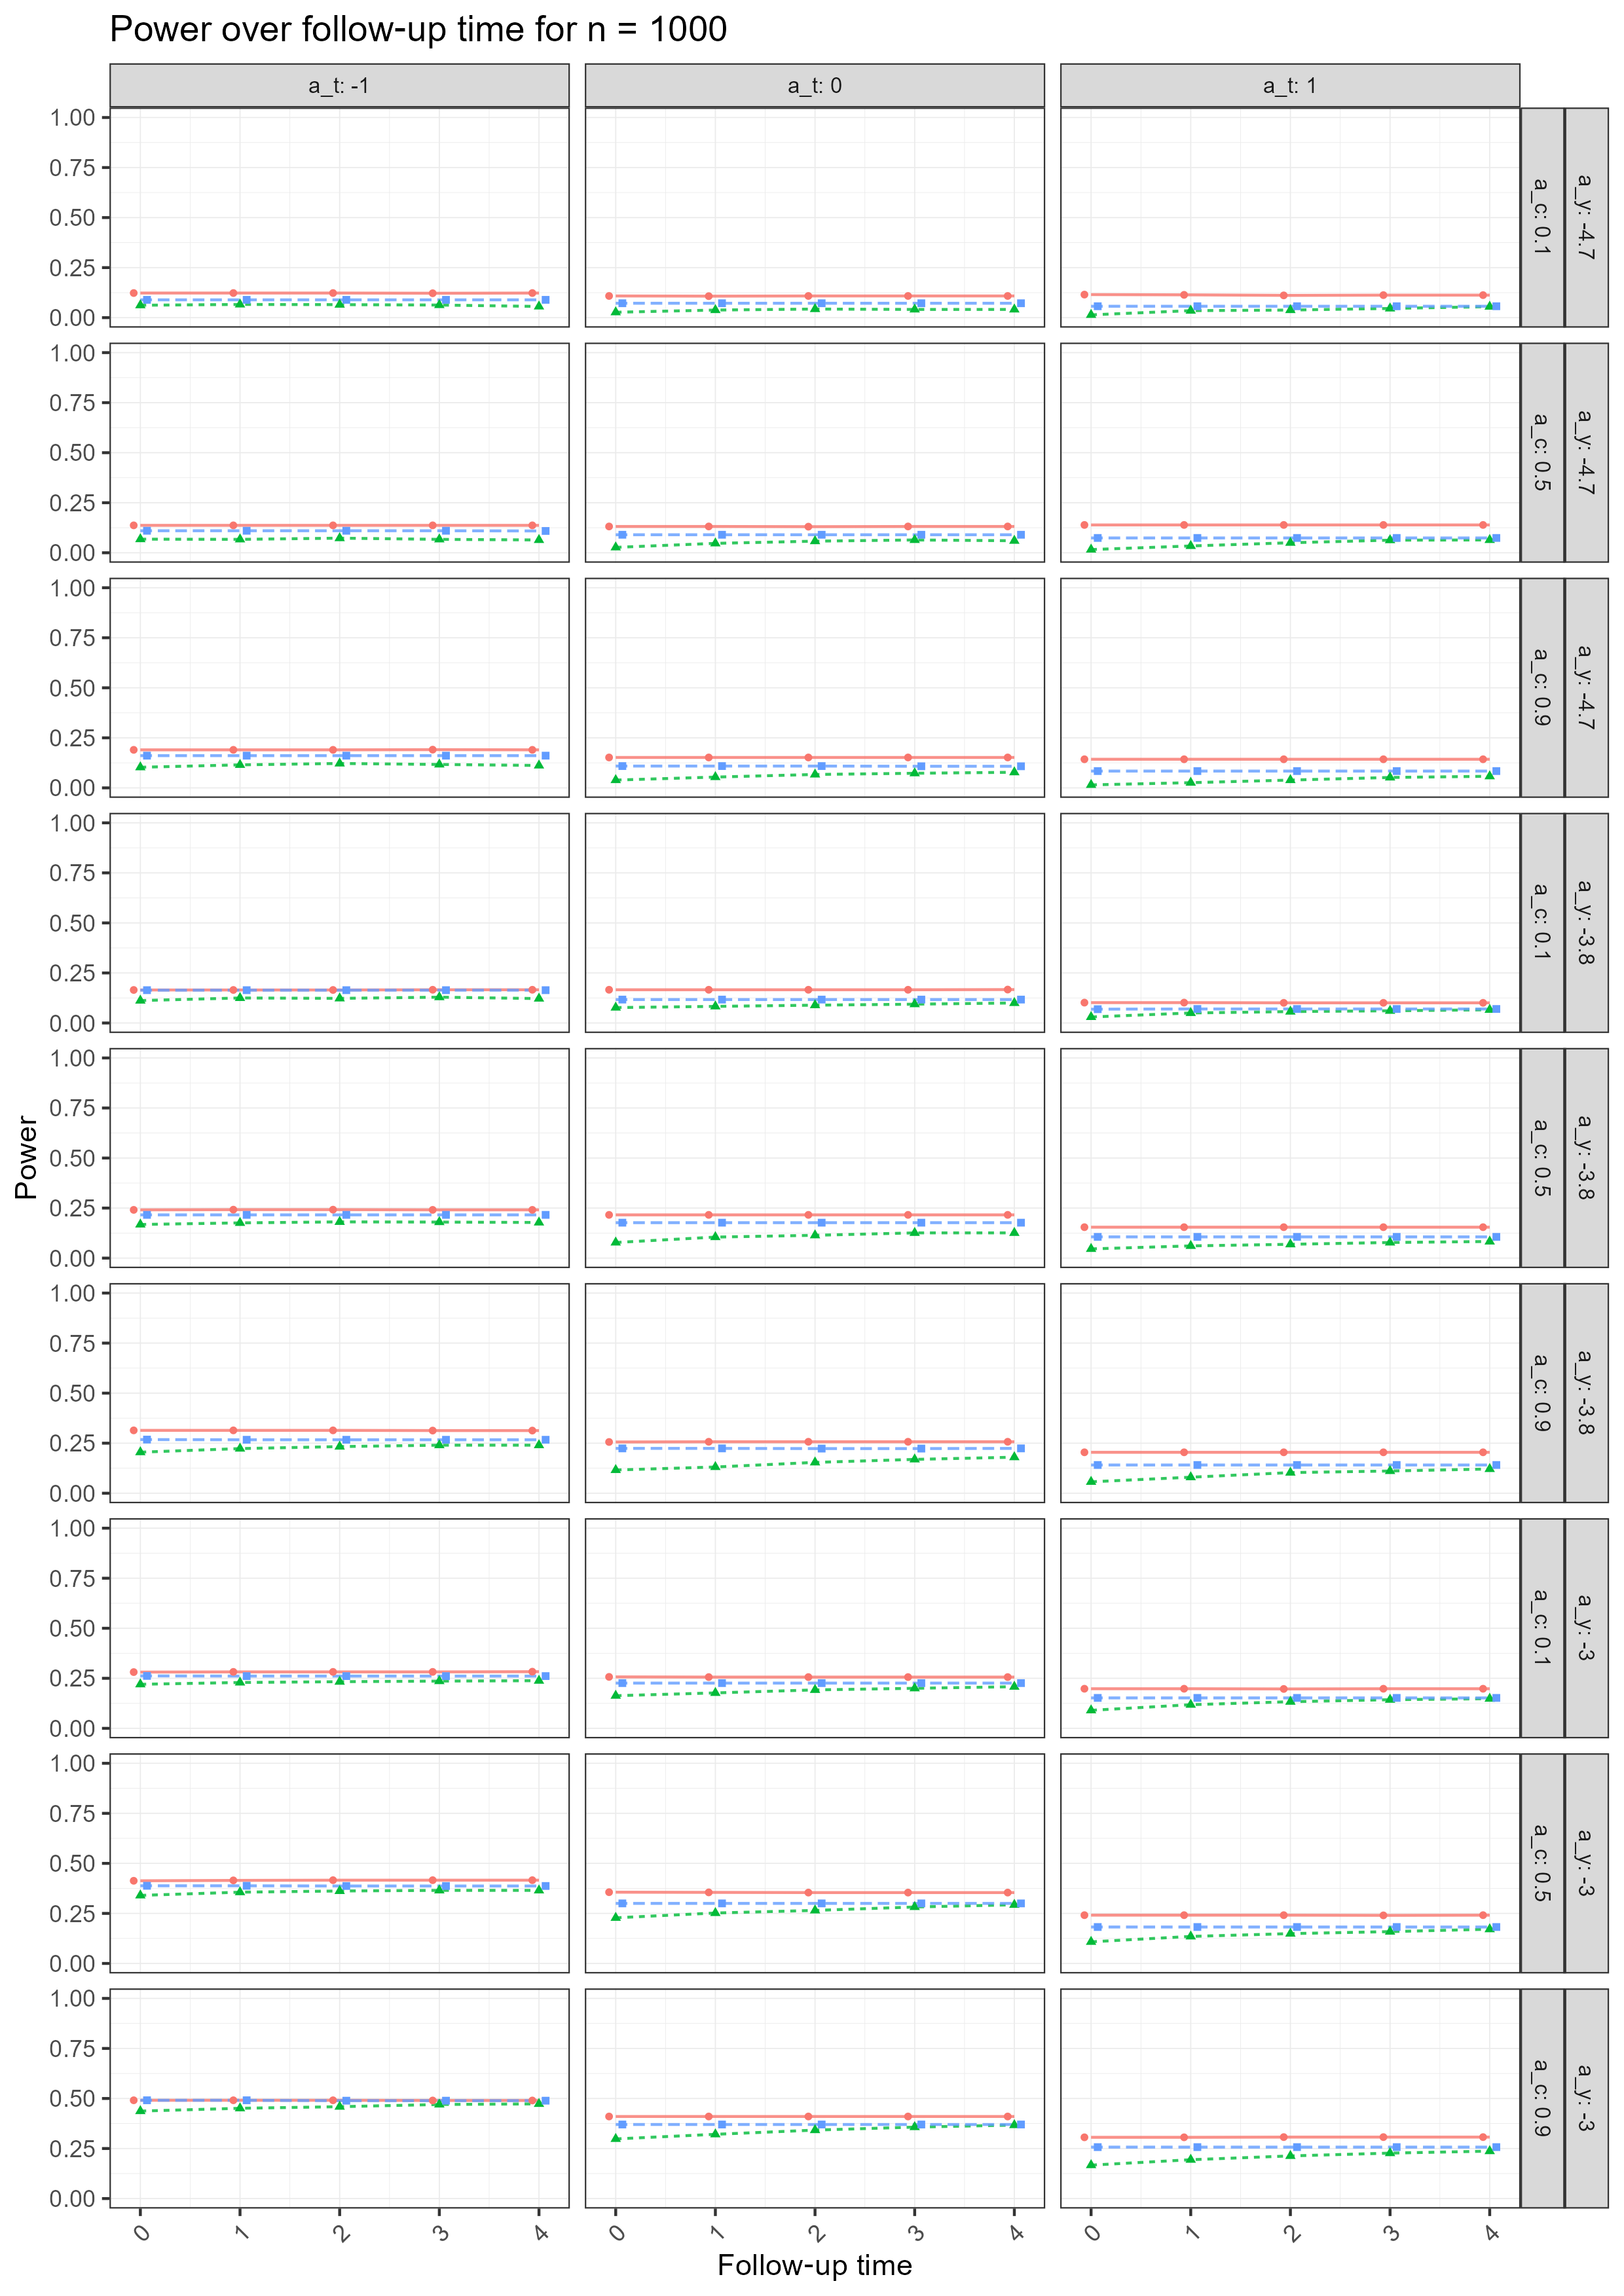
\includegraphics[height=0.95\textheight]{plots/plots_power1000.png}
\caption{Power of the $95\%$ confidence interval over $1000$ simulations with sample size $n = 1000$. The green line denotes \textcolor{green}{the empirical bootstrap CI}, the blue line denotes \textcolor{blue}{percentile bootstrap CI}, and the red line denotes \textcolor{red}{sandwich estimator CI}. The outcome event rate indicator is denoted by $a_y$, the confounding strength is denoted by $a_c$, and the treatment prevalence indicator is denoted by $a_t$.}
\label{plt:power1000}
\end{figure}

\newpage

\begin{figure}[H]
\centering
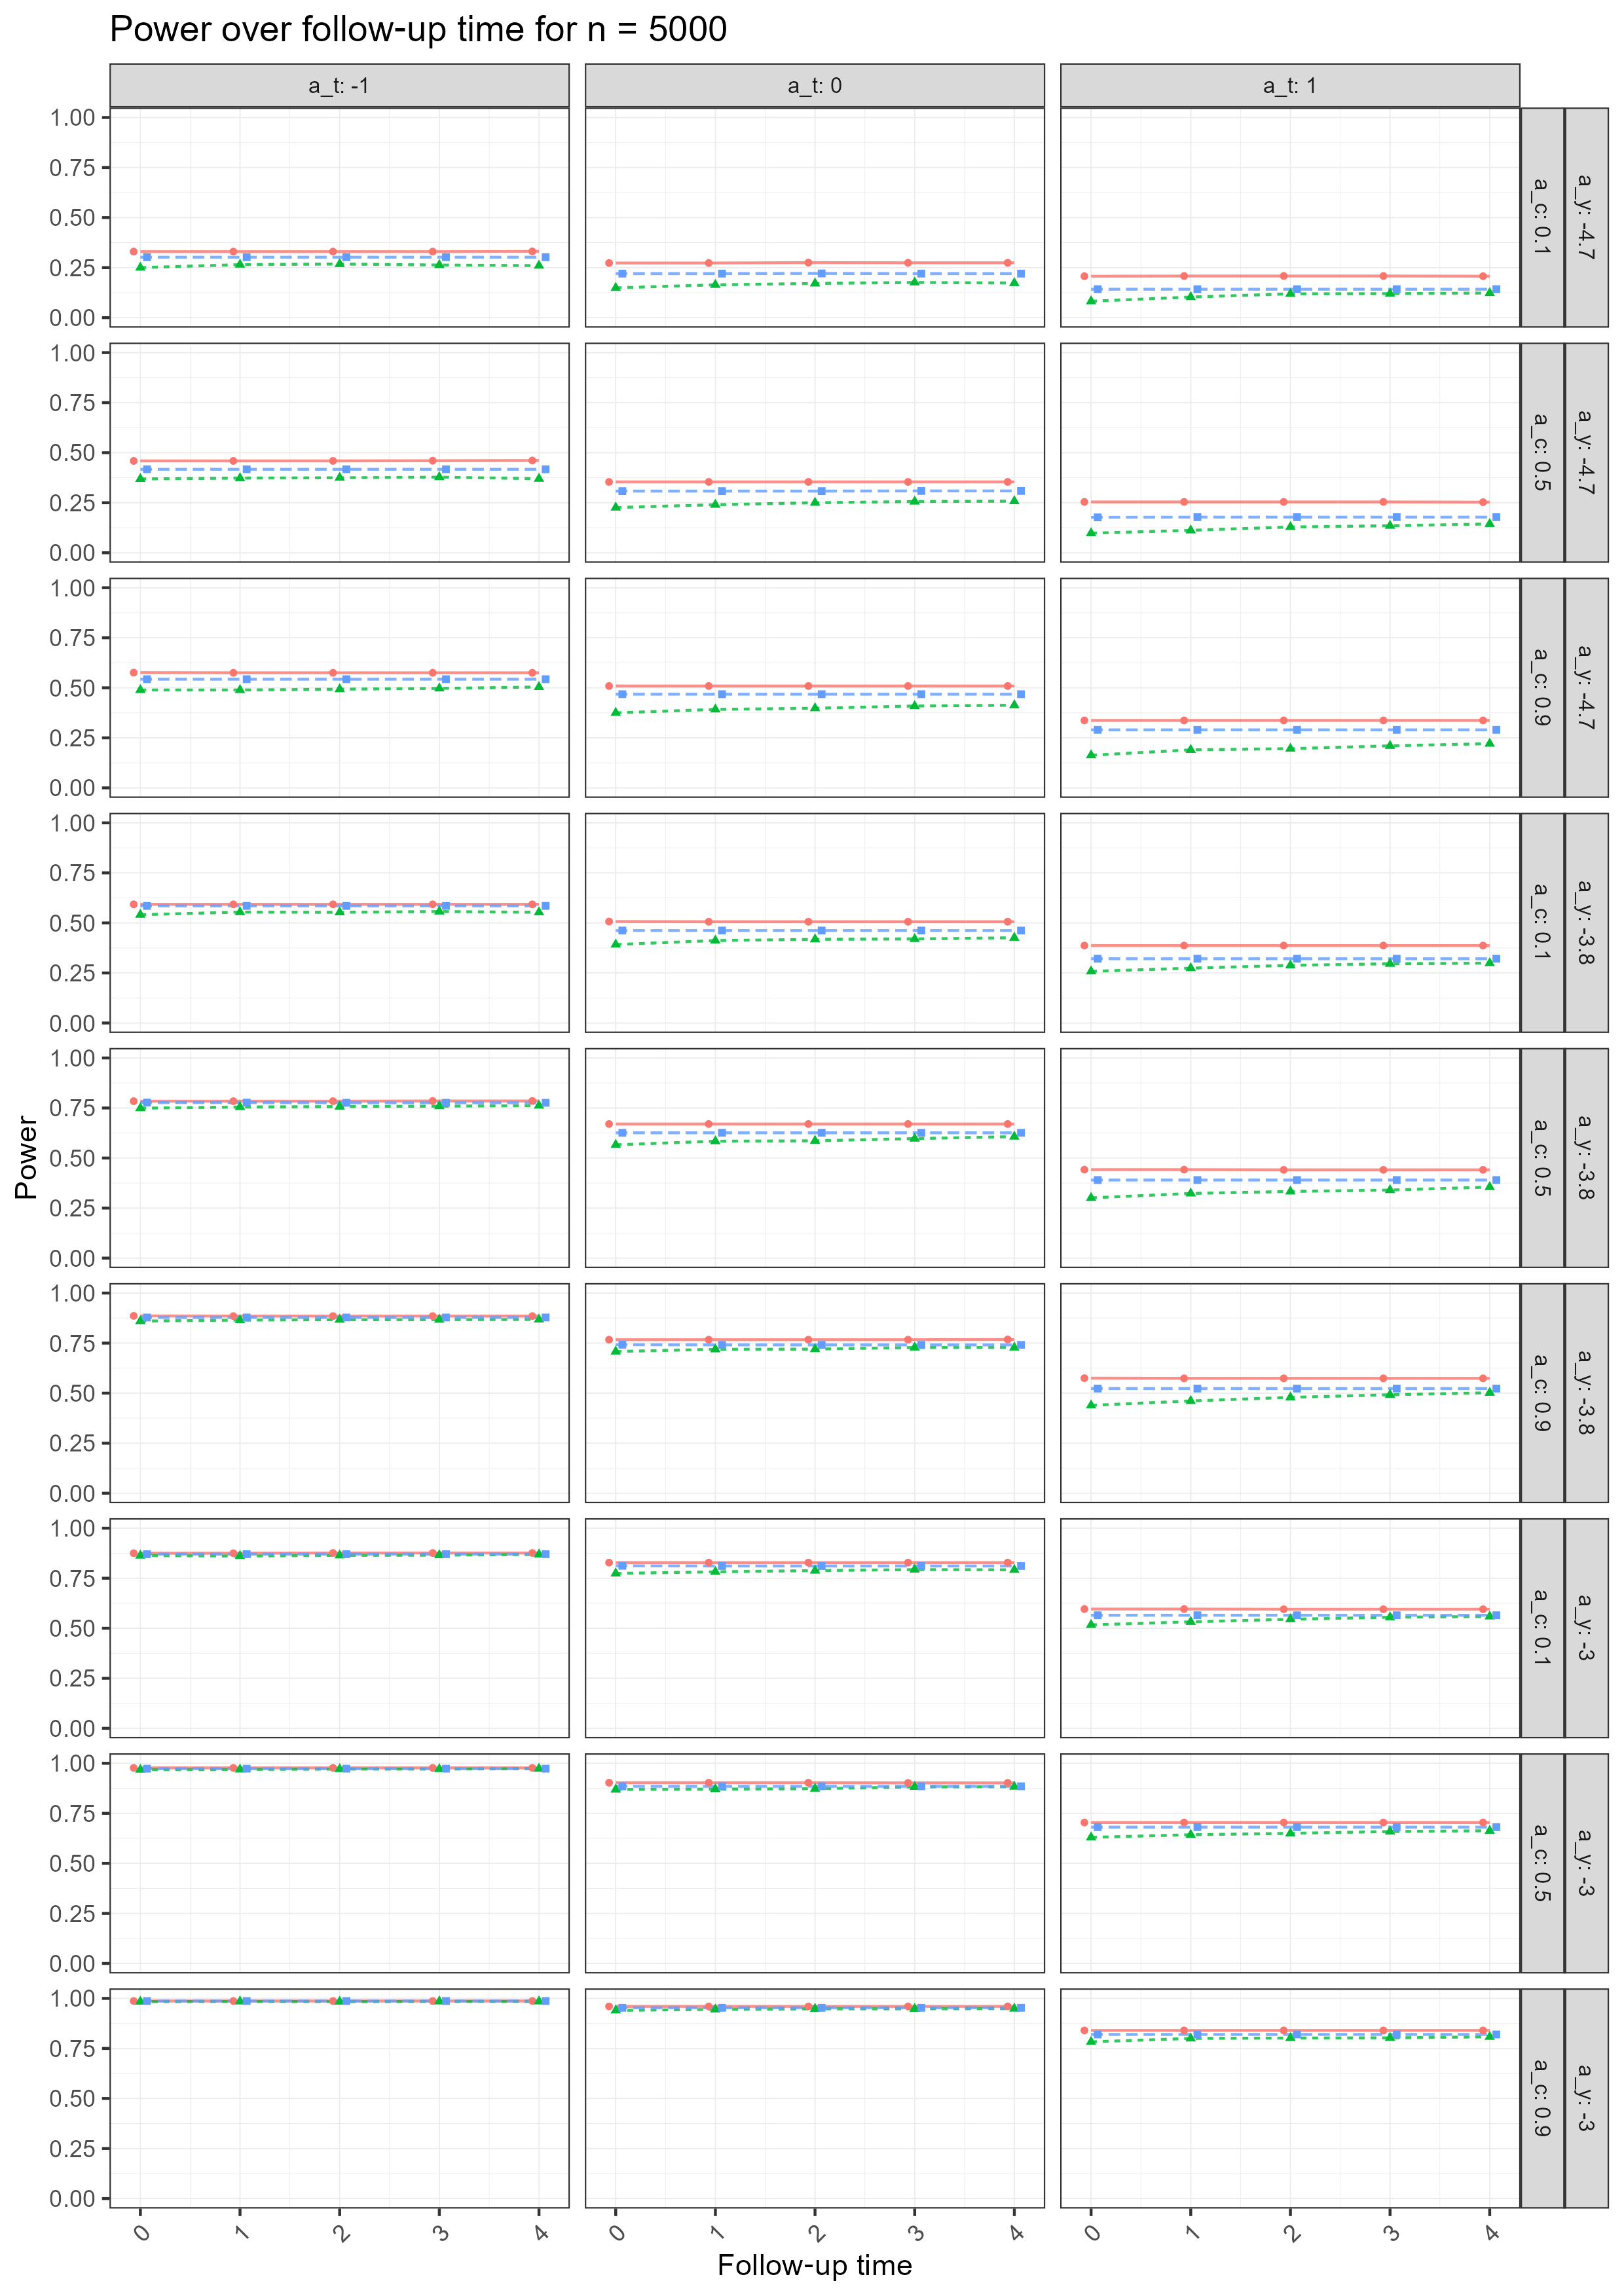
\includegraphics[height=0.95\textheight]{plots/plots_power5000.png}
\caption{Power of the $95\%$ confidence interval over $1000$ simulations with sample size $n = 5000$. The green line denotes \textcolor{green}{the empirical bootstrap CI}, the blue line denotes \textcolor{blue}{percentile bootstrap CI}, and the red line denotes \textcolor{red}{sandwich estimator CI}. The outcome event rate indicator is denoted by $a_y$, the confounding strength is denoted by $a_c$, and the treatment prevalence indicator is denoted by $a_t$.}
\label{plt:power5000}
\end{figure}

\newpage


\section{Results Simulation: Point Estimates}\label{ApxSim1PE}

In Appendix~\ref{ApxSim1PE} we present all plots regarding the point estimates. The specific numbers to each plot can be found in the online supplementary materials on \url{https://github.com/flo1met/thesis_TTE}.

\newpage

\begin{figure}[H]
\centering
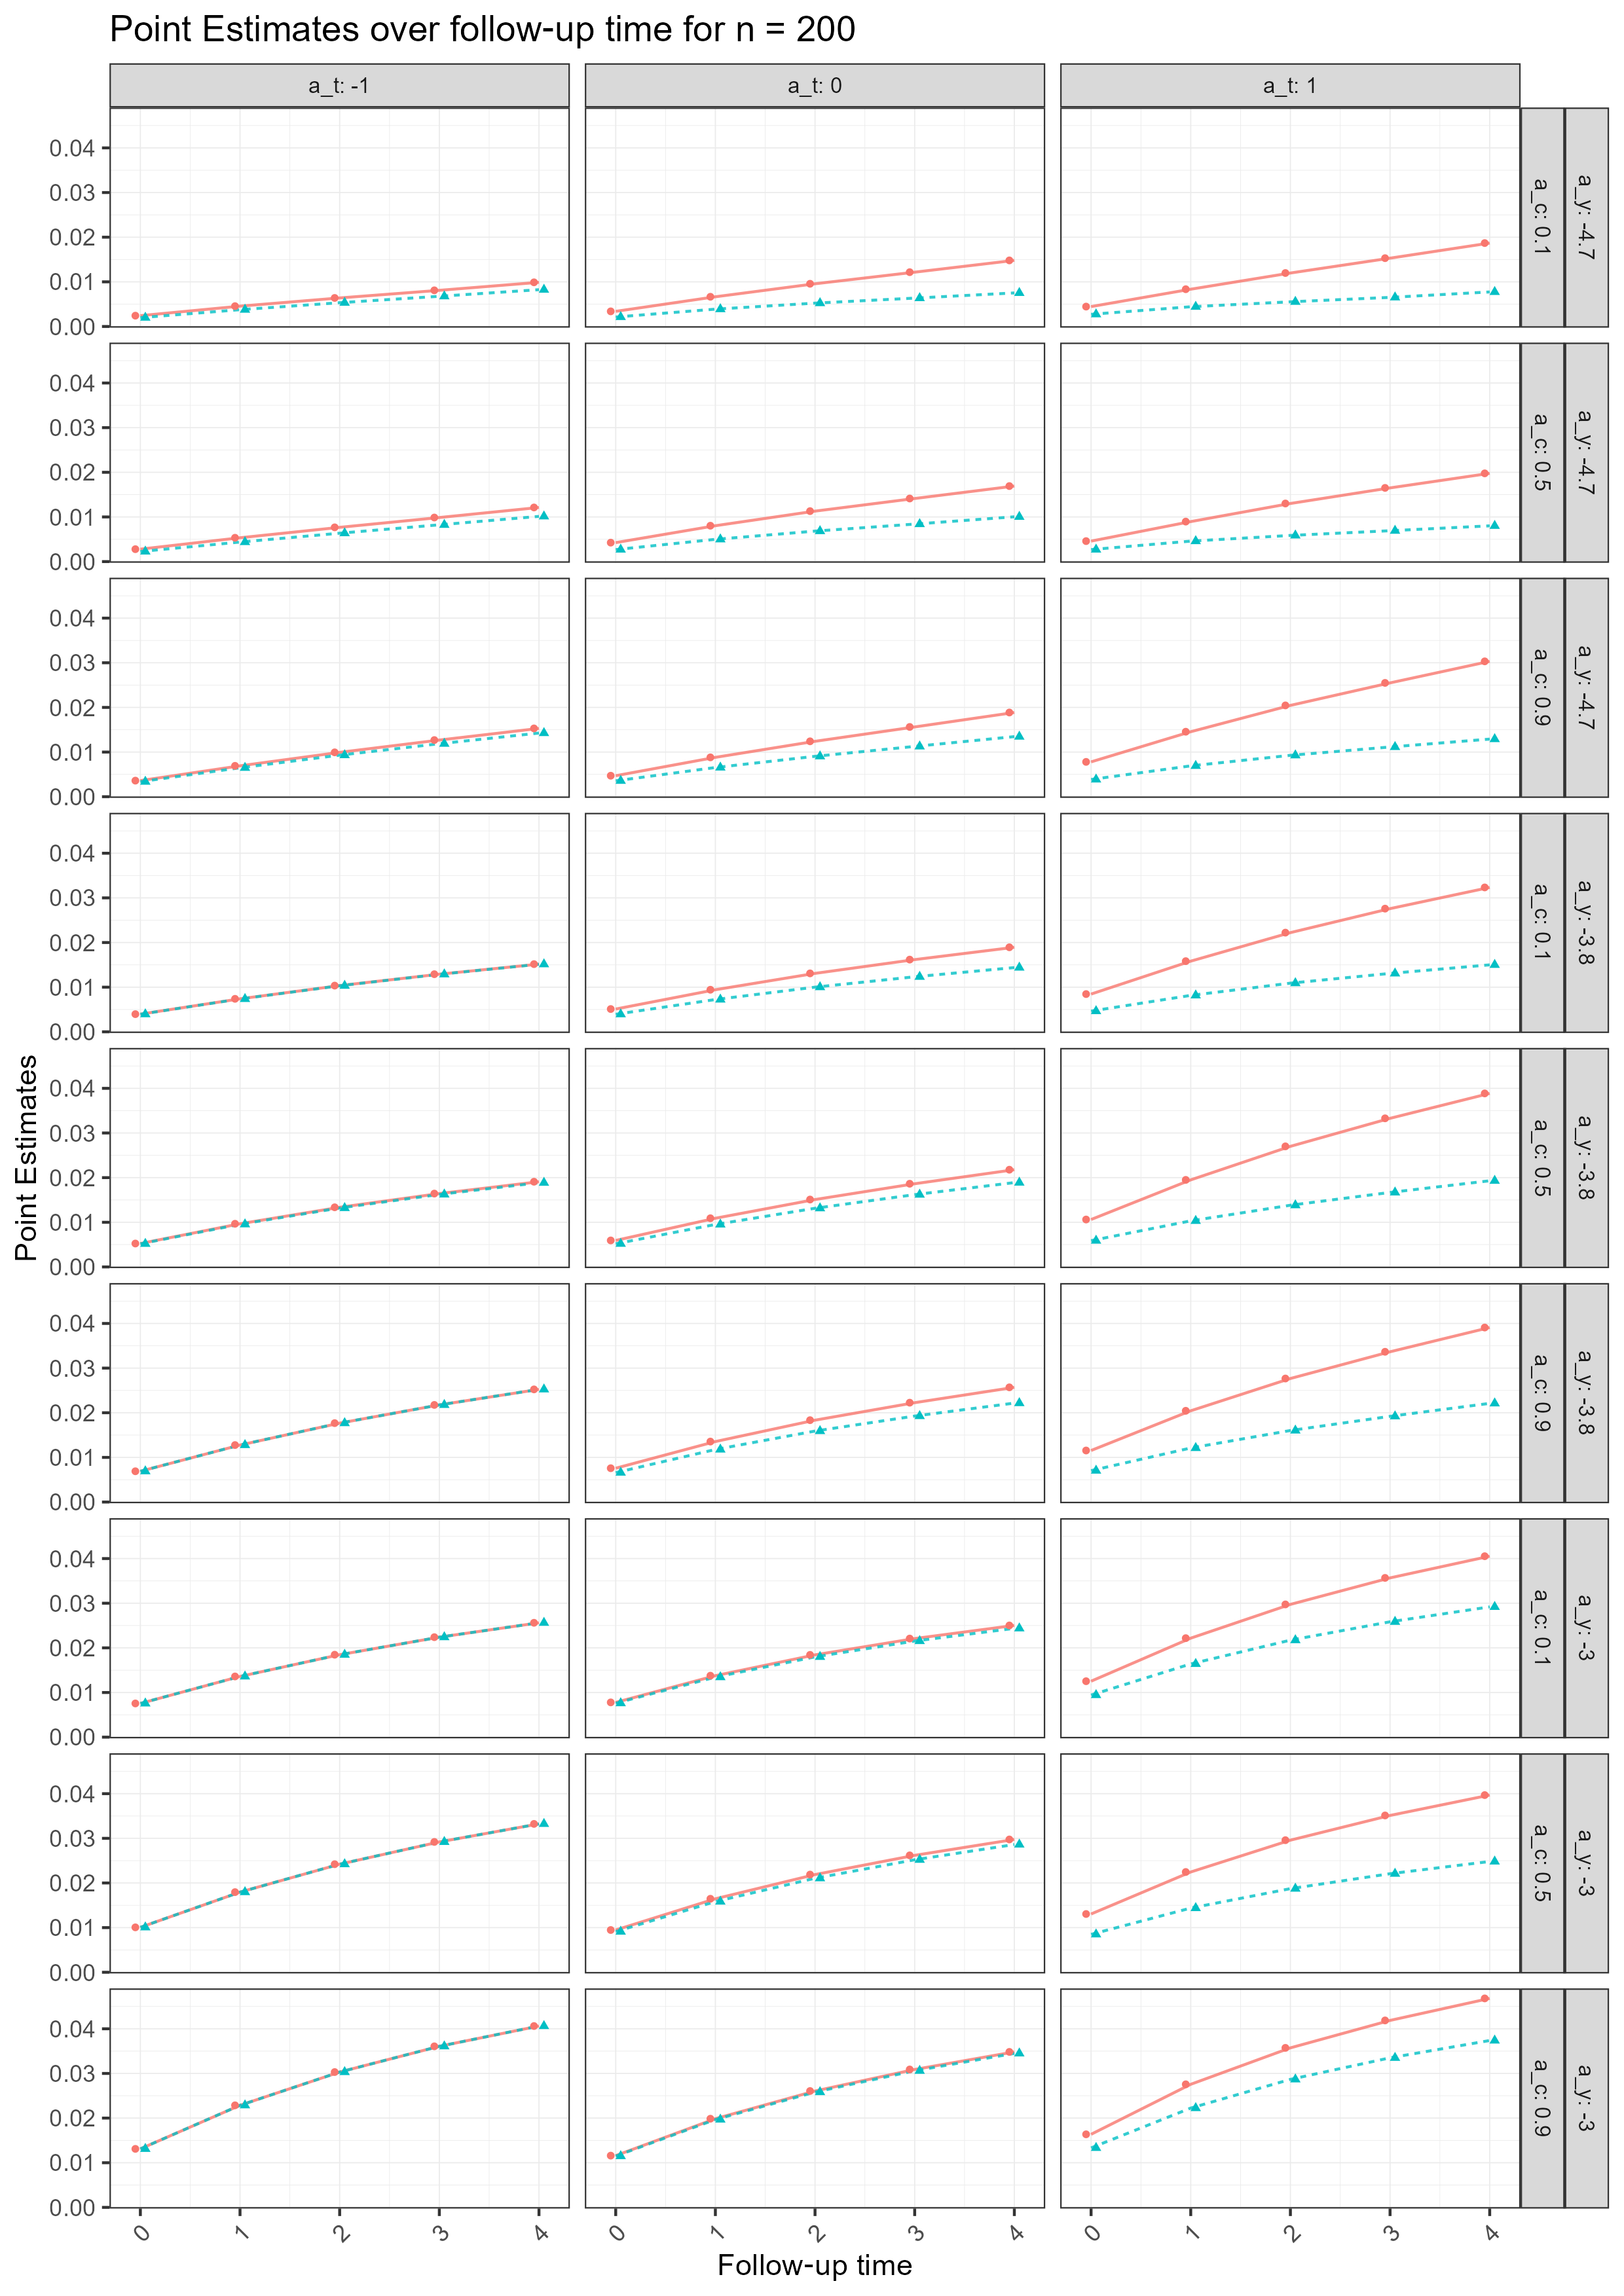
\includegraphics[height=0.95\textheight]{plots/plots_PE200.png}
\caption{Comparison of $\widehat{\operatorname{MRD}}$ point estimates between \textcolor{red}{\Rlang{}} and \textcolor{green}{\julia{}} over $1000$ simulations with sample size $n = 200$. The red line shows the \textcolor{red}{\Rlang{} point estimates}, and the blue line shows the \textcolor{blue}{\julia{} point estimates}. The outcome event rate indicator is denoted by $a_y$, the confounding strength is denoted by $a_c$, and the treatment prevalence indicator is denoted by $a_t$.}
\label{plt:PE200}
\end{figure}

\newpage

\begin{figure}[H]
\centering
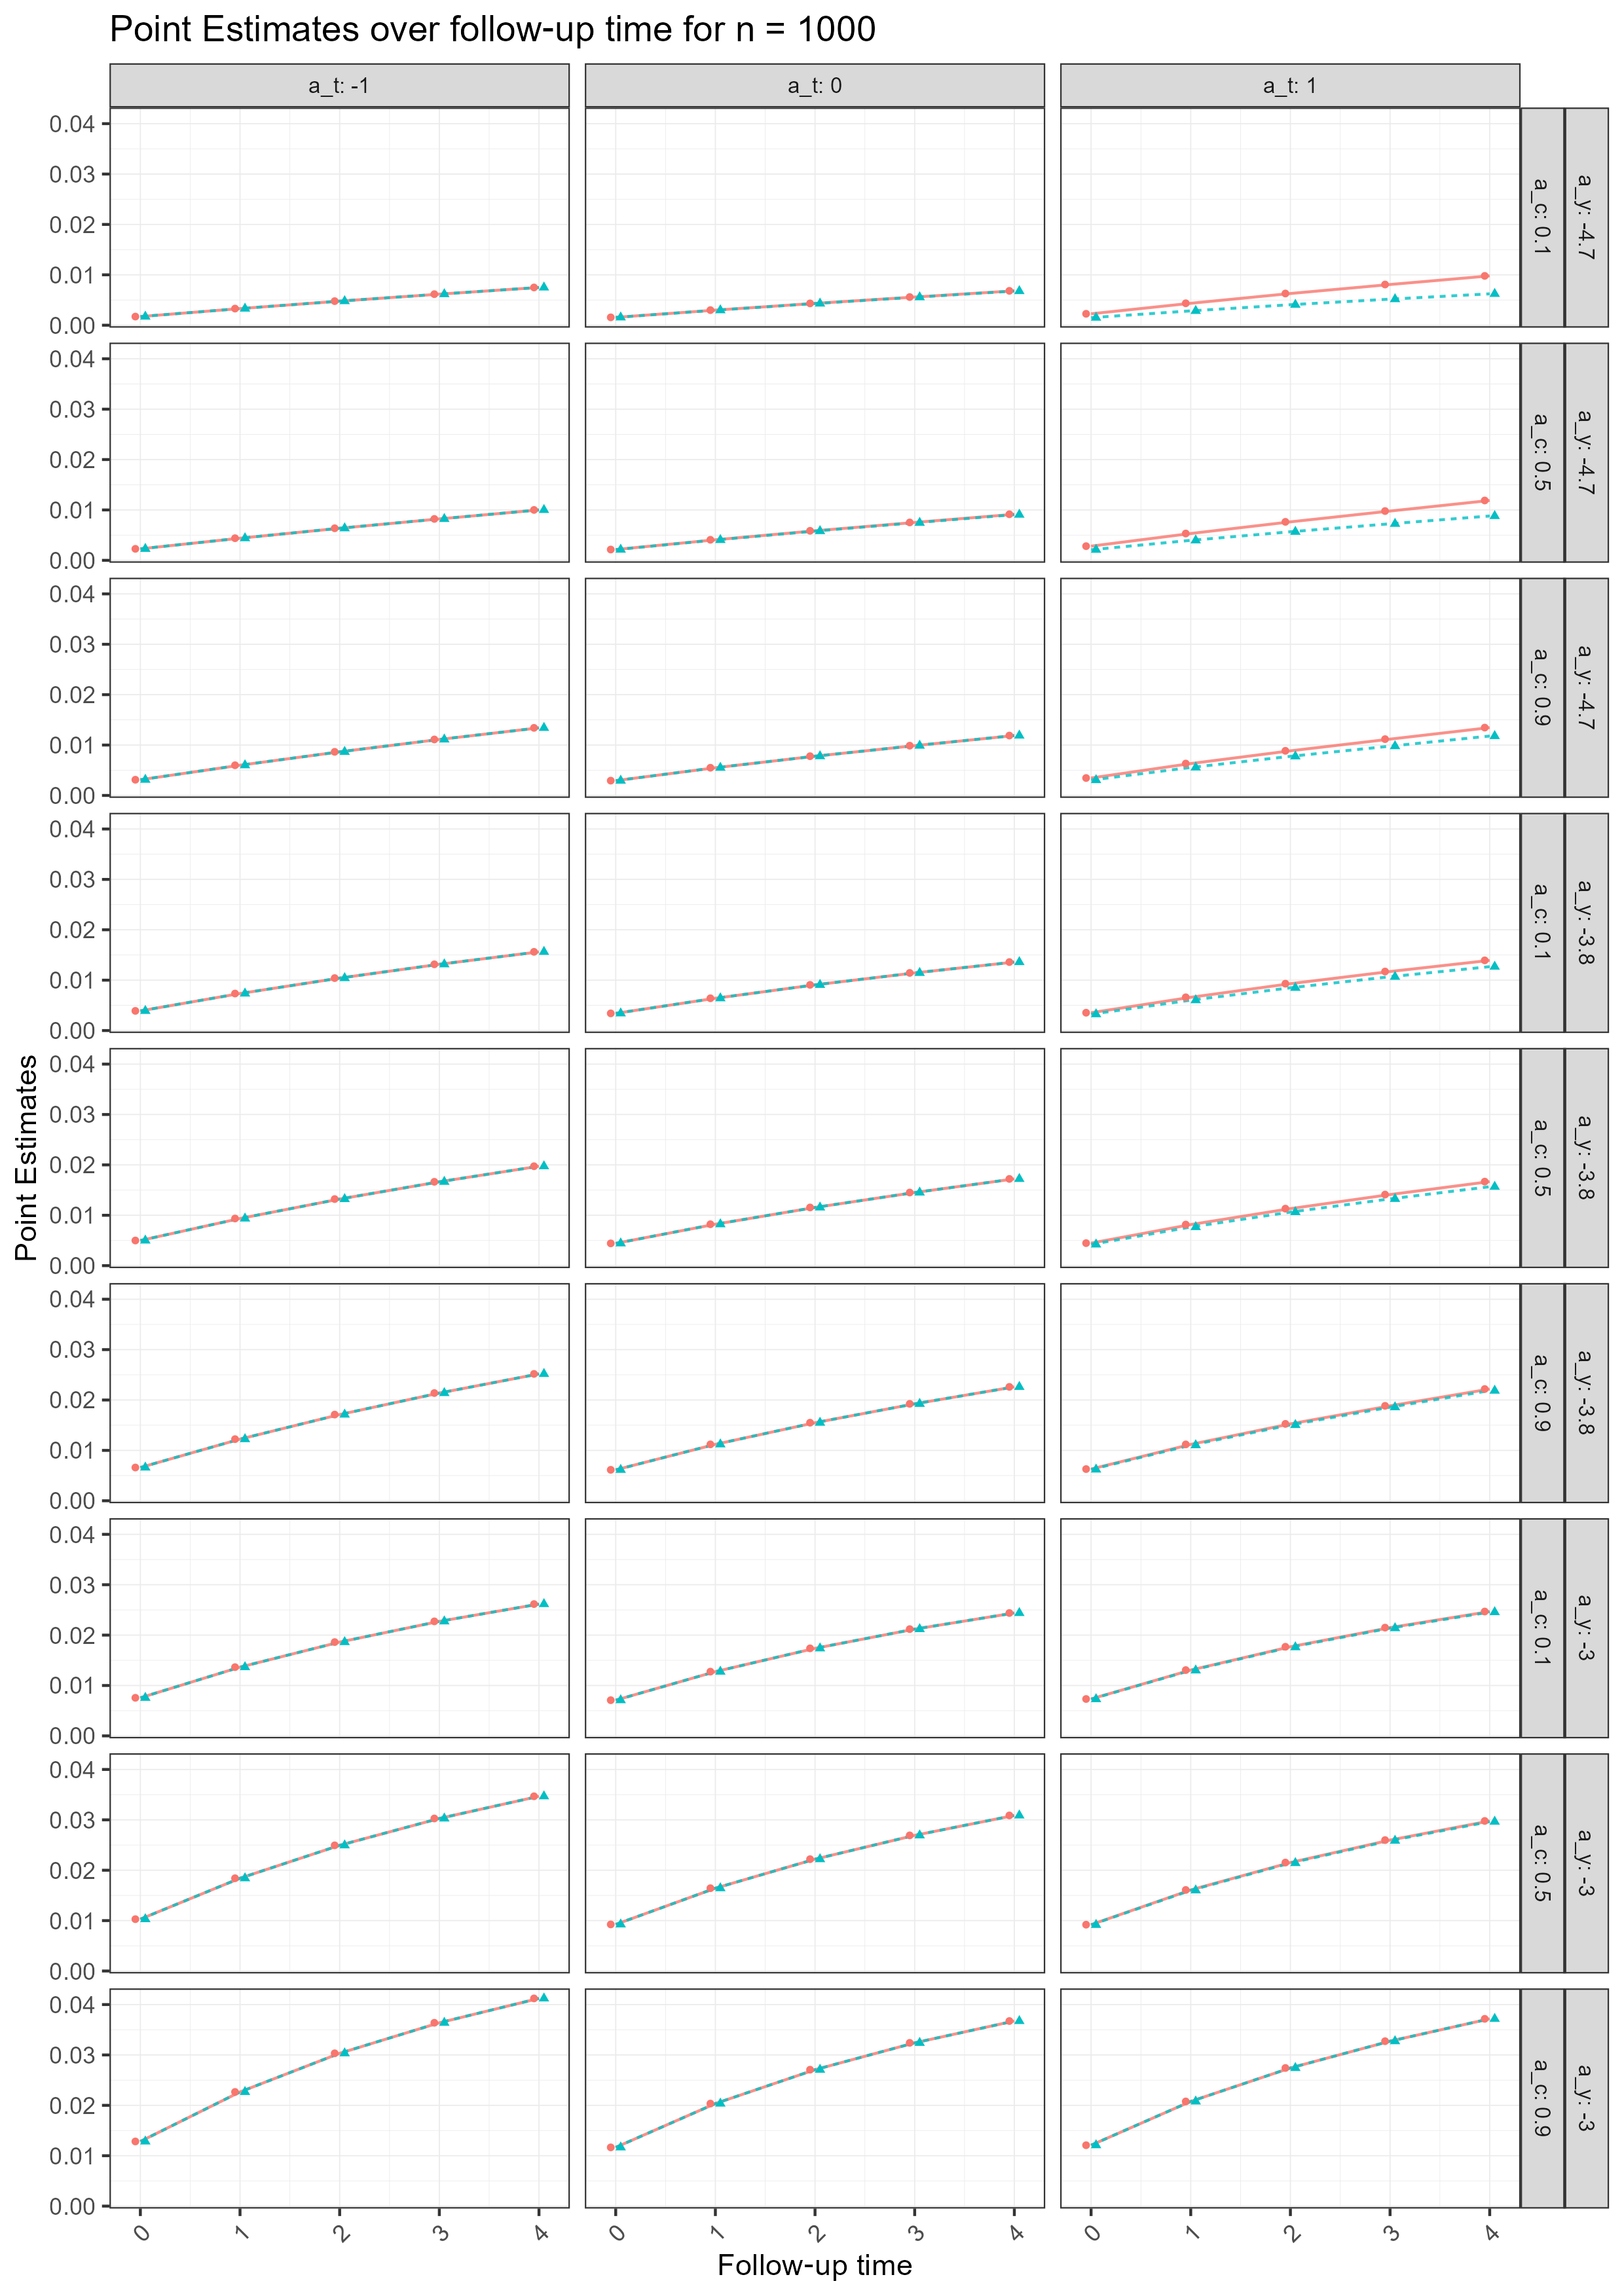
\includegraphics[height=0.95\textheight]{plots/plots_PE1000.png}
\caption{Comparison of $\widehat{\operatorname{MRD}}$ point estimates between \textcolor{red}{\Rlang{}} and \textcolor{green}{\julia{}} over $1000$ simulations with sample size $n = 1000$. The red line shows the \textcolor{red}{\Rlang{} point estimates}, and the blue line shows the \textcolor{blue}{\julia{} point estimates}. The outcome event rate indicator is denoted by $a_y$, the confounding strength is denoted by $a_c$, and the treatment prevalence indicator is denoted by $a_t$.}
\label{plt:PE1000}
\end{figure}

\newpage

\begin{figure}[H]
\centering
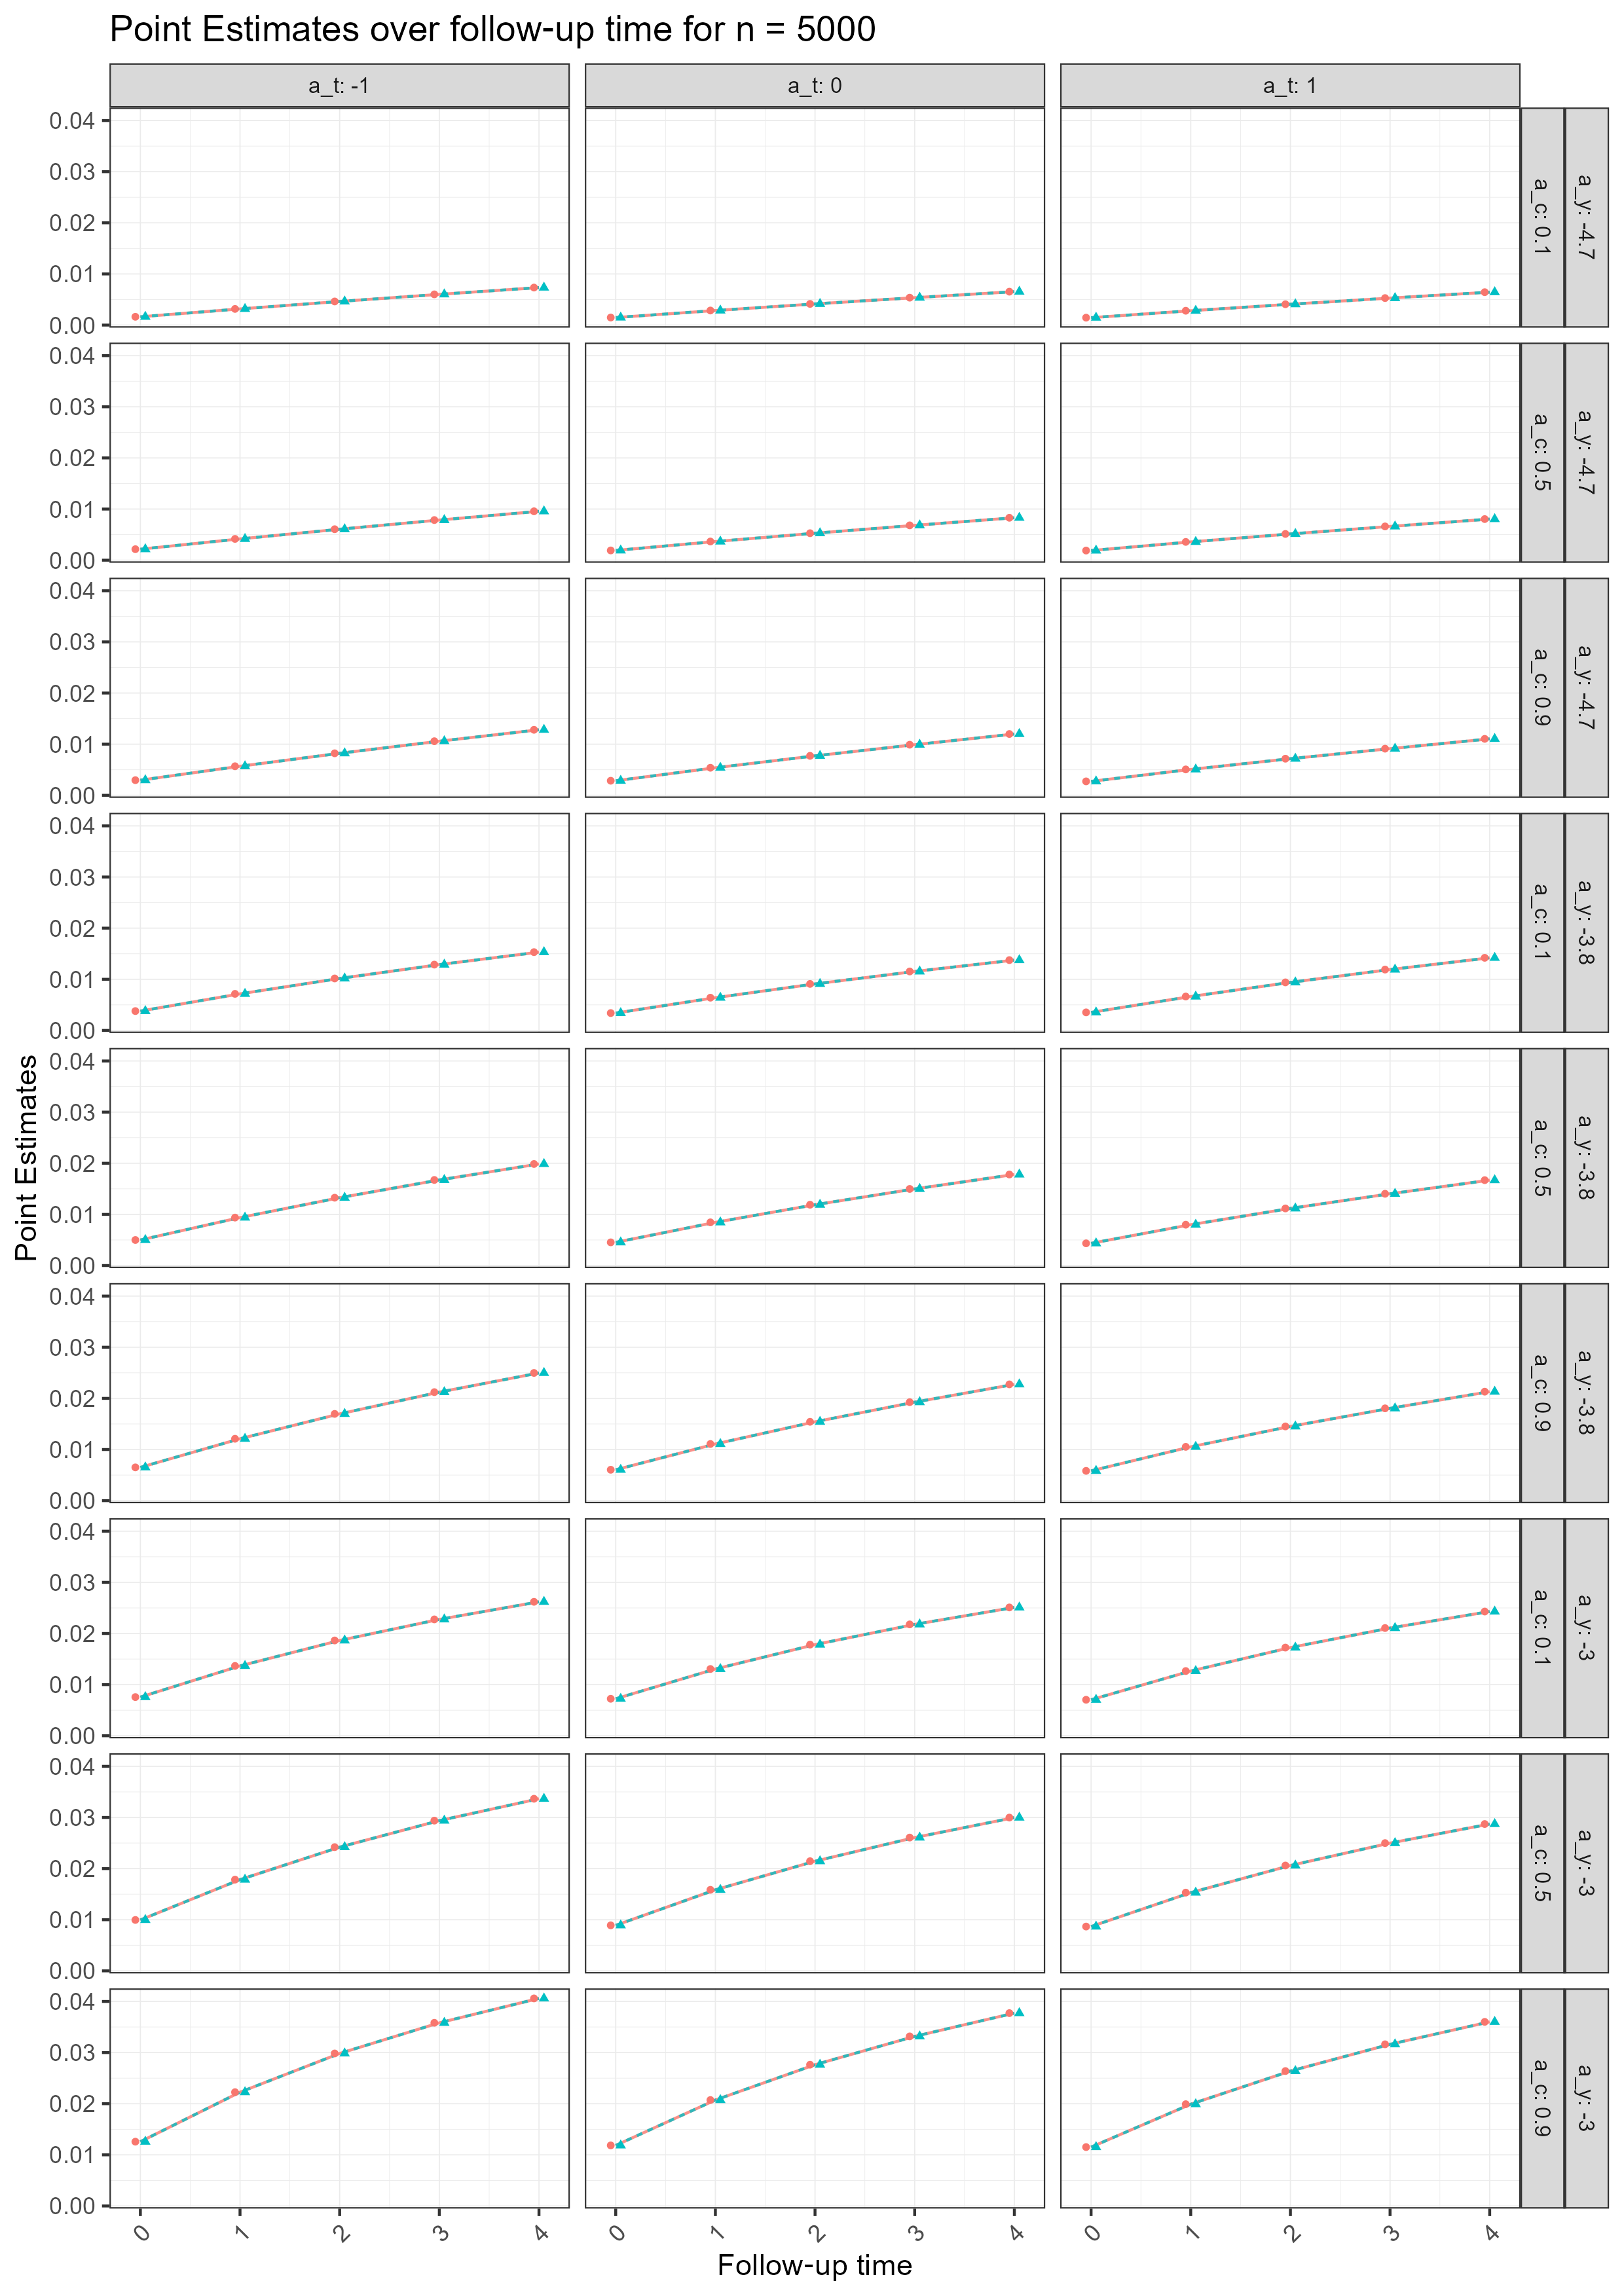
\includegraphics[height=0.95\textheight]{plots/plots_PE5000.png}
\caption{Comparison of $\widehat{\operatorname{MRD}}$ point estimates between \textcolor{red}{\Rlang{}} and \textcolor{green}{\julia{}} over $1000$ simulations with sample size $n = 5000$. The red line shows the \textcolor{red}{\Rlang{} point estimates}, and the blue line shows the \textcolor{blue}{\julia{} point estimates}. The outcome event rate indicator is denoted by $a_y$, the confounding strength is denoted by $a_c$, and the treatment prevalence indicator is denoted by $a_t$.}
\label{plt:PE5000}
\end{figure}

\newpage

\begin{figure}[H]
\centering
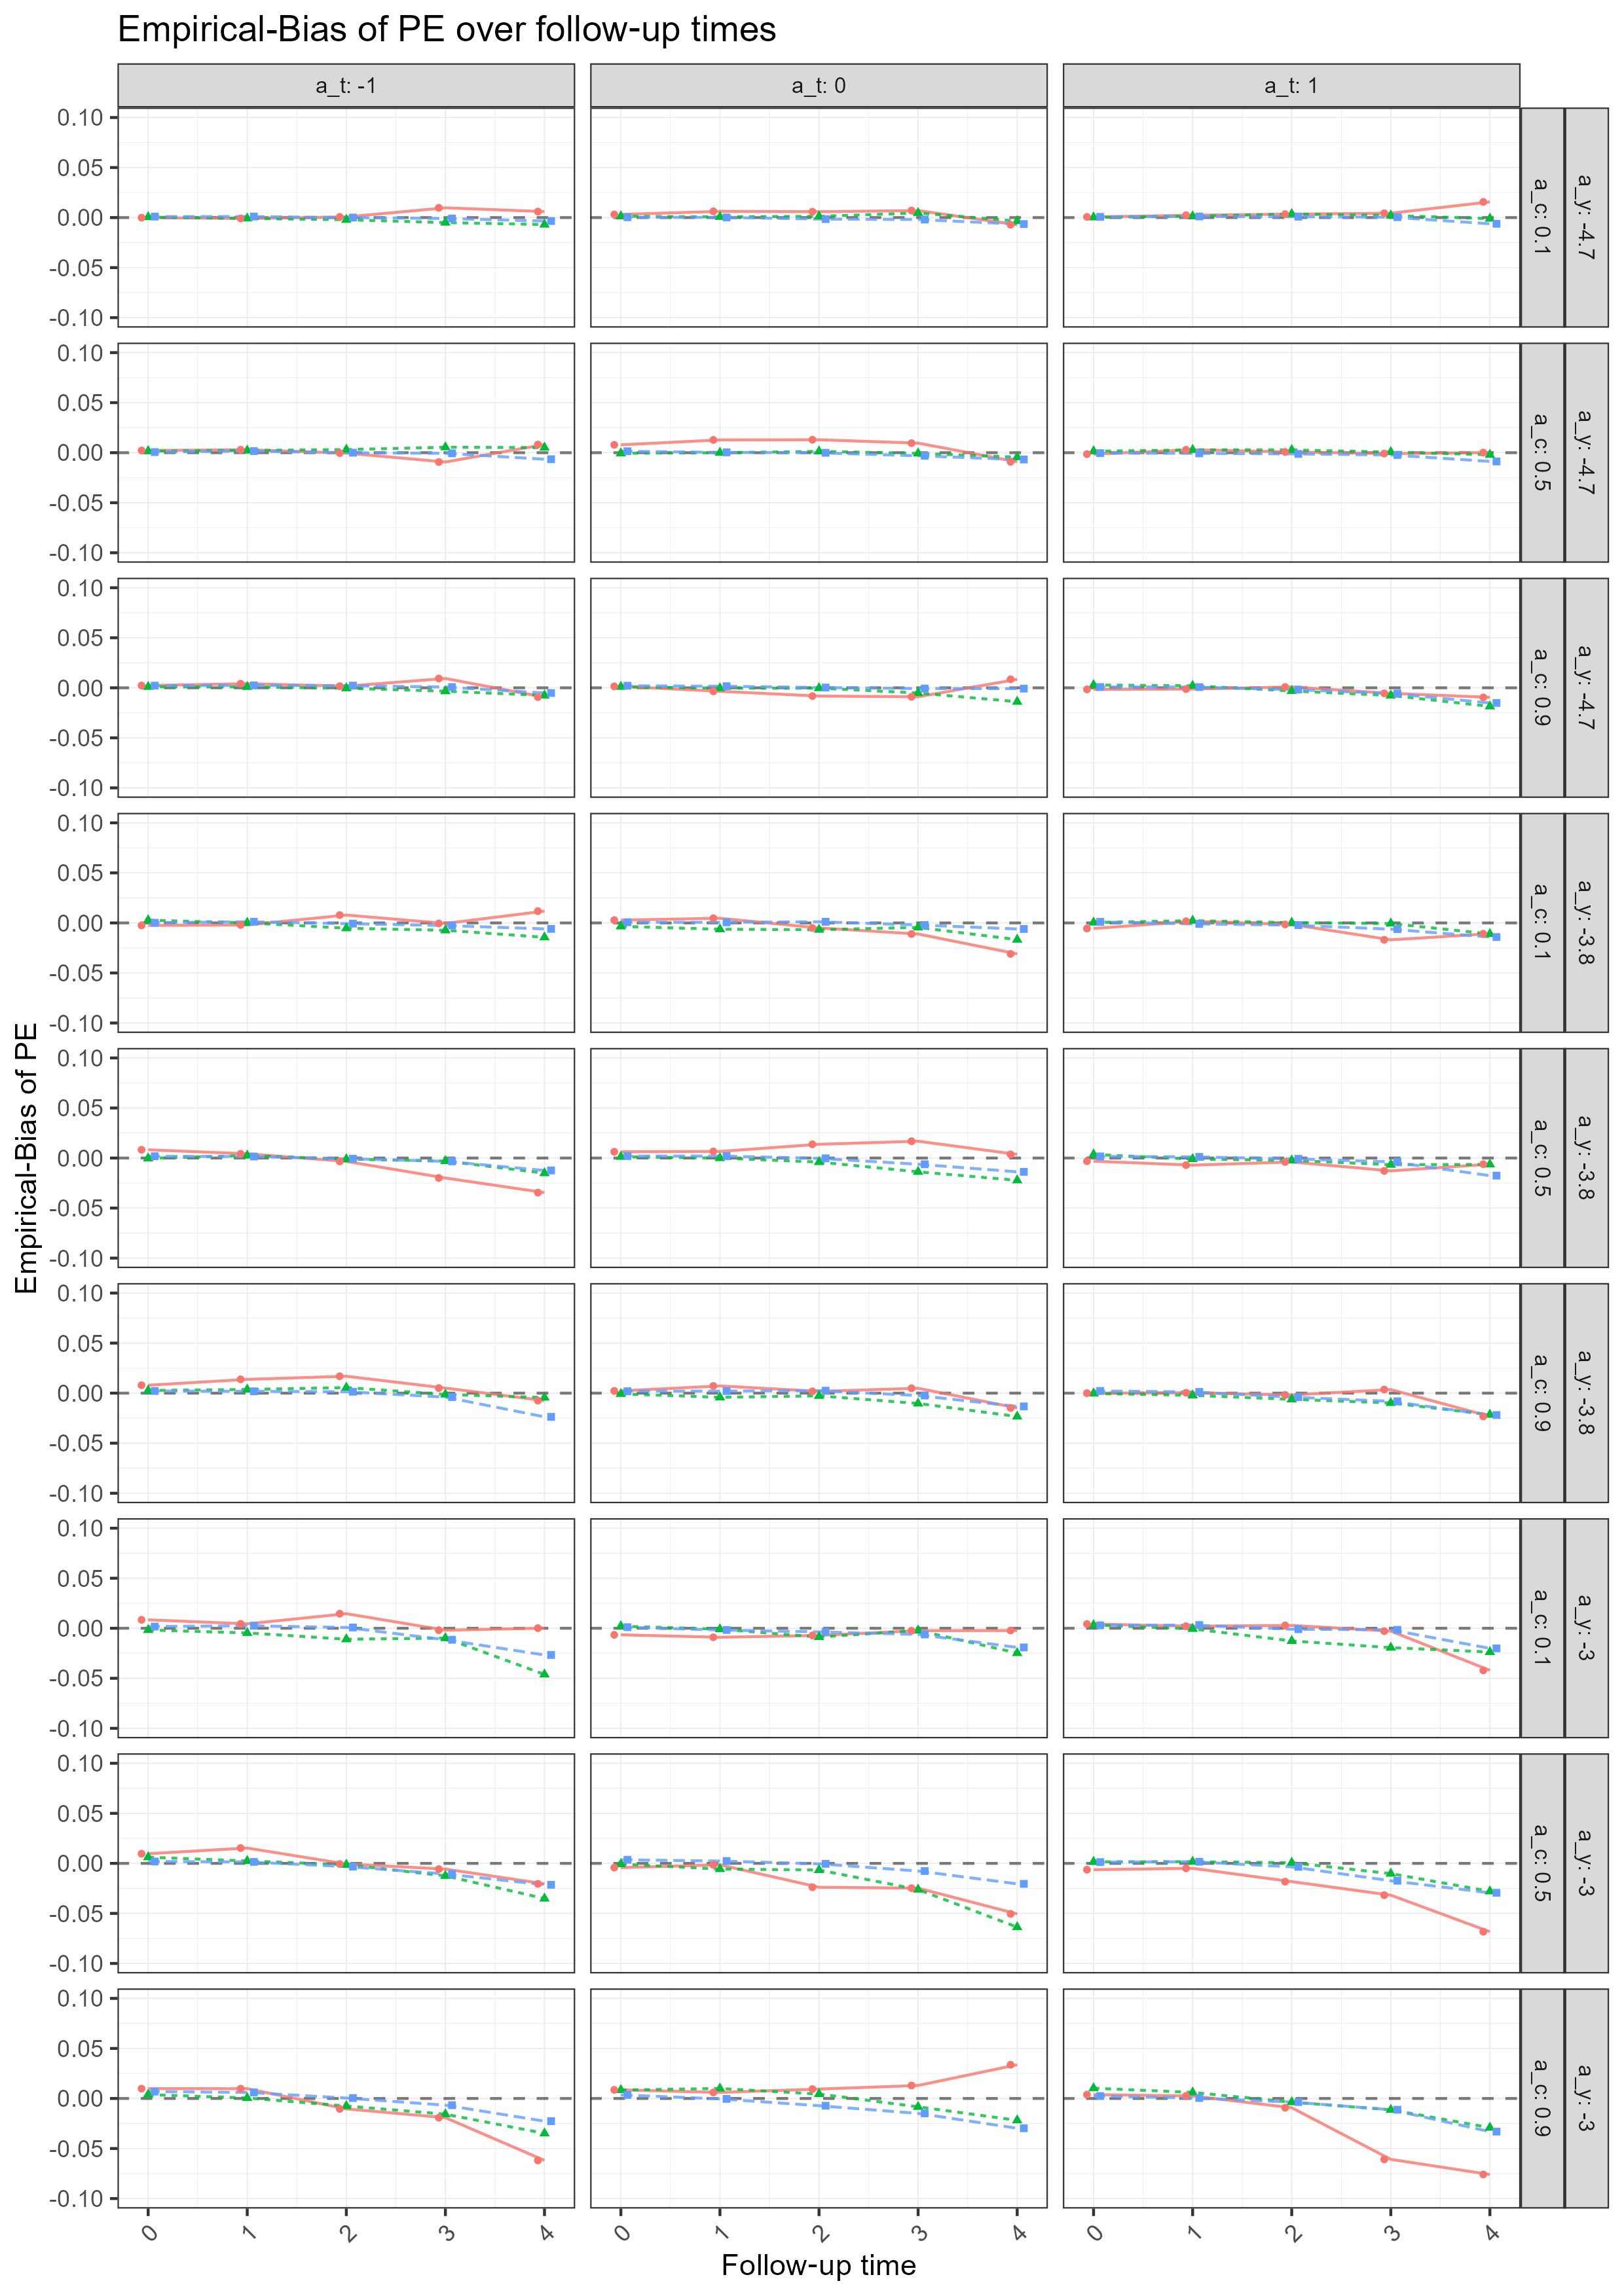
\includegraphics[height=0.95\textheight]{plots/plots_PE_bias.png}
\caption{Bias of the $\widehat{\operatorname{MRD}}$ point estimates over $1000$ simulations. The red line denotes the \textcolor{red}{sample size $n = 200$}, the green line denotes the \textcolor{green}{sample size $n = 1000$}, and the blue line denotes the \textcolor{blue}{sample size $n = 5000$}. The dashed gray line marks the reference value \textcolor{darkgray}{$0$}. The outcome event rate indicator is denoted by $a_y$, the confounding strength is denoted by $a_c$, and the treatment prevalence indicator is denoted by $a_t$.}\label{plt:bias}
\end{figure}

\newpage

\begin{figure}[H]
\centering
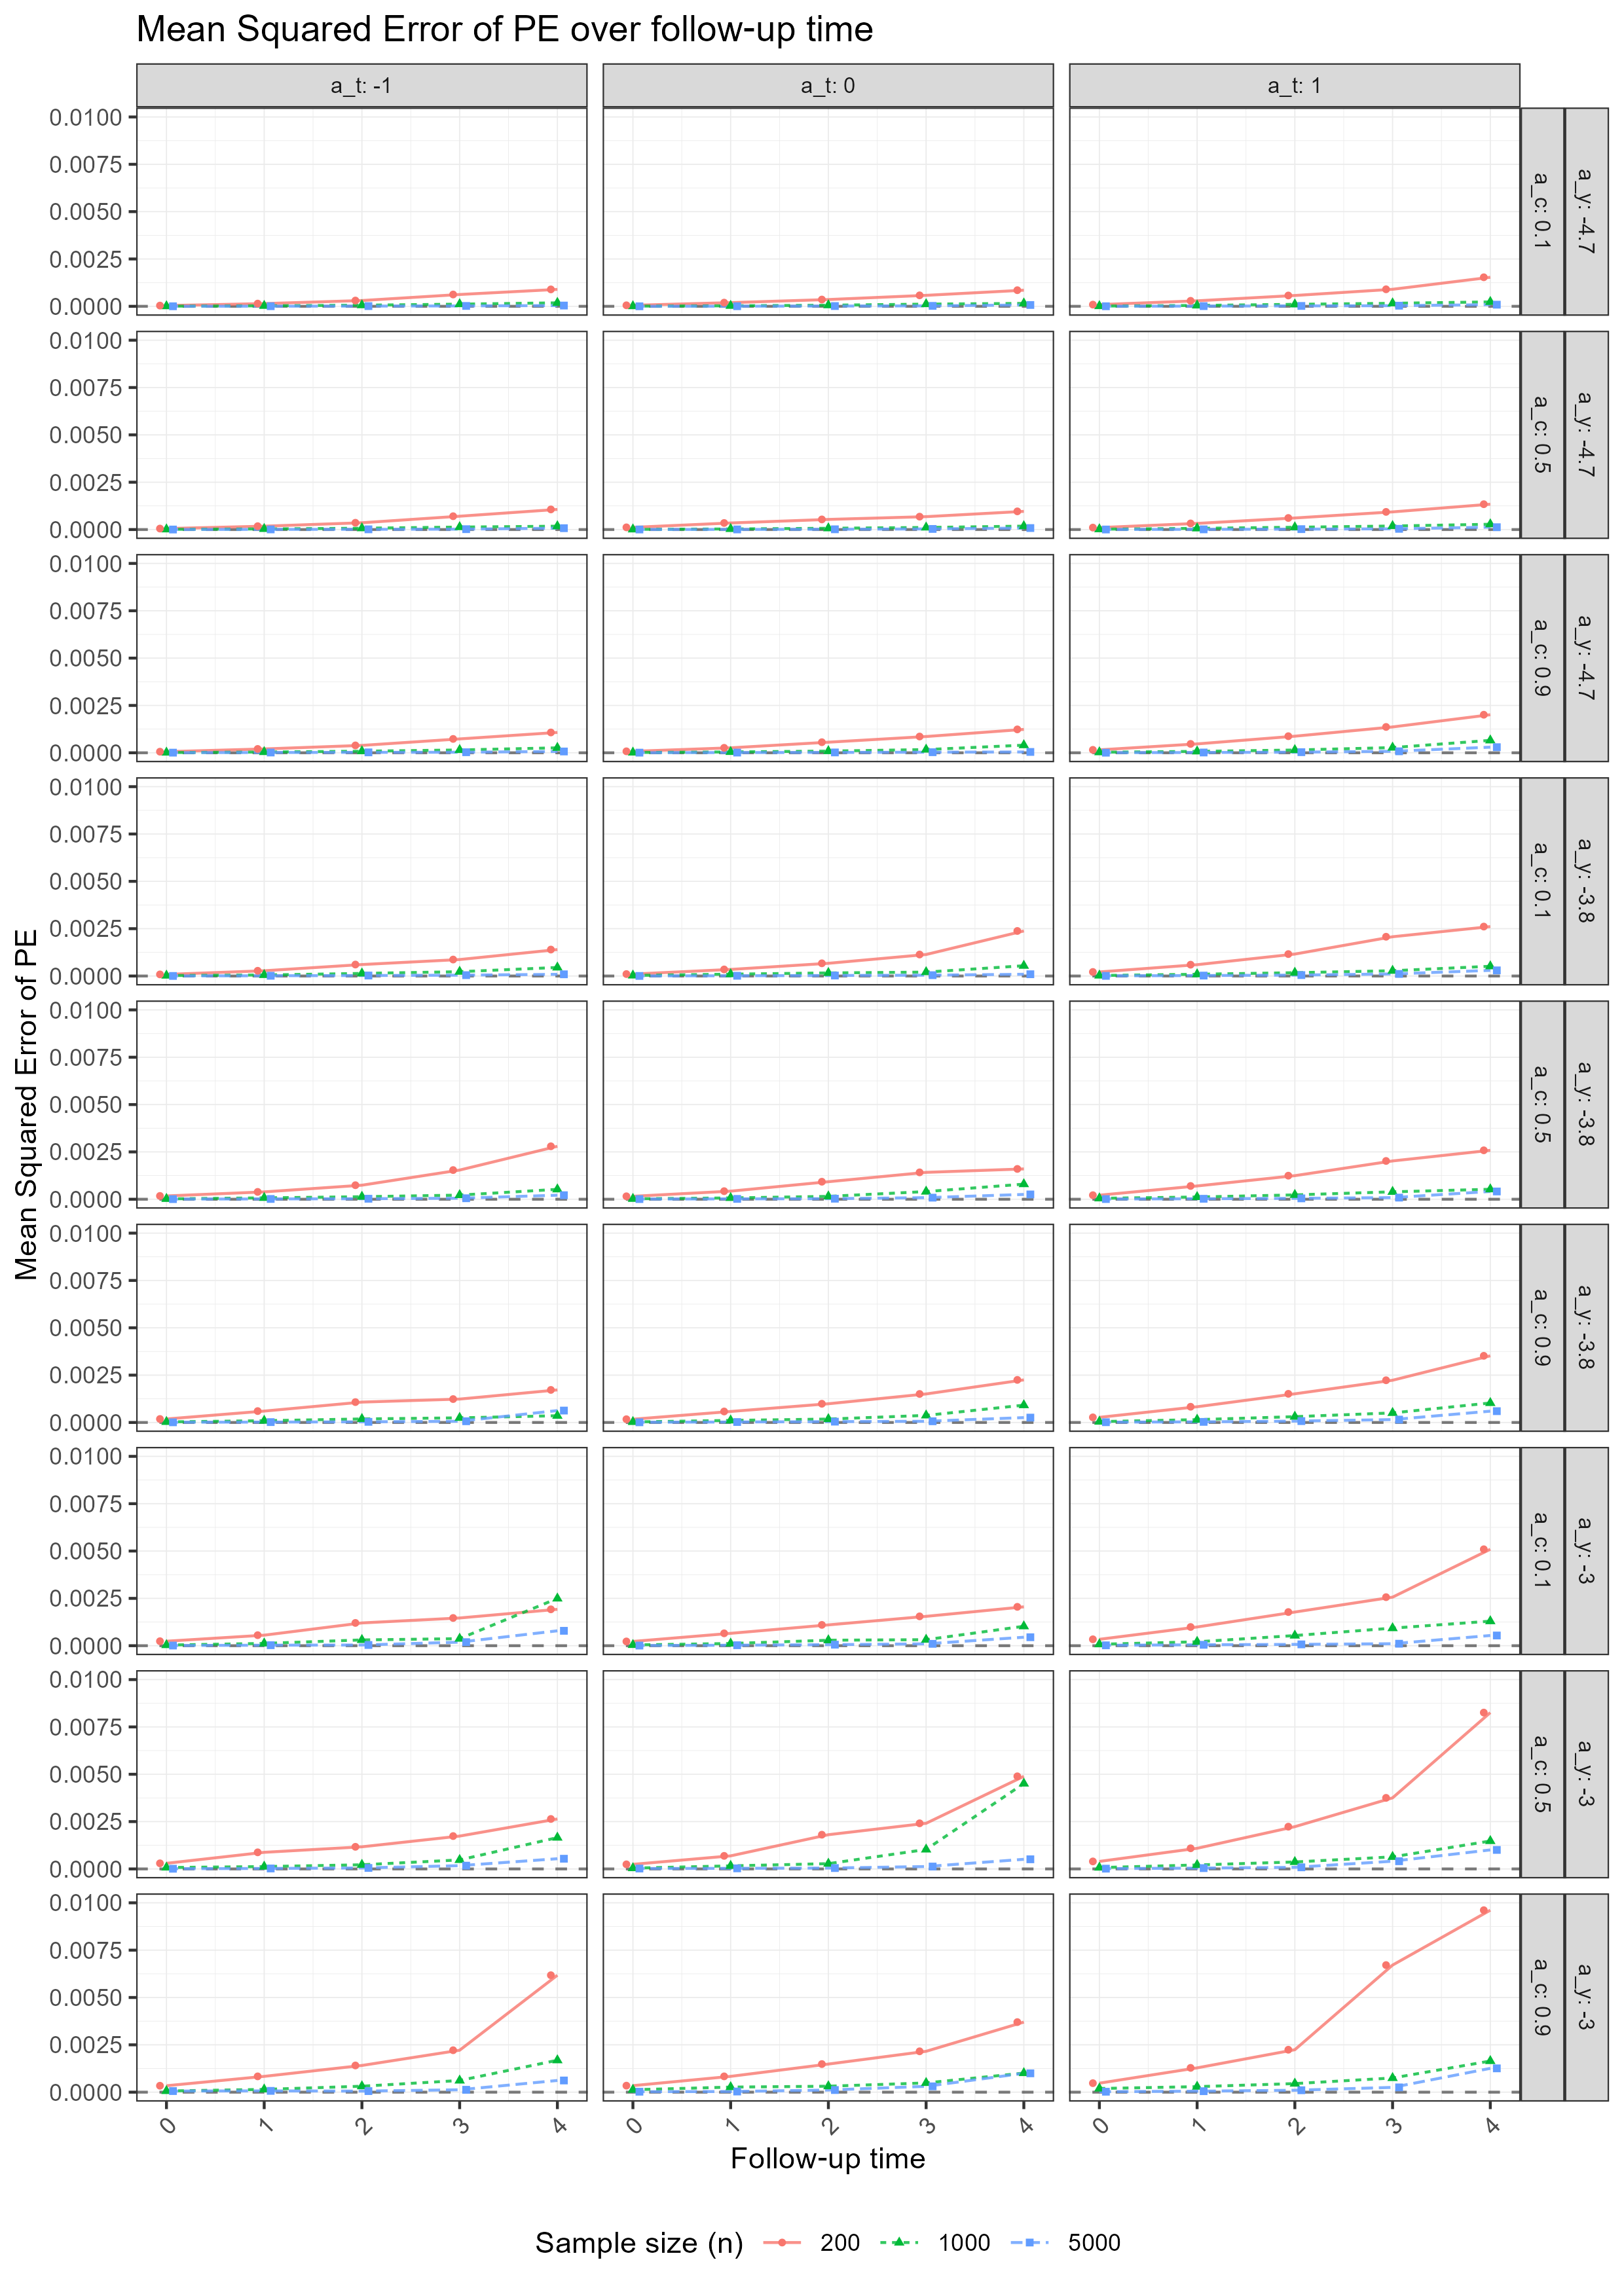
\includegraphics[height=0.95\textheight]{plots/plots_PE_MSE.png}
\caption{Mean Squared Error (MSE) of the $\widehat{\operatorname{MRD}}$ point estimates over $1000$ simulations. The red line denotes the \textcolor{red}{sample size $n = 200$}, the green line denotes the \textcolor{green}{sample size $n = 1000$}, and the blue line denotes the \textcolor{blue}{sample size $n = 5000$}. The dashed gray line marks the reference value \textcolor{darkgray}{$0$}. The outcome event rate indicator is denoted by $a_y$, the confounding strength is denoted by $a_c$, and the treatment prevalence indicator is denoted by $a_t$.}\label{plt:MSE}
\end{figure}

\newpage





\section{Performance Comparison \julia{} and \Rlang{}}\label{Apx:speed}
In Appendix~\ref{Apx:speed} we present a performance comparison between the \juliaTTE{} and \RTTE{} packages with respect to runtime and memory usage.

\subsection{Background}
Writing the \juliaTTE{} package in \julia{} instead of extending existing software in \Rlang{} is motivated by the performance limitations of \Rlang{}, as discussed in Section~\ref{sec:juliaTTE}. By leveraging \julia{}'s speed and memory efficiency, it is possible to scale analyses to larger datasets without compromising performance. To substantiate this choice, a second small-scale simulation study is conducted to compare the computational performance of \Rlang{} and \julia{} in terms of memory usage and computation time. To do this, data is generated for fixed parameters (outcome event rate indicator $a_y = -3.8$, confounding strength $a_c = 0.5$, treatment prevalence indicator $a_t = 0$) with sample sizes $n = \{2e^2, 1e^3,5e^3,2e^4, 5e^4, 1e^5\}$. Subsequently, sequential TTE is performed using \RTTE{} and \juliaTTE{}. Performance is evaluated under two conditions: first, excluding confidence interval estimation, and second, including the estimation of confidence intervals using sandwich-type estimators in \RTTE{}, and using bootstrap estimators in \juliaTTE{}.

Each configuration was replicated five times per sample size to assess variability in computational performance. While five replications may be insufficient to fully capture the extent of variability, prior experiments indicated small variation across runs. Nevertheless, future research should consider increasing the number of replications to quantify performance variability more robustly. To assess memory efficiency, we measure memory allocations, which capture the total amount of memory requested by the program during execution. This metric provides a comprehensive view of memory usage over the course of the computation. It is relevant for evaluating the scalability and efficiency of iterative and data-intensive procedures such as sequential TTE.

All simulations are run in \Rlang{} version \texttt{4.5.0} \citep{R_cite} and \julia{} version \texttt{1.11.2} \citep{bezansonJuliaFreshApproach2017}. The \RTTE{} package is used in version \texttt{0.0.4.2} \citep{suTrialEmulationPackageEmulate2024}. Execution time and allocated memory are measured with the \texttt{@time} macro in \julia{}. In \Rlang{} time is measured using the base command \texttt{sys.time()} and allocated memory is measured using the \texttt{Rprofmem()}. The simulation is run on Windows 11 with an Intel Core i5-1335U, with 16 gigabytes of RAM. All scripts and results can be found on GitHub\footnote{\url{https://github.com/flo1met/thesis_TTE}}.

\subsection{Results}
The results of the performance comparison between \julia{} and \Rlang{} show a clear trend in both investigated scenarios. Figure~\ref{plt:speed_noCI} shows that in the direct comparison of the same task (only performing sequential TTE), \julia{} substantially outperforms \Rlang{} in terms of speed as well as memory allocated during the process. This confirms the expected behaviour. Figure~\ref{plt:speed_CI} also shows a clear trend. \RTTE{}'s implemented sandwich-type CIs are significantly faster and use fewer total memory allocations than \juliaTTE{}'s bootstrap CIs. Even though \julia{} is the by far more computationally efficient programming language, the high computational complexity of the resampling process that is necessary to estimate bootstrap confidence intervals, outweighs the computational advantages that \julia{} has over \Rlang{}.

\begin{figure}[h]
\centering
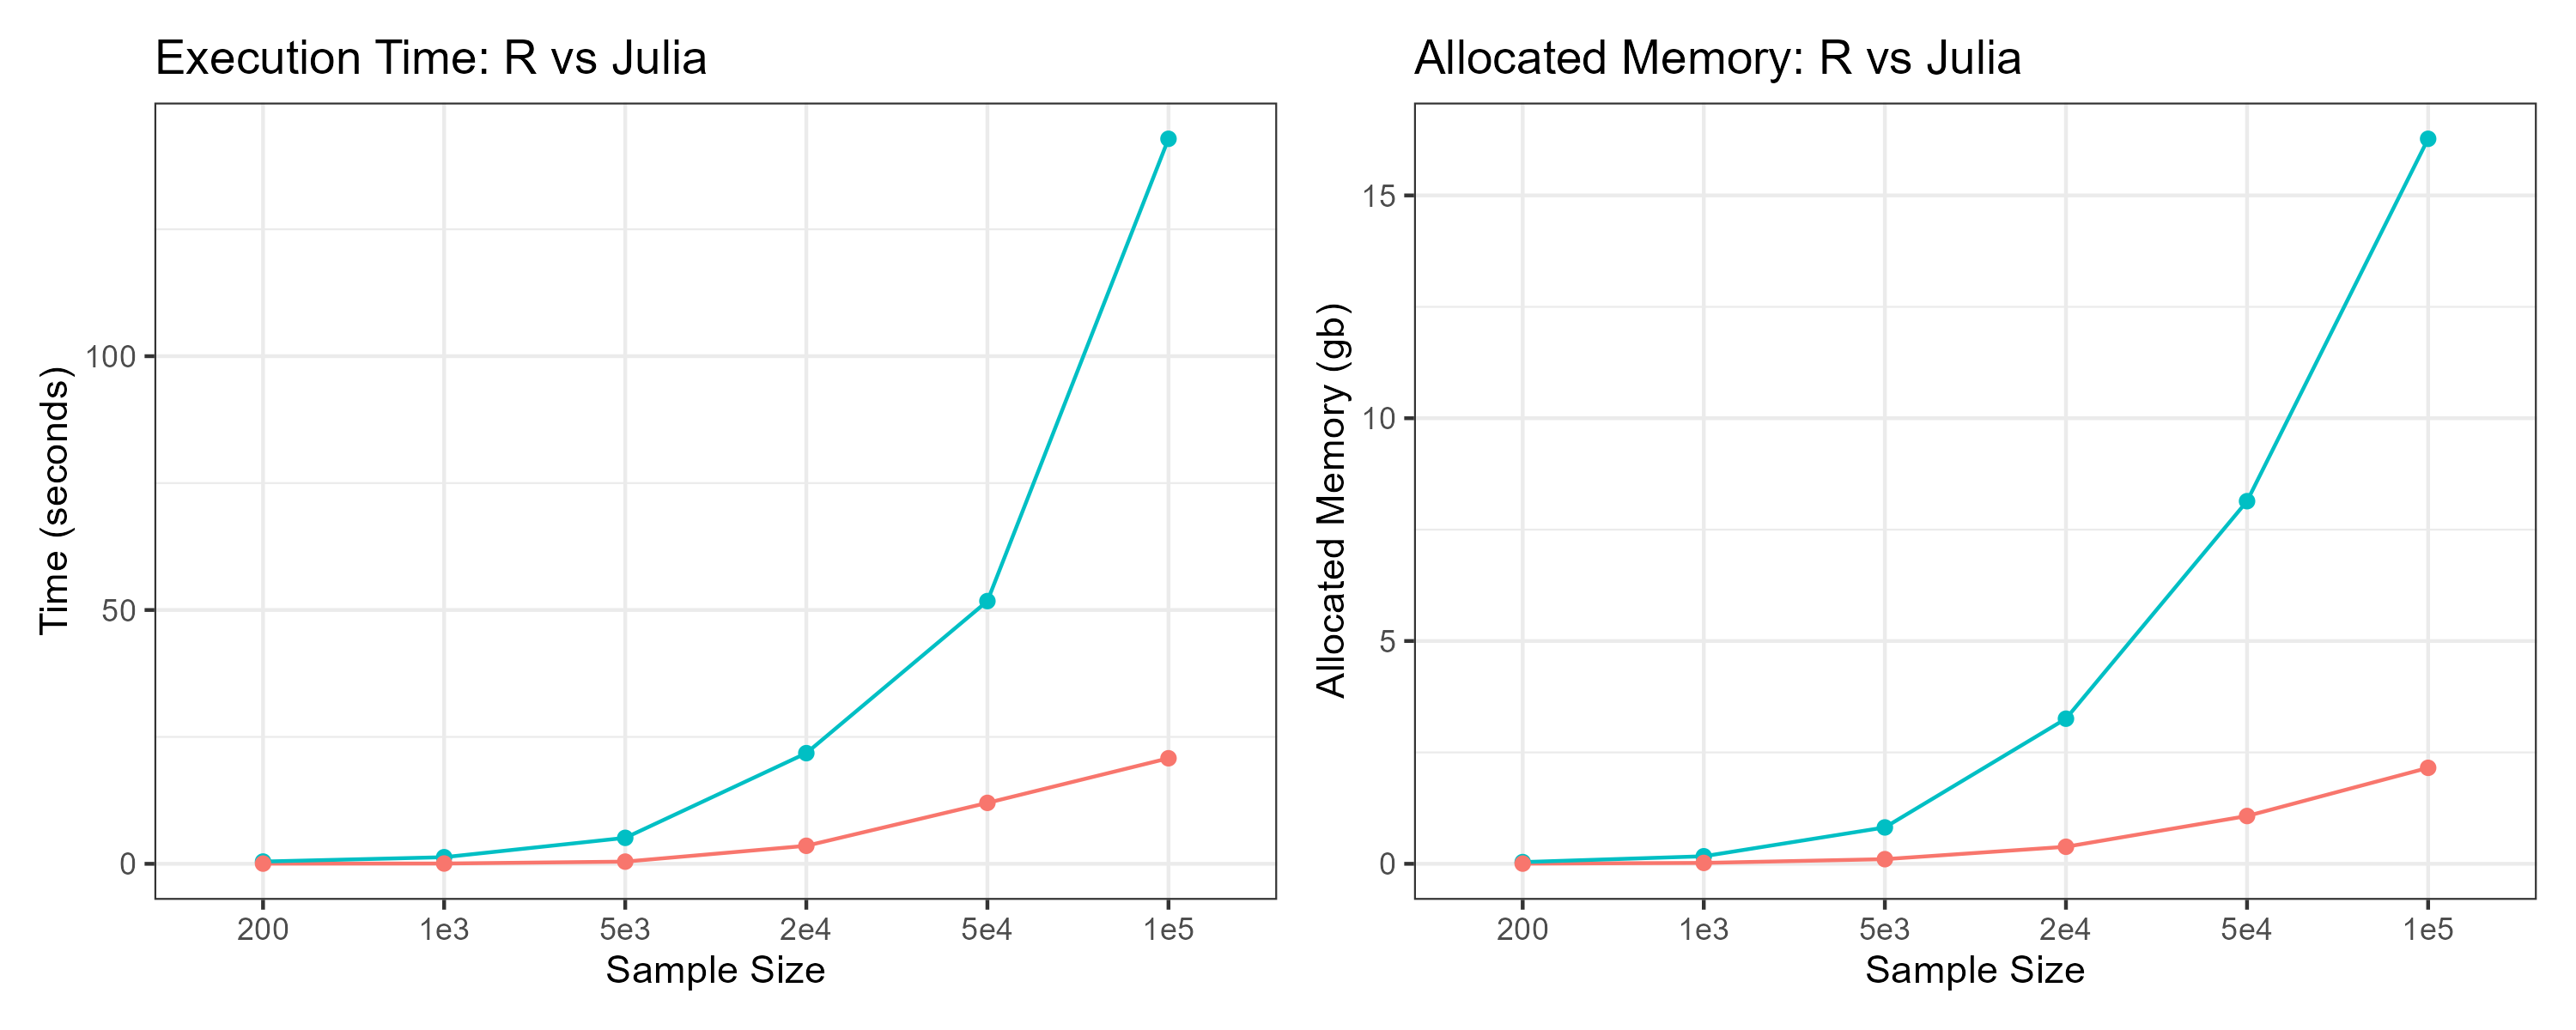
\includegraphics[width=0.95\textwidth]{plots_performance/noCI_performance.png}
\caption{Computation time and memory allocations of \textcolor{red}{\juliaTTE{}} and \textcolor{blue}{\RTTE{}} across increasing sample sizes, excluding confidence interval estimation. Results are averaged over five replications. The red line marks \textcolor{red}{\julia{}}, the blue line marks \textcolor{blue}{\Rlang{}}.}
\label{plt:speed_noCI}
\end{figure}

\begin{figure}[h]
\centering
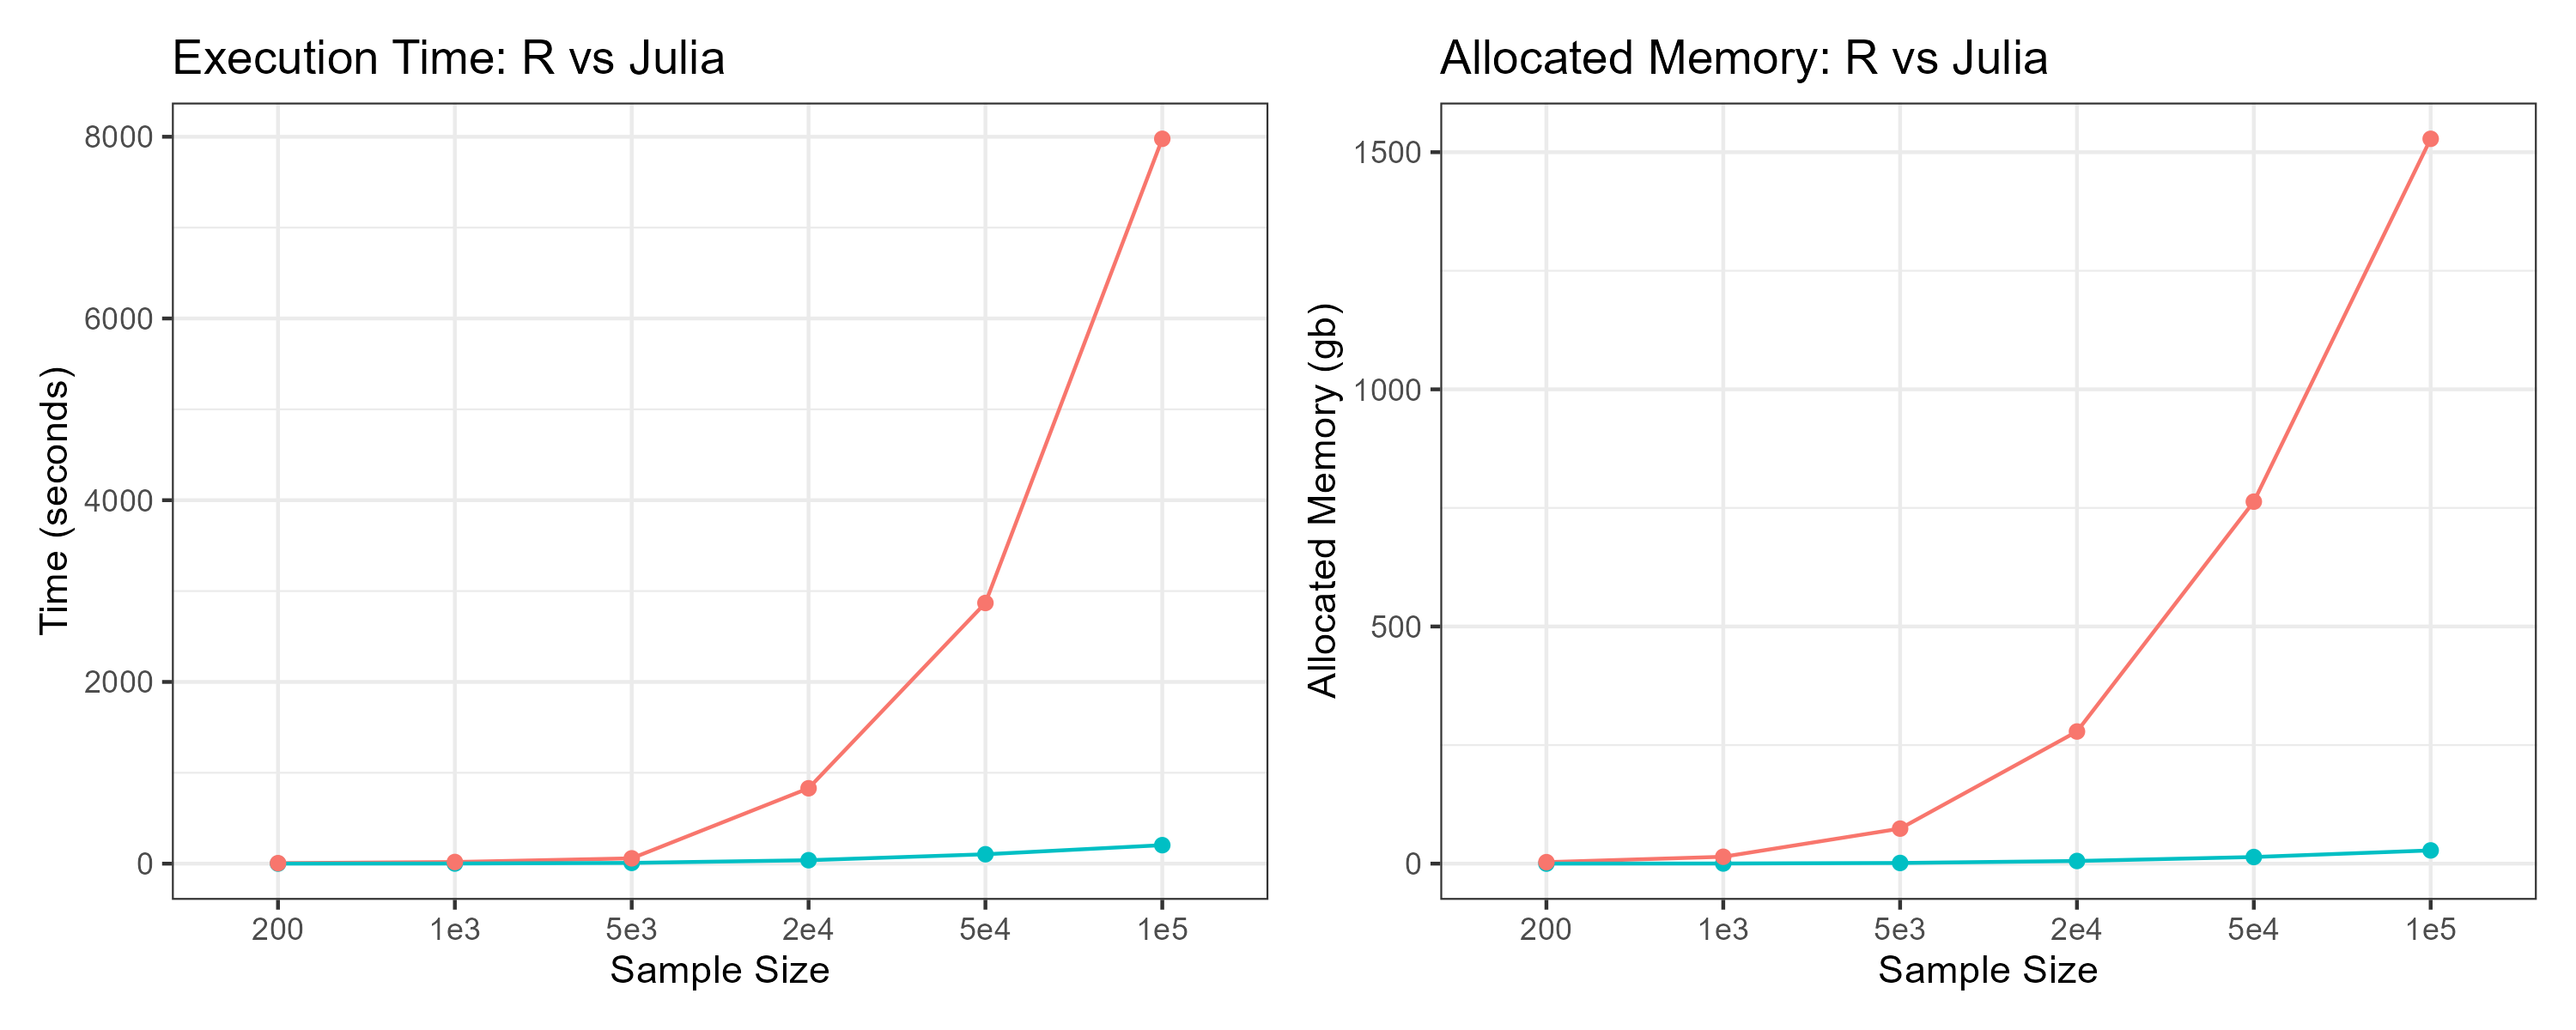
\includegraphics[width=0.95\textwidth]{plots_performance/CI_performance.png}
\caption{Computation time and memory allocations of \textcolor{red}{\juliaTTE{}} and \textcolor{blue}{\RTTE{}} across increasing sample sizes, including confidence interval estimation. Results are averaged over five replications. The red line marks \textcolor{red}{\julia{}}, the blue line marks \textcolor{blue}{\Rlang{}}.}
\label{plt:speed_CI}
\end{figure}


A limitation of the study is that \julia{} has longer pre-compilation times due to its just-in-time compiler. While this extra time is negligible in big samples, it will affect the estimation time of small samples. To adequately compare the performance of the \juliaTTE{} and the \RTTE{} package, the aim should be to closely replicate a realistic analysis scenario. This is left open for future research.

A further limitation is that only the total allocated memory was measured. While this gives a good measure of memory used and computational efficiency, to investigate possible hardware limitations, the peak memory usage (the highest amount of memory used in one process) should also be measured.

Overall, the results confirm that \julia{} provides substantial performance advantages over \Rlang{} for sequential TTE, particularly in terms of speed and memory efficiency. However, the computational cost of bootstrap resampling remains high even in \julia{}, highlighting a trade-off between estimator robustness and scalability. As concluded in Section \ref{sec:Discussion}, future research should focus on improving inference with bootstrap methods, while also enhancing computational scalability.



\pagebreak

\section{Bootstrap Distributions}\label{Apx:BS}
During the simulation outlined in Section~\ref{sec:SimulationStudy}, the bootstrap distributions were not saved. Future research on bootstrap methods for sequential TTE should save and systematically evaluate them to evaluate their performance and find indicators for possible improvements. Following, we reran one simulation scenario with all three sample sizes to show an example of the skewed distributions. While this is not a comprehensive simulation study, it indicates the bottlenecks of the currently implemented percentile and empirical bootstrap methods. 

Figures~\ref{plt:bsdist200}-\ref{plt:bsdist5000} show that all bootstrap distributions are skewed. This leads to problems in the estimation of the confidence intervals, because the empirical bootstrap method assumes approximate symmetry of the sampling distribution, which does not hold in this case, potentially resulting in biased or misleading interval bounds, as discussed in Section~\ref{sec:Discussion}.

\begin{figure}[h]
\centering
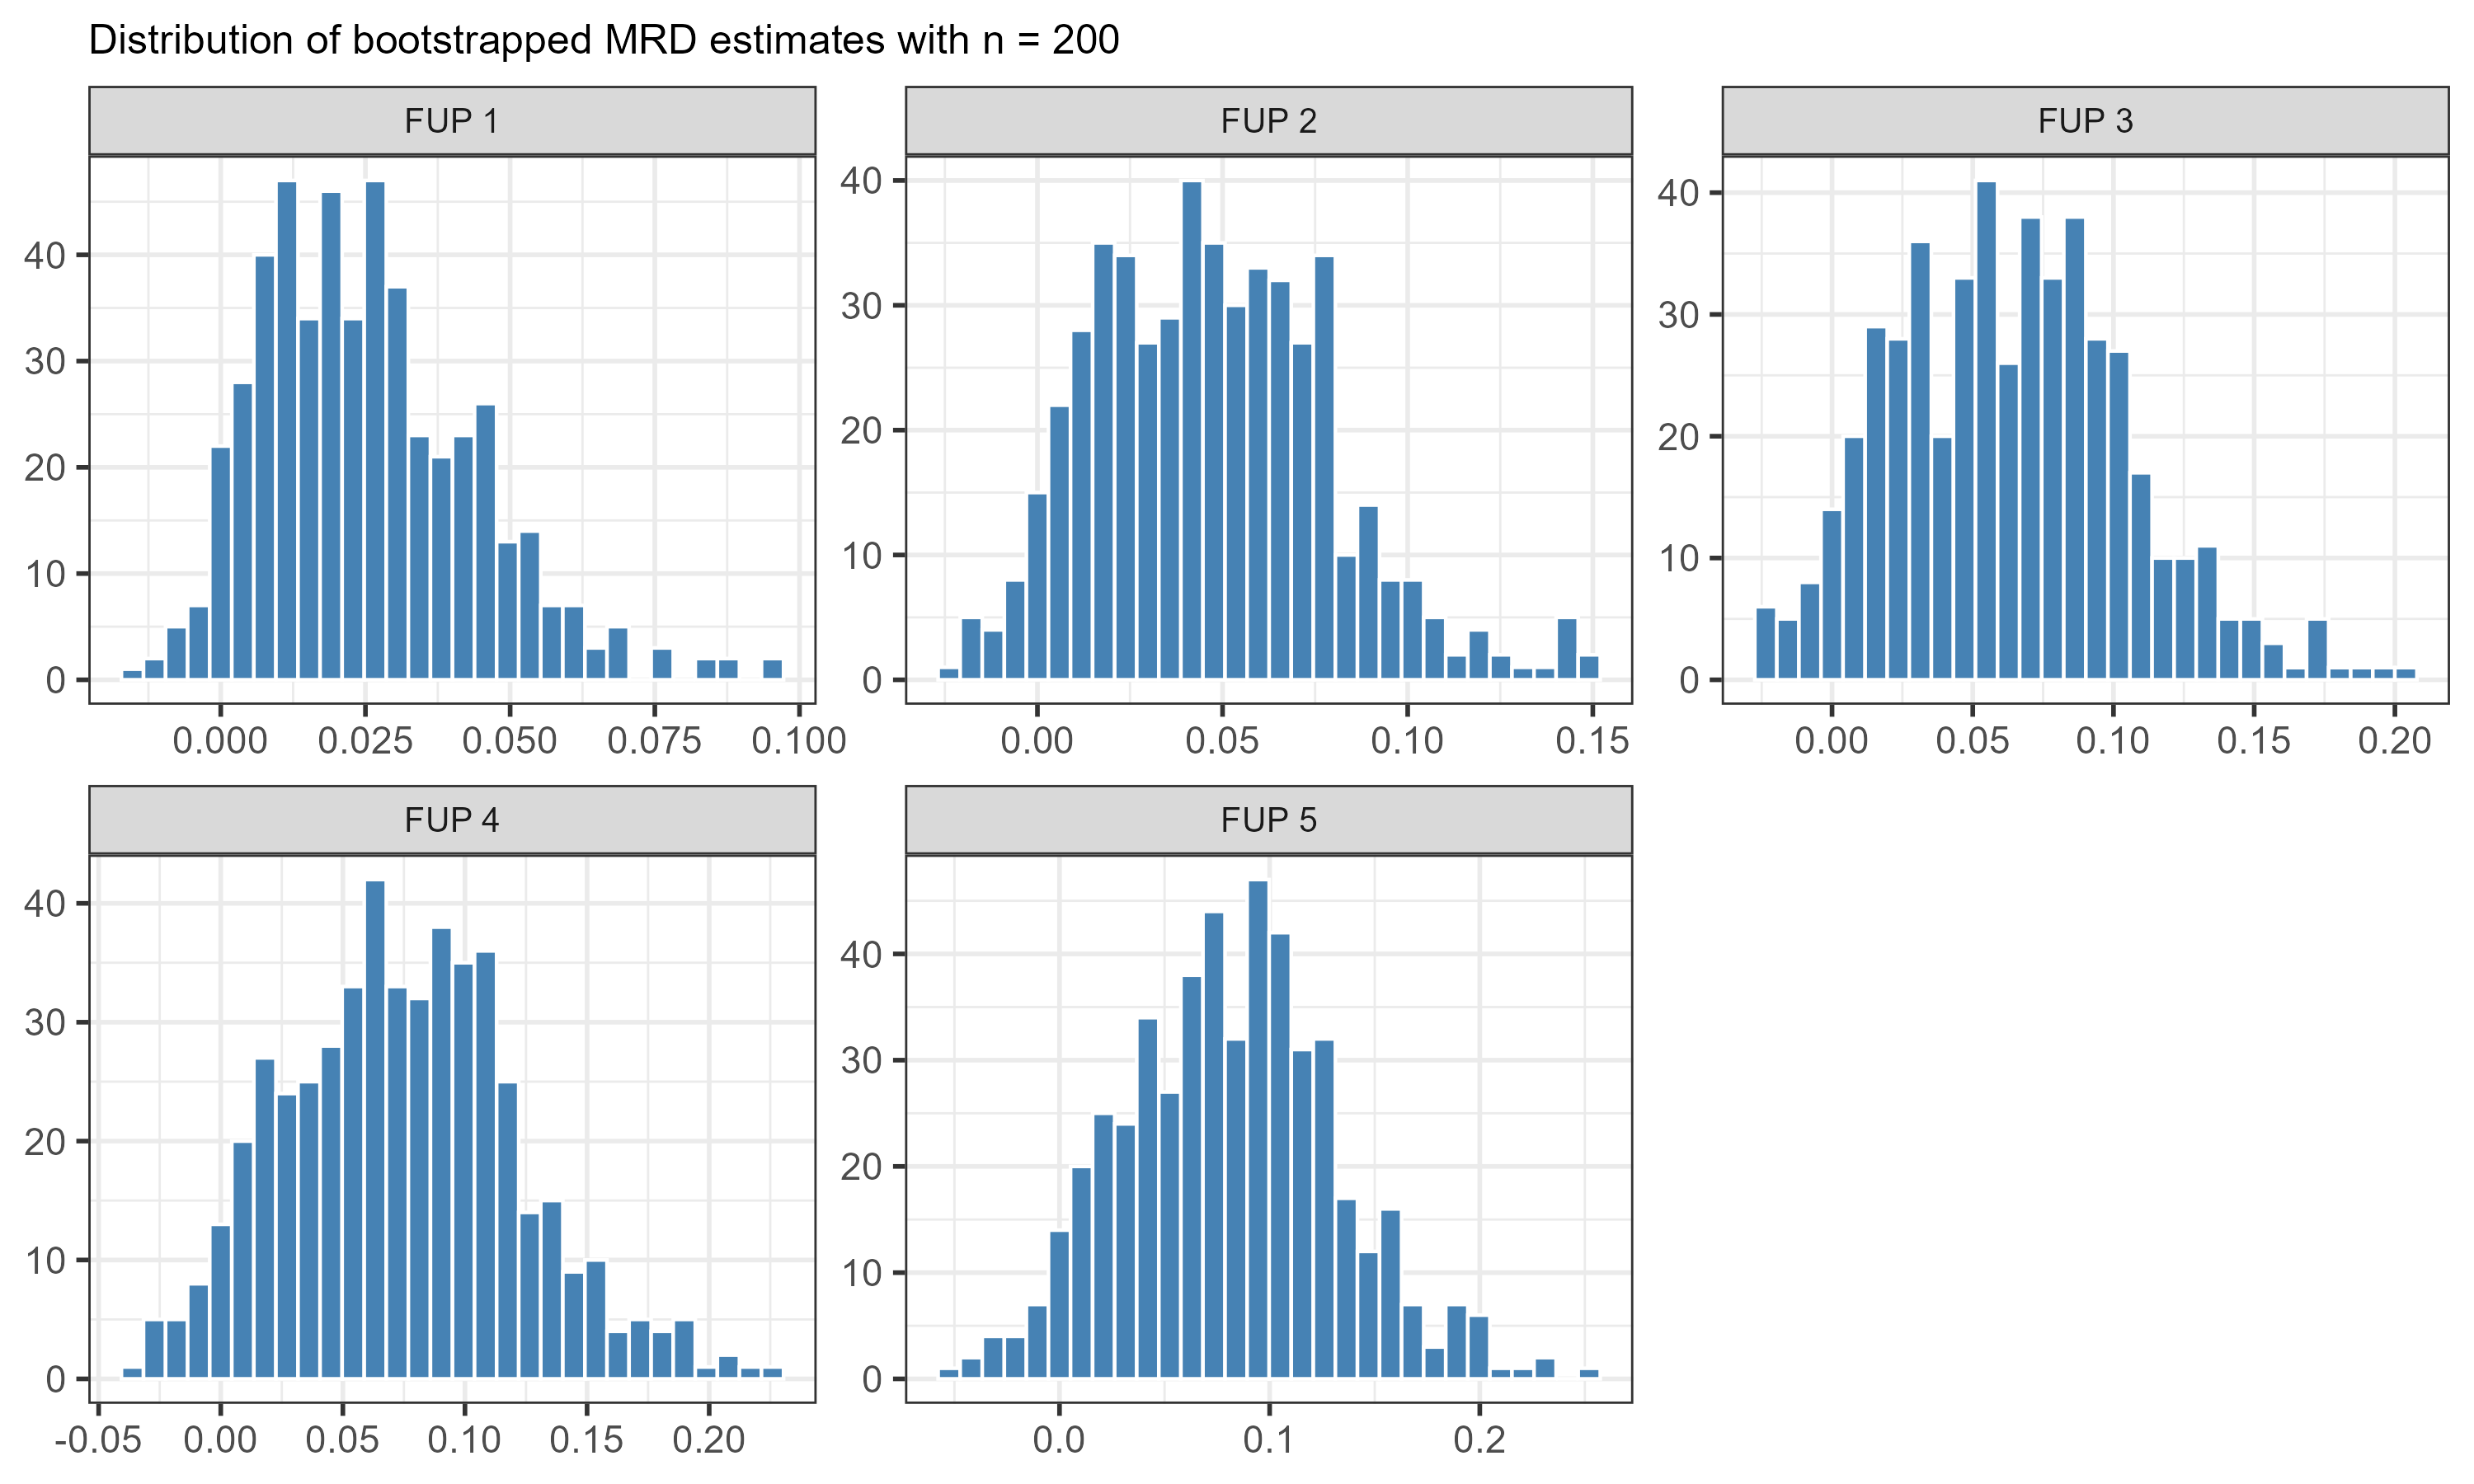
\includegraphics[width=0.95\textwidth]{plots_dist/plot_BSdist_200.png}
\caption{Distribution of bootstrapped $\widehat{\text{MRD}}$ estimates across five follow-up periods (FUP 1–5) based on $n = 200$ resamples. Each panel displays the empirical distribution of the point estimate, capturing the sampling variability of the marginal risk difference over time.}\label{plt:bsdist200}
\end{figure}

\begin{figure}[h]
\centering
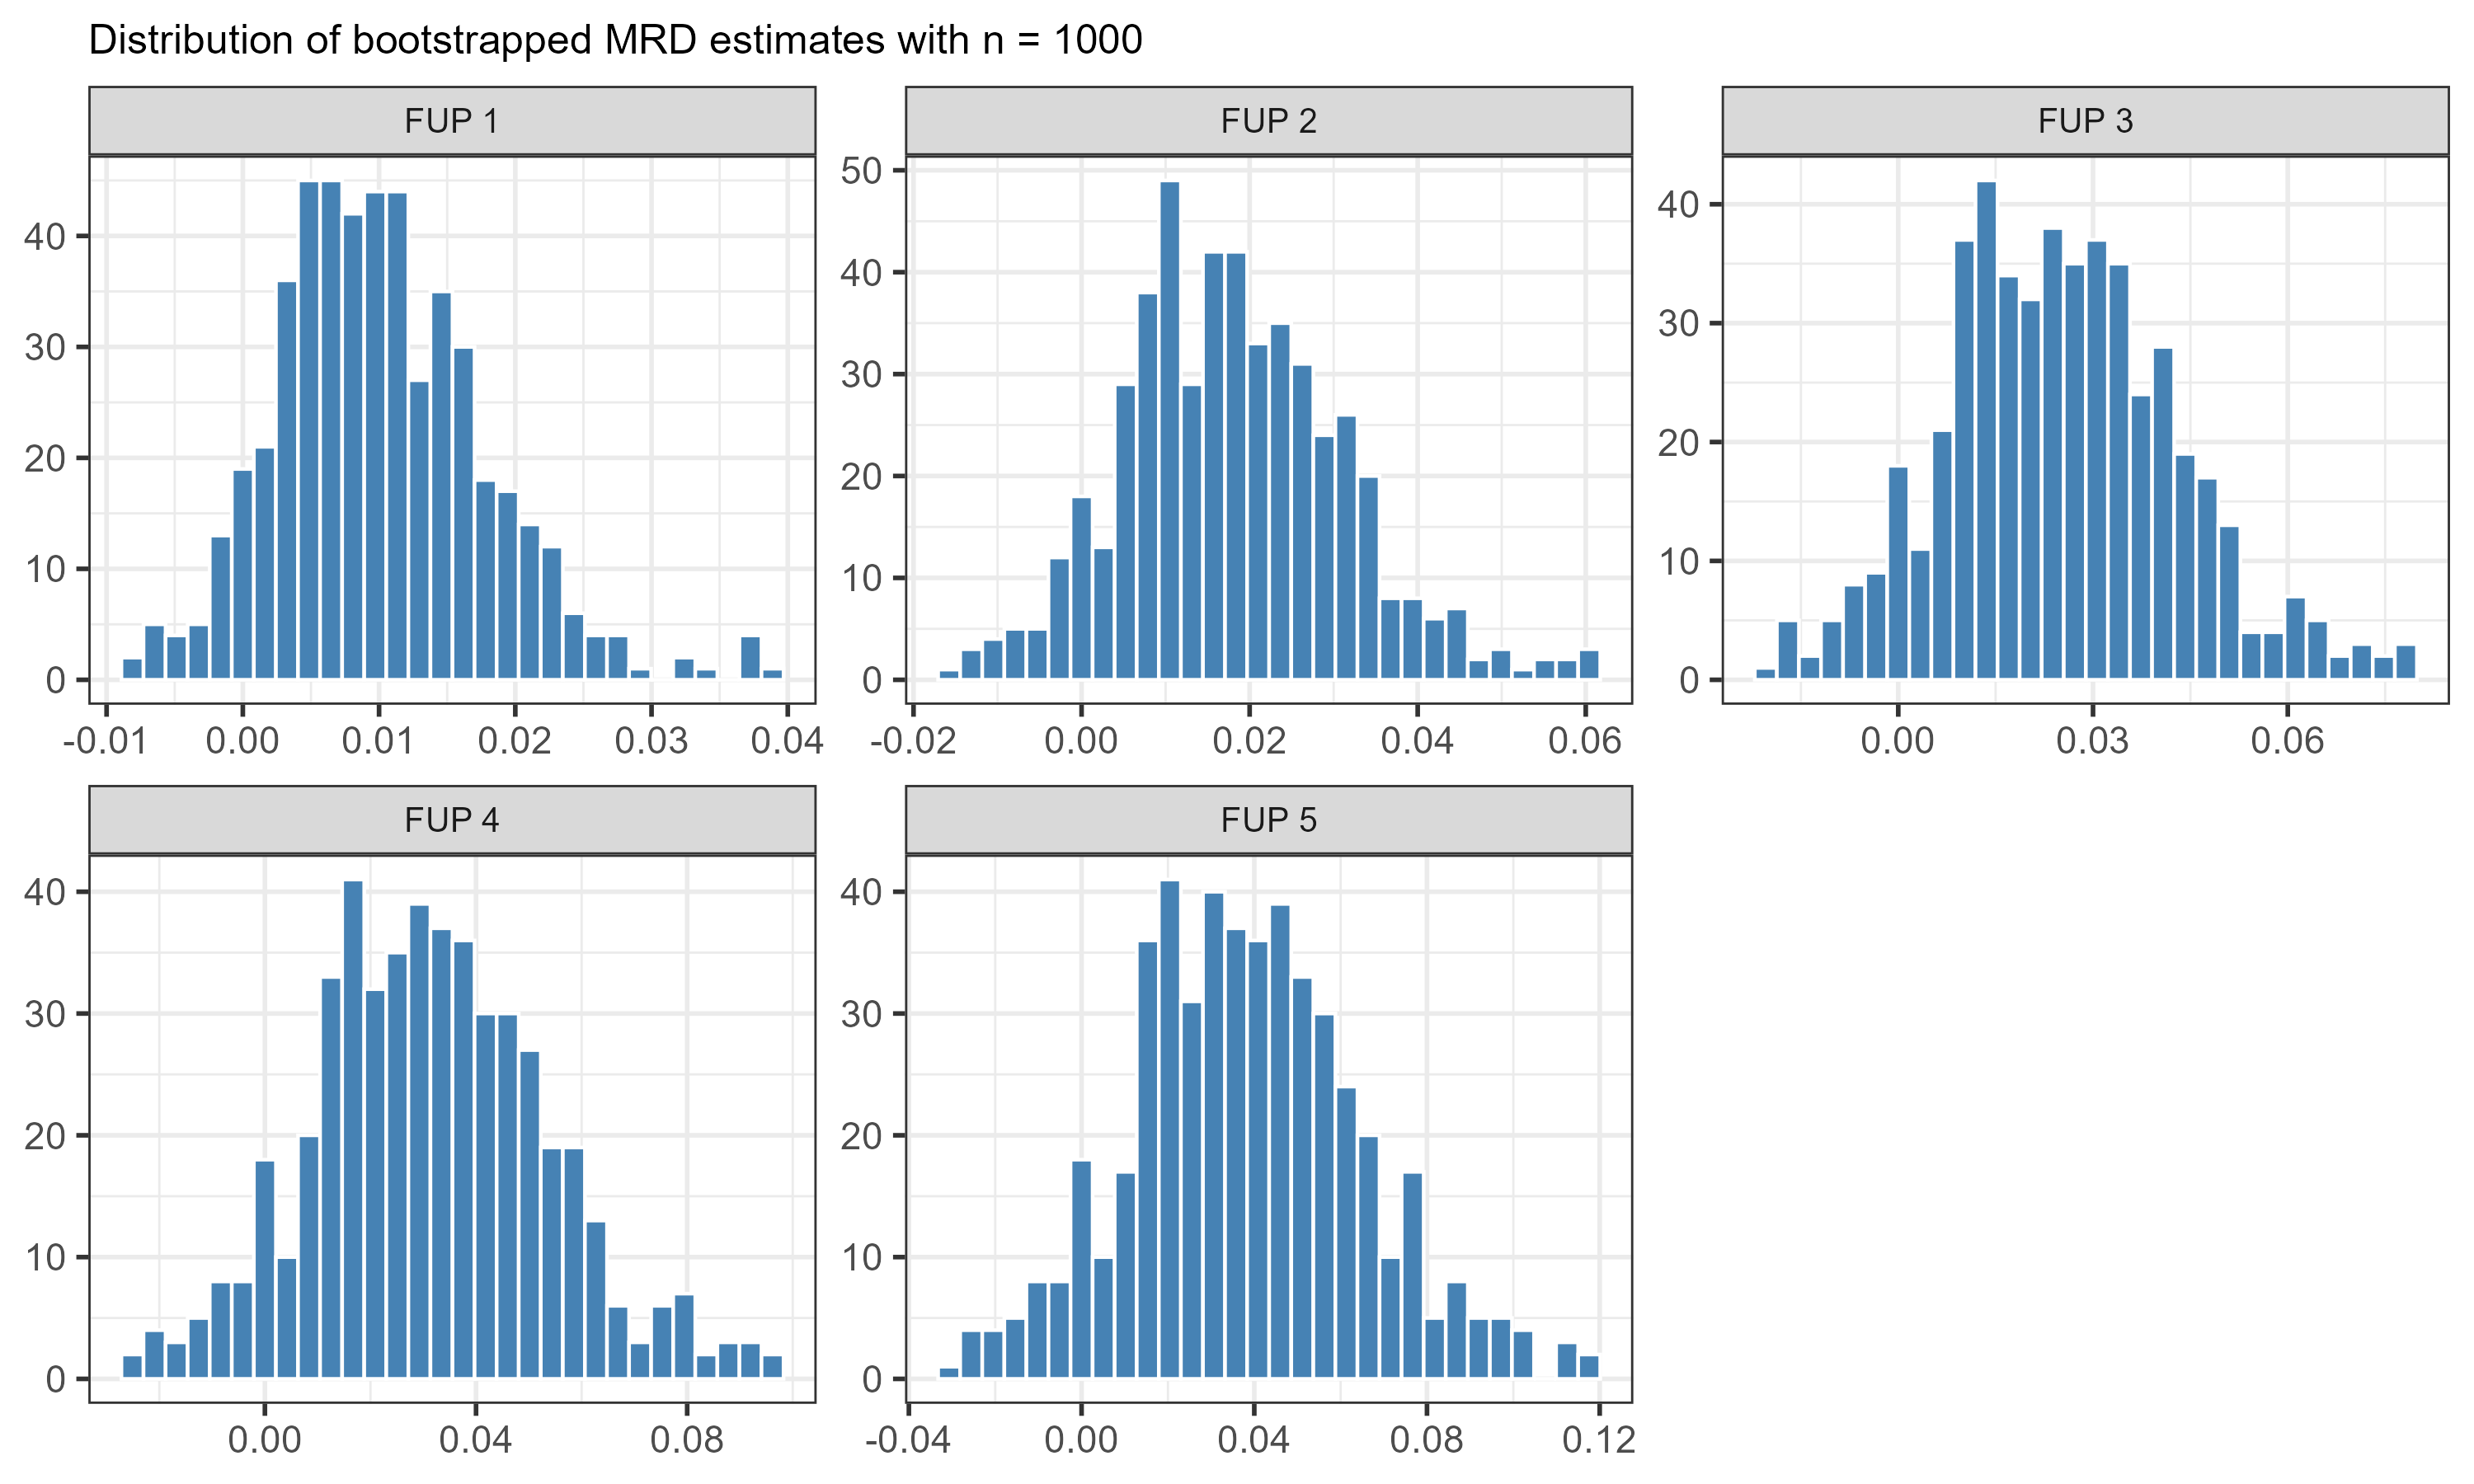
\includegraphics[width=0.95\textwidth]{plots_dist/plot_BSdist_1000.png}
\caption{Distribution of bootstrapped $\widehat{\text{MRD}}$ estimates across five follow-up periods (FUP 1–5) based on $n = 1000$ resamples. Each panel displays the empirical distribution of the point estimate, capturing the sampling variability of the marginal risk difference over time.}\label{plt:bsdist1000}
\end{figure}

\begin{figure}[h]
\centering
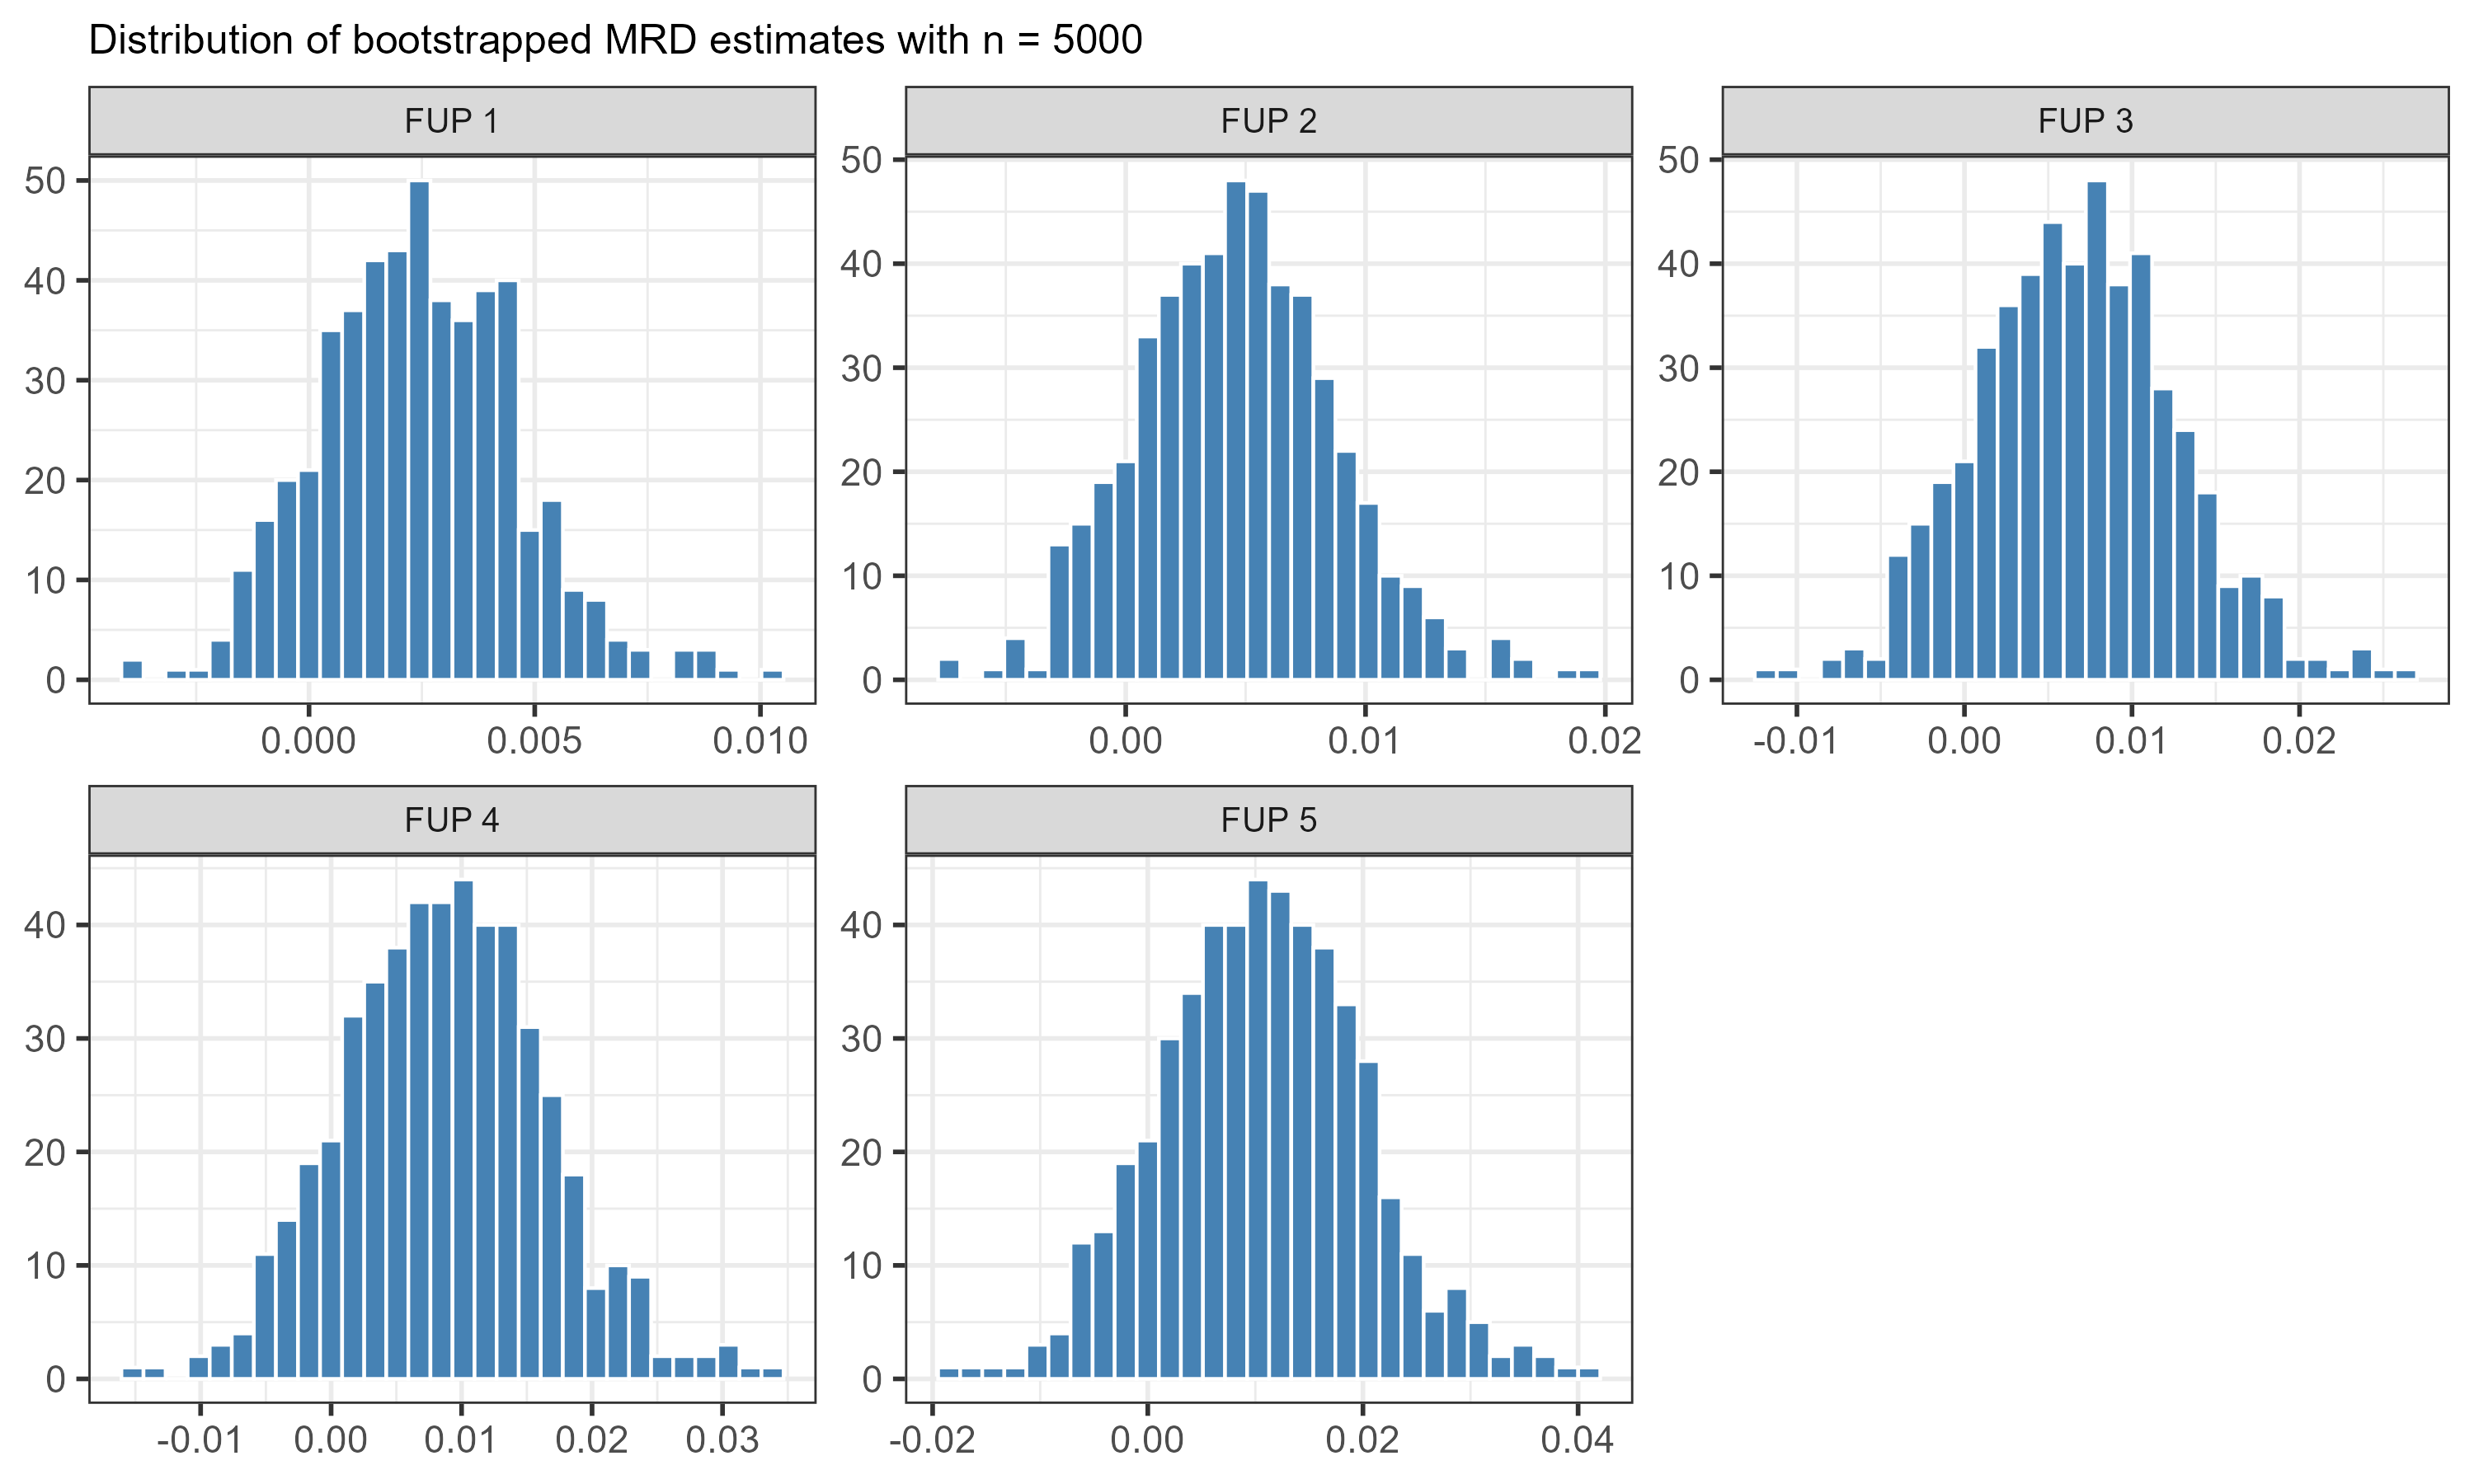
\includegraphics[width=0.95\textwidth]{plots_dist/plot_BSdist_5000.png}
\caption{Distribution of bootstrapped $\widehat{\text{MRD}}$ estimates across five follow-up periods (FUP 1–5) based on $n = 5000$ resamples. Each panel displays the empirical distribution of the point estimate, capturing the sampling variability of the marginal risk difference over time.}\label{plt:bsdist5000}
\end{figure}


%%=============================================%%
%% For submissions to Nature Portfolio Journals %%
%% please use the heading ``Extended Data''.   %%
%%=============================================%%

%%=============================================================%%
%% Sample for another appendix section			       %%
%%=============================================================%%

%% \section{Example of another appendix section}\label{secA2}%
%% Appendices may be used for helpful, supporting or essential material that would otherwise 
%% clutter, break up or be distracting to the text. Appendices can consist of sections, figures, 
%% tables and equations etc.

\end{appendices}

%%===========================================================================================%%
%% If you are submitting to one of the Nature Portfolio journals, using the eJP submission   %%
%% system, please include the references within the manuscript file itself. You may do this  %%
%% by copying the reference list from your .bbl file, paste it into the main manuscript .tex %%
%% file, and delete the associated \verb+\bibliography+ commands.                            %%
%%===========================================================================================%%



\end{document}
